%%____________________________________________________________________________||
\section{Results (original plots)}
\label{app:results-orig}

The section includes the figures that summarised the fit results in
the previous version of this Analysis Note (v4) which have now been
superseded by Figs.~\ref{fig:no-fit}--\ref{fig:full-fit} in
Sec.~\ref{sec:results}. This section will be removed in the next
iteration of the AN.

\subsection{Monojet topology}
\label{app:results-orig-mono}

Figures~\ref{fig:mr_mono_pre} and \ref{fig:mr_mono_post} summarise the
event yields observed in data and SM expectations with their
associated uncertainties as a function of \nb and \scalht (equivalent
to \mht) for the monojet category ($\njet = 1$) for the masked and
full fits, respectively. The lower panels show the data-to-background
ratios for the masked and full fits.  Figure~\ref{fig:mr_mono_pulls}
shows background expectations for the masked fit in the upper panel,
as shown in Fig.~\ref{fig:mr_mono_pre}, and the pulls (\ie the
difference between data and the background estimates relative to their
uncertainties) for both the masked and full fits in the lower panel.

\clearpage
\begin{figure}[h!]
  \centering
  \caption{Upper panel. Event yields observed in data (solid circles)
    and SM expectations with their associated uncertainties (black
    histogram with shaded band) as a function of \nb and \scalht,
    integrated over \mht, and for the monojet category ($\njet = 1$)
    in the signal region. Lower panel. Data-to-background ratios. The
    background estimates and ratios are from the masked fit. }
  \label{fig:mr_mono_pre}
  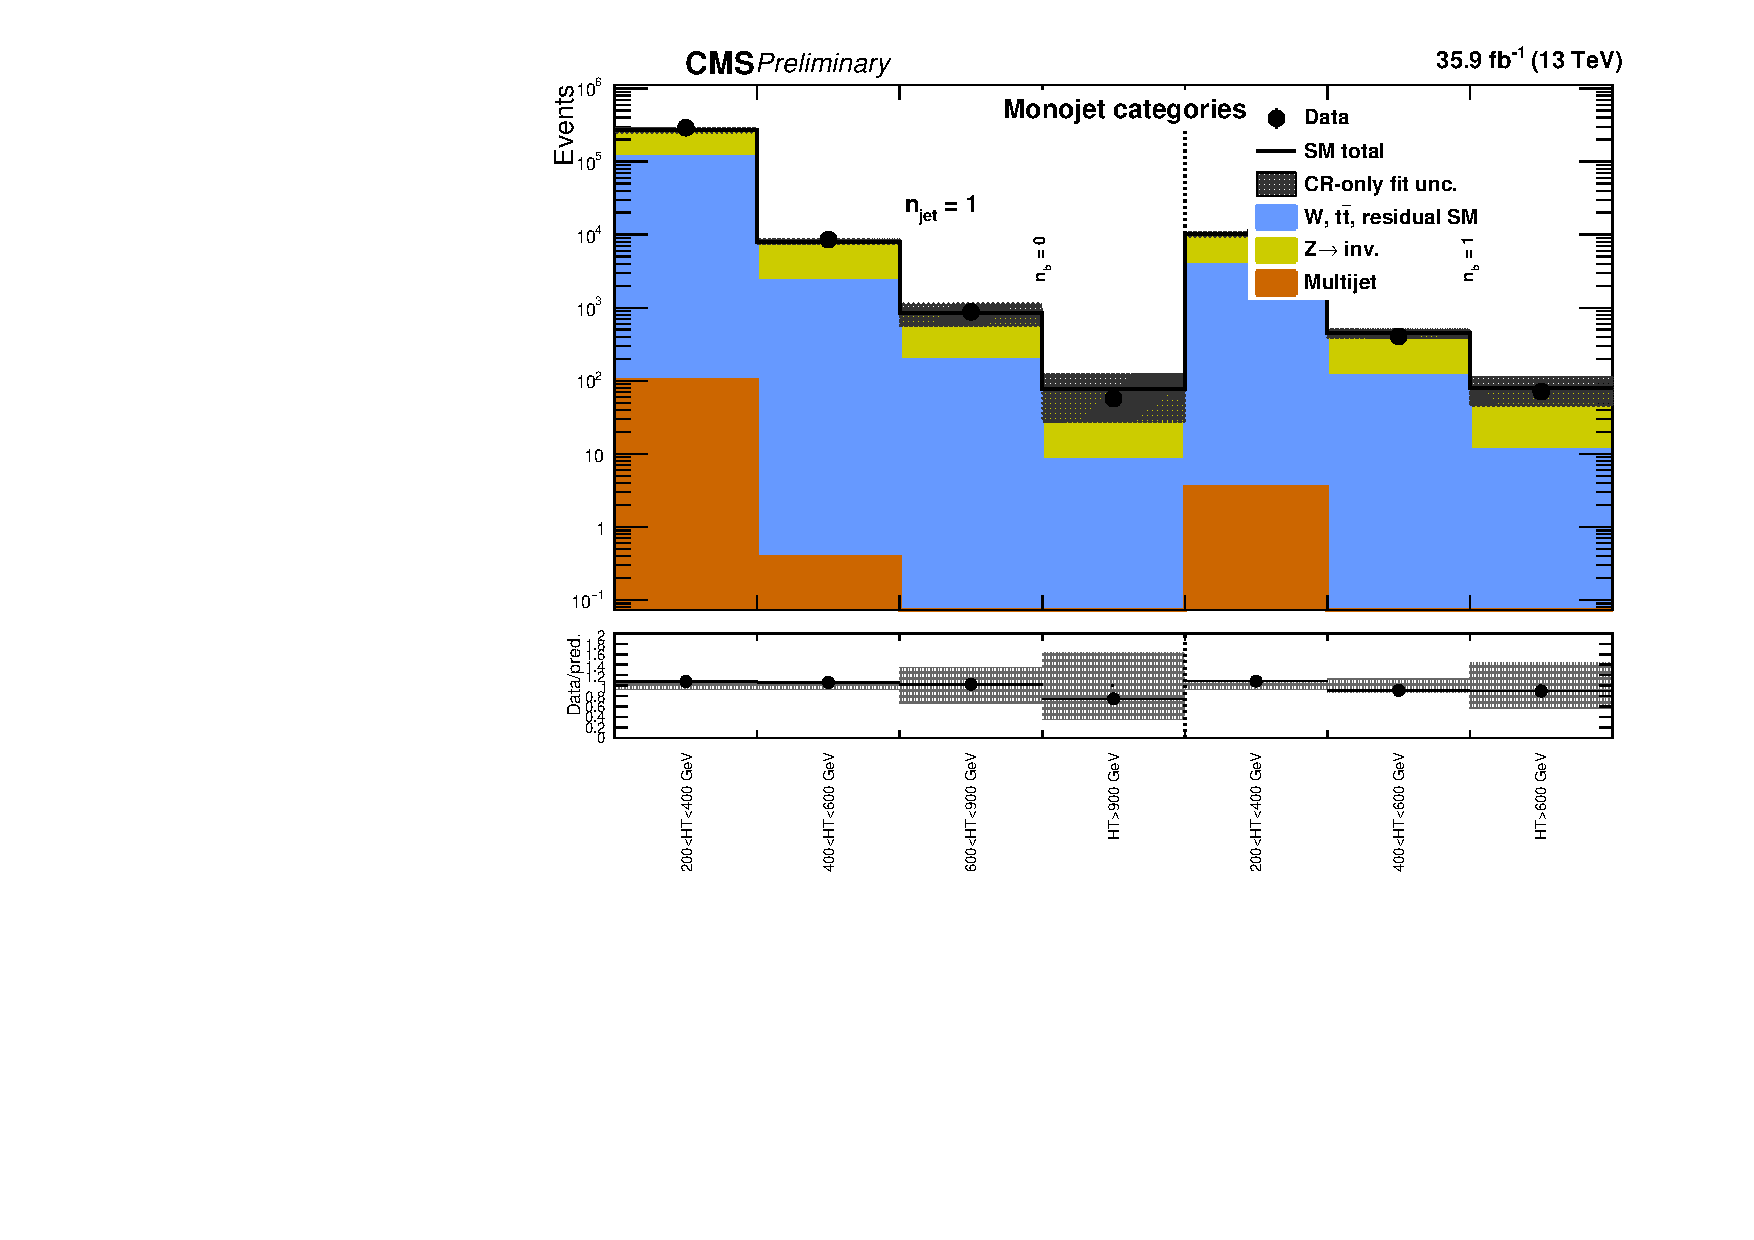
\includegraphics[width=1.\linewidth]{figures/results/36invfb_preapproval/mono/summaryPlot_Monojet_prefit}
\end{figure}

\clearpage
\begin{figure}[h!]
  \centering
  \caption{Upper panel. Event yields observed in data (solid circles)
    and SM expectations with their associated uncertainties (black
    histogram with shaded band) as a function of \nb and \scalht,
    integrated over \mht, and for the monojet category ($\njet = 1$)
    in the signal region. Lower panel. Data-to-background ratios. The
    background estimates and ratios are obtained with the full fit. }
  \label{fig:mr_mono_post}
  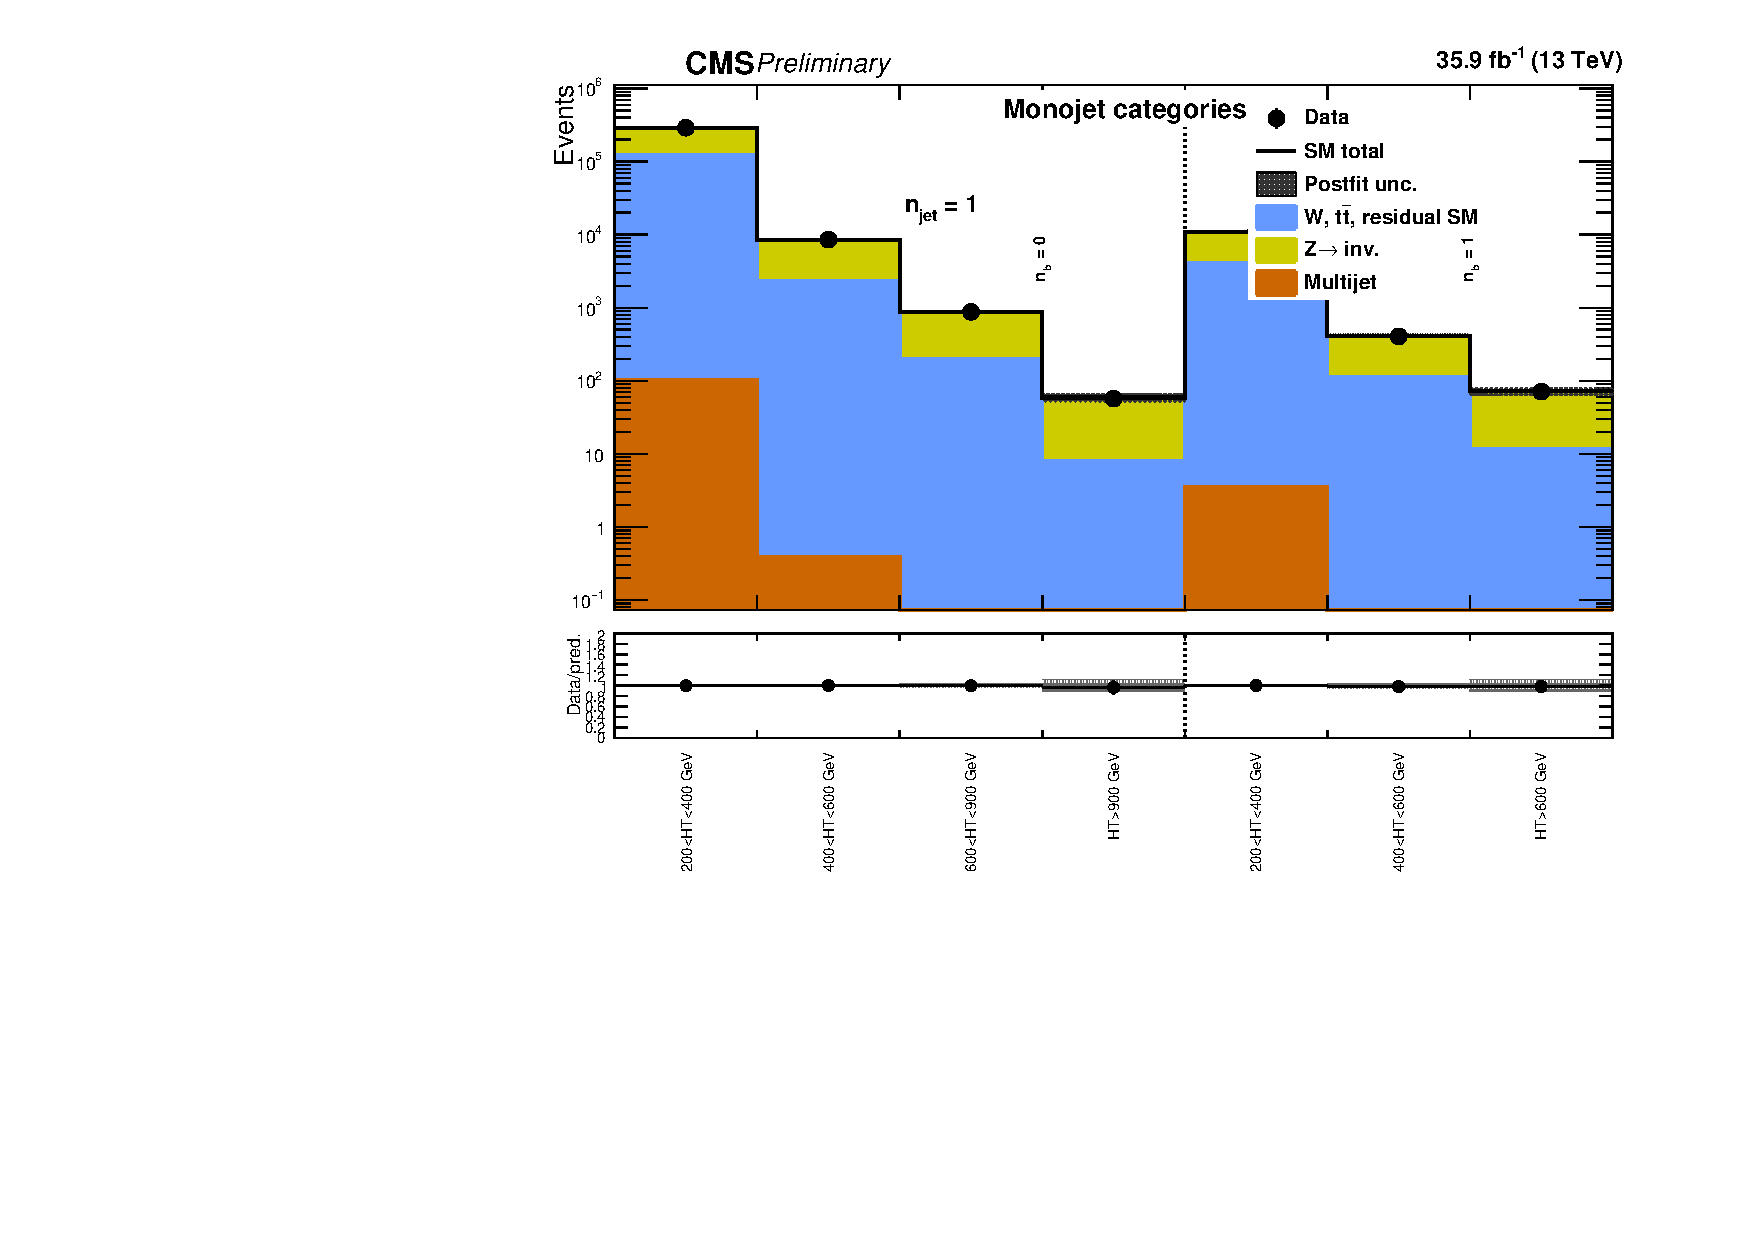
\includegraphics[width=1.\linewidth]{figures/results/36invfb_preapproval/mono/summaryPlot_Monojet_fit_b}
\end{figure}

\clearpage
\begin{figure}[h!]
  \centering
  \caption{Upper panel. Event yields observed in data (solid circles)
    and SM expectations with their associated uncertainties (black
    histogram with shaded band) as a function of \nb and \scalht,
    integrated over \mht, and for the monojet category ($\njet = 1$)
    in the signal region. Lower panel. The pulls, which are obtained
    from both the masked (red markers) and full (blue markers) fits. }
  \label{fig:mr_mono_pulls}
  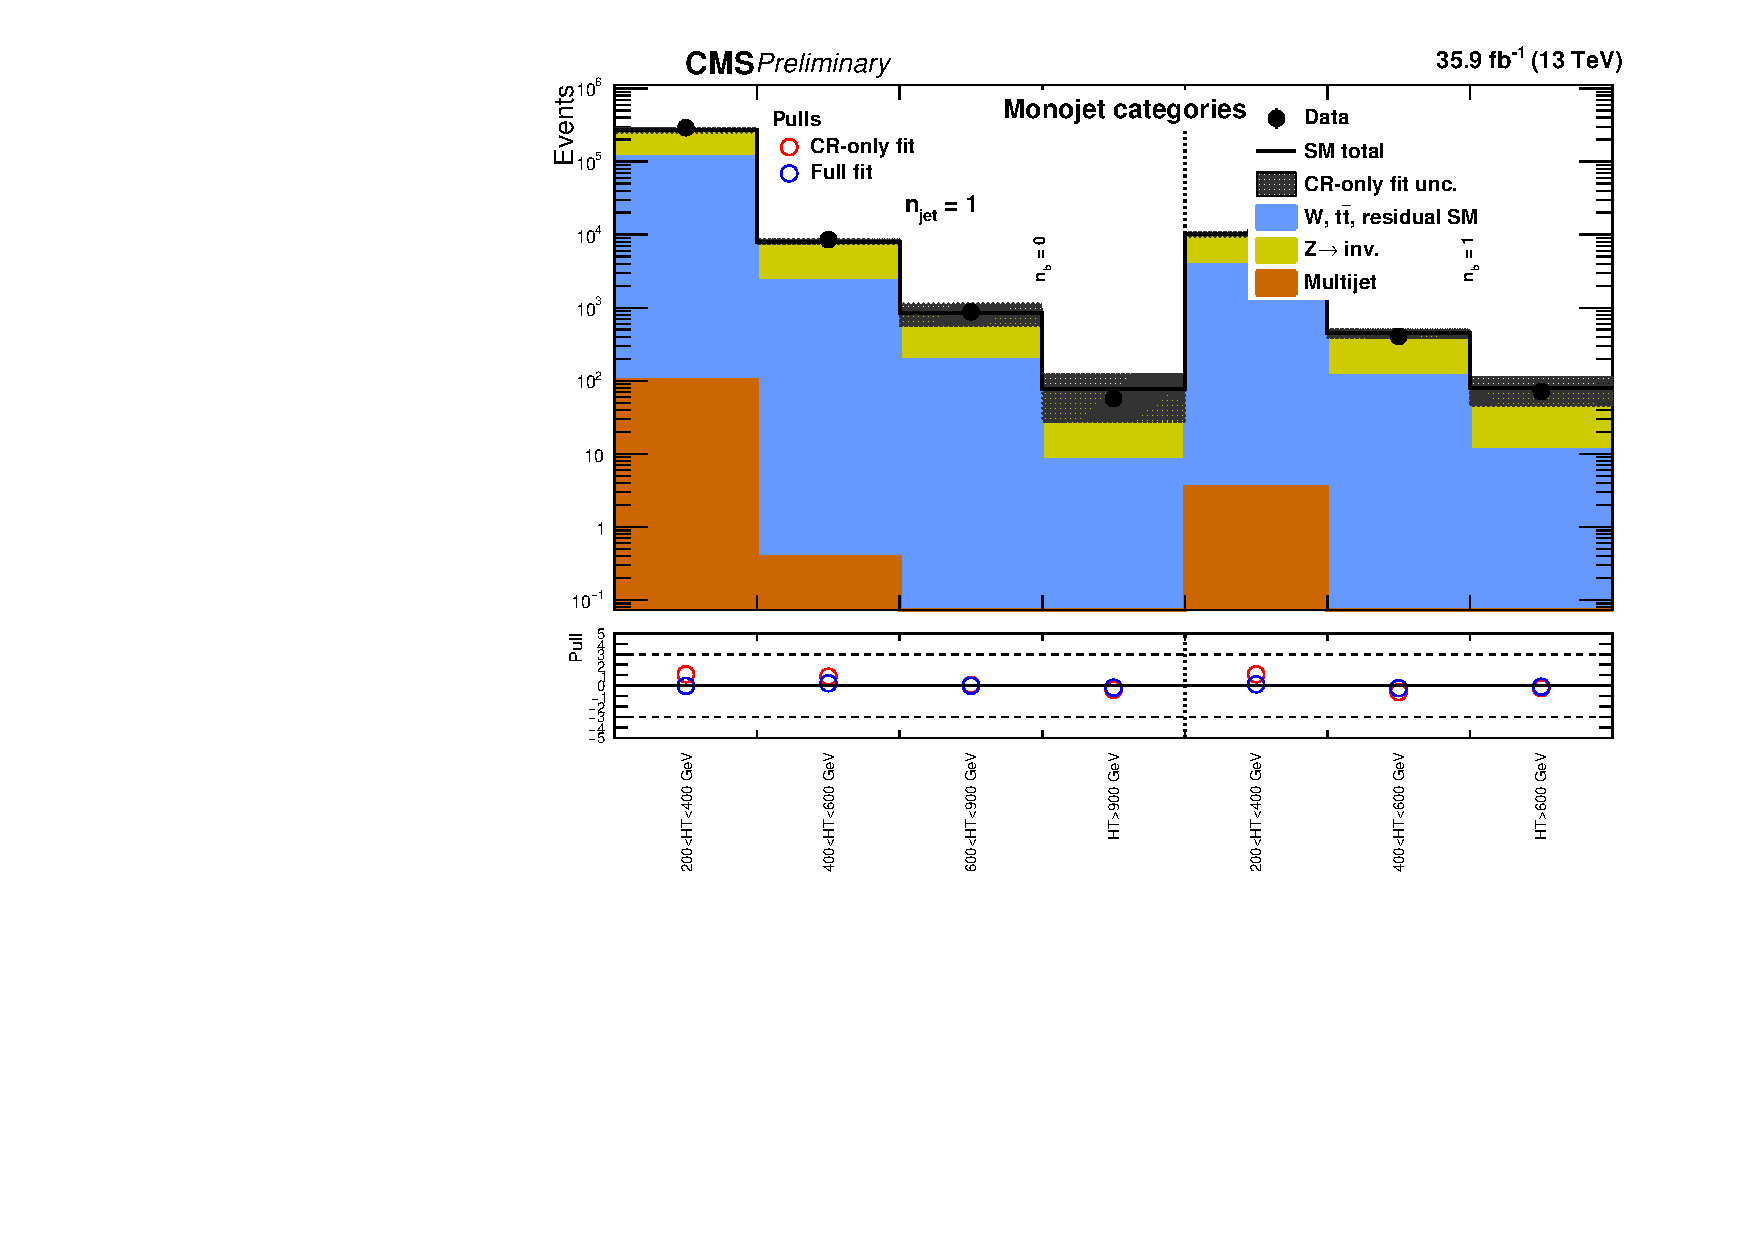
\includegraphics[width=1.\linewidth]{figures/results/36invfb_preapproval/mono/summaryPlot_Monojet_prefit_overlay_fit_b}
\end{figure}

\clearpage
\subsection{Asymmetric topology}
\label{app:results-orig-asym}

Figures~\ref{fig:mr_asym_pre} and \ref{fig:mr_asym_post} summarise the
event yields observed in data and SM expectations with their
associated uncertainties as a function of \scalht and \nb, {\it
  integated over \mht}, for the monojet category ($\njet = 1$) for the
masked and full fits, respectively. The lower panels show the
data-to-background ratios for the masked and full fits.
Figure~\ref{fig:mr_asym_pulls} shows background expectations for the
masked fit in the upper panel, as shown in Fig.~\ref{fig:mr_asym_pre},
and the pulls (\ie the difference between data and the background
estimates relative to their uncertainties) for both the masked and
full fits in the lower panel.

Figures~\ref{fig:mhtdim_ge2a_eq0b}--\ref{fig:mhtdim_ge2a_eq2b}
summarise the observed event yields and CR-fit SM expectations with
their associated uncertainties as a function of \HTmiss for based on a
sample of events that satisfy $\njet \geq 2 \; \textrm{(asymmetric)}$
and requirements on \nb and \scalht.

\clearpage
\begin{figure}[h!]
  \centering
  \caption{Upper panel. Event yields observed in data (solid circles)
    and SM expectations with their associated uncertainties (black
    histogram with shaded band) as a function of \nb and \scalht,
    integrated over \mht, and for the asymmetric \njet category
    in the signal region. Lower panel. Data-to-background ratios. The
    background estimates and ratios are from the masked fit. }
  \label{fig:mr_asym_pre}
  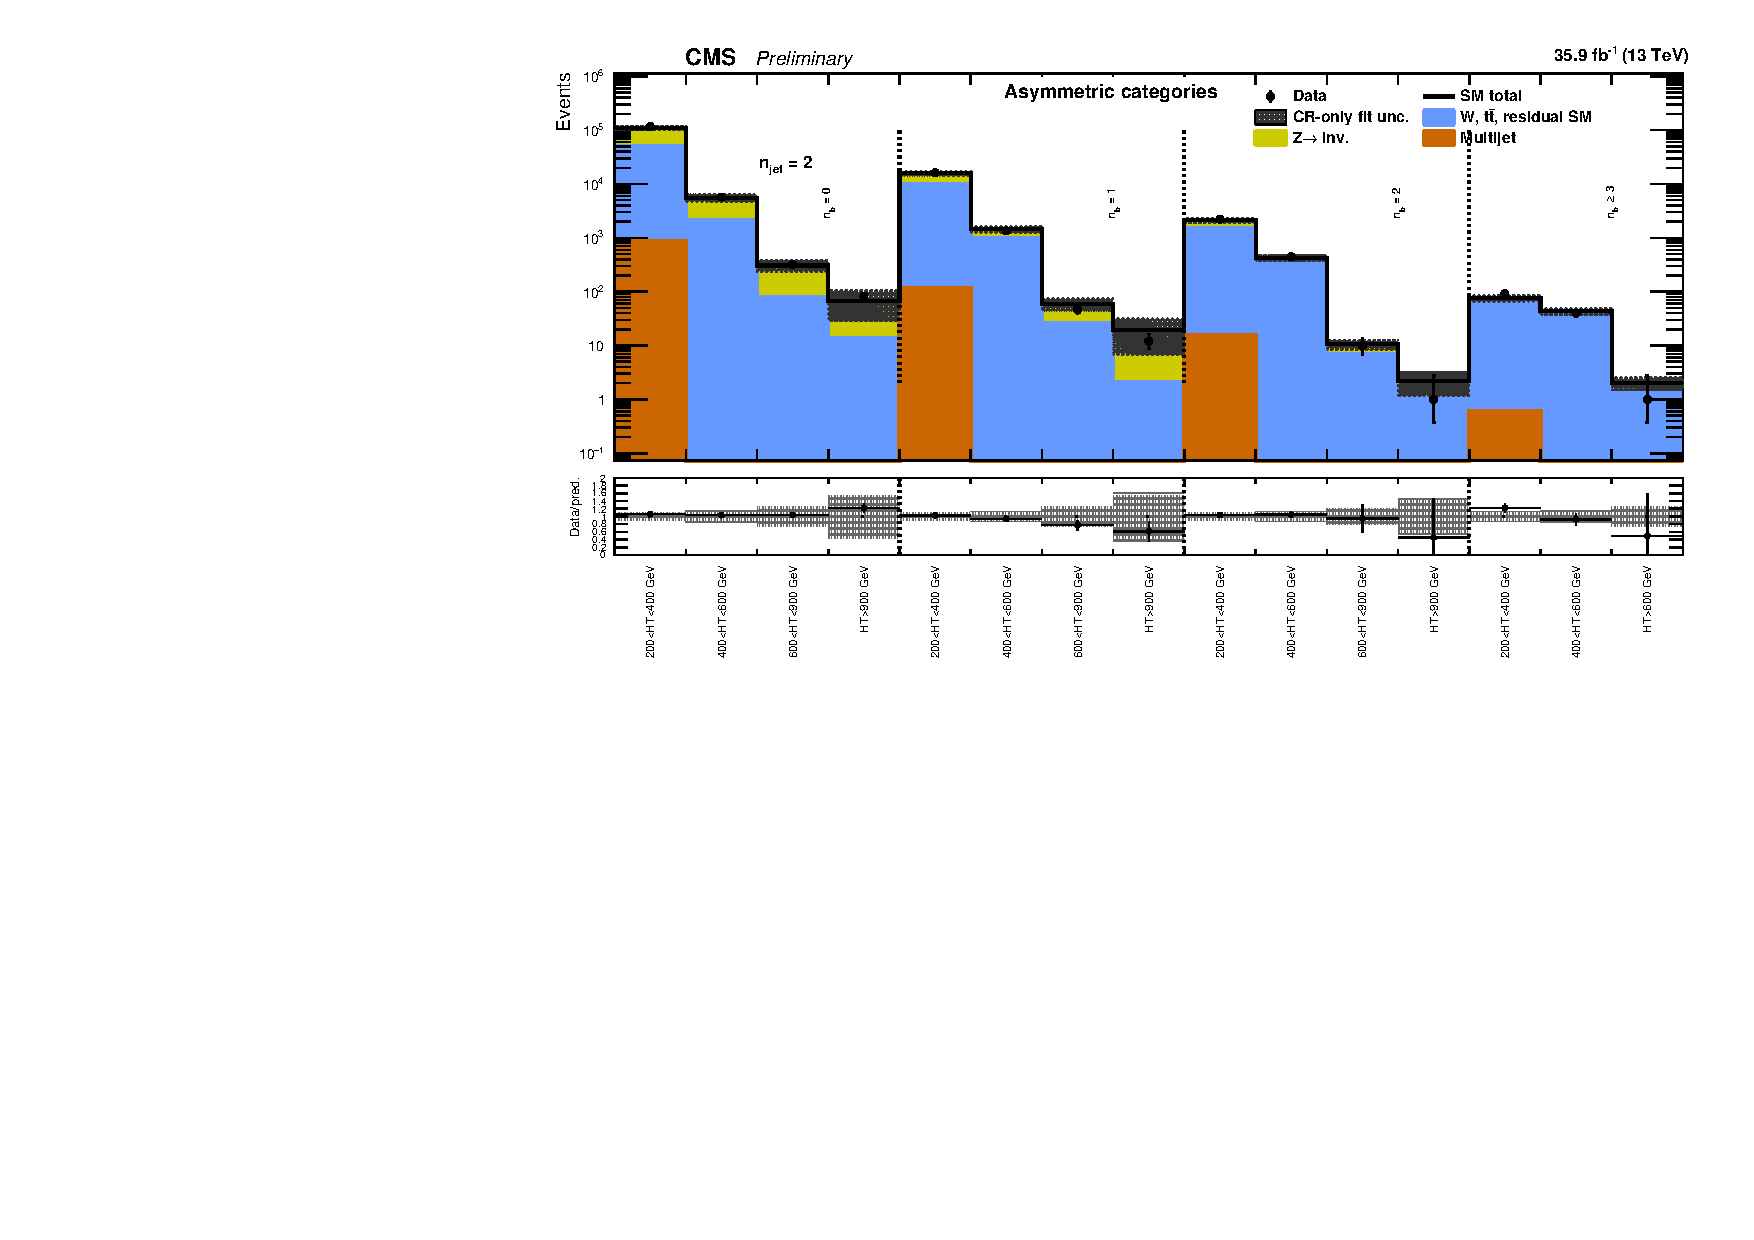
\includegraphics[width=1.\linewidth]{figures/results/36invfb_preapproval/asym/summaryPlot_Asymmetric_prefit}
\end{figure}

\clearpage
\begin{figure}[h!]
  \centering
  \caption{Upper panel. Event yields observed in data (solid circles)
    and SM expectations with their associated uncertainties (black
    histogram with shaded band) as a function of \nb and \scalht,
    integrated over \mht, and for the asymmetric \njet category
    in the signal region. Lower panel. Data-to-background ratios. The
    background estimates and ratios are obtained with the full fit. }
  \label{fig:mr_asym_post}
  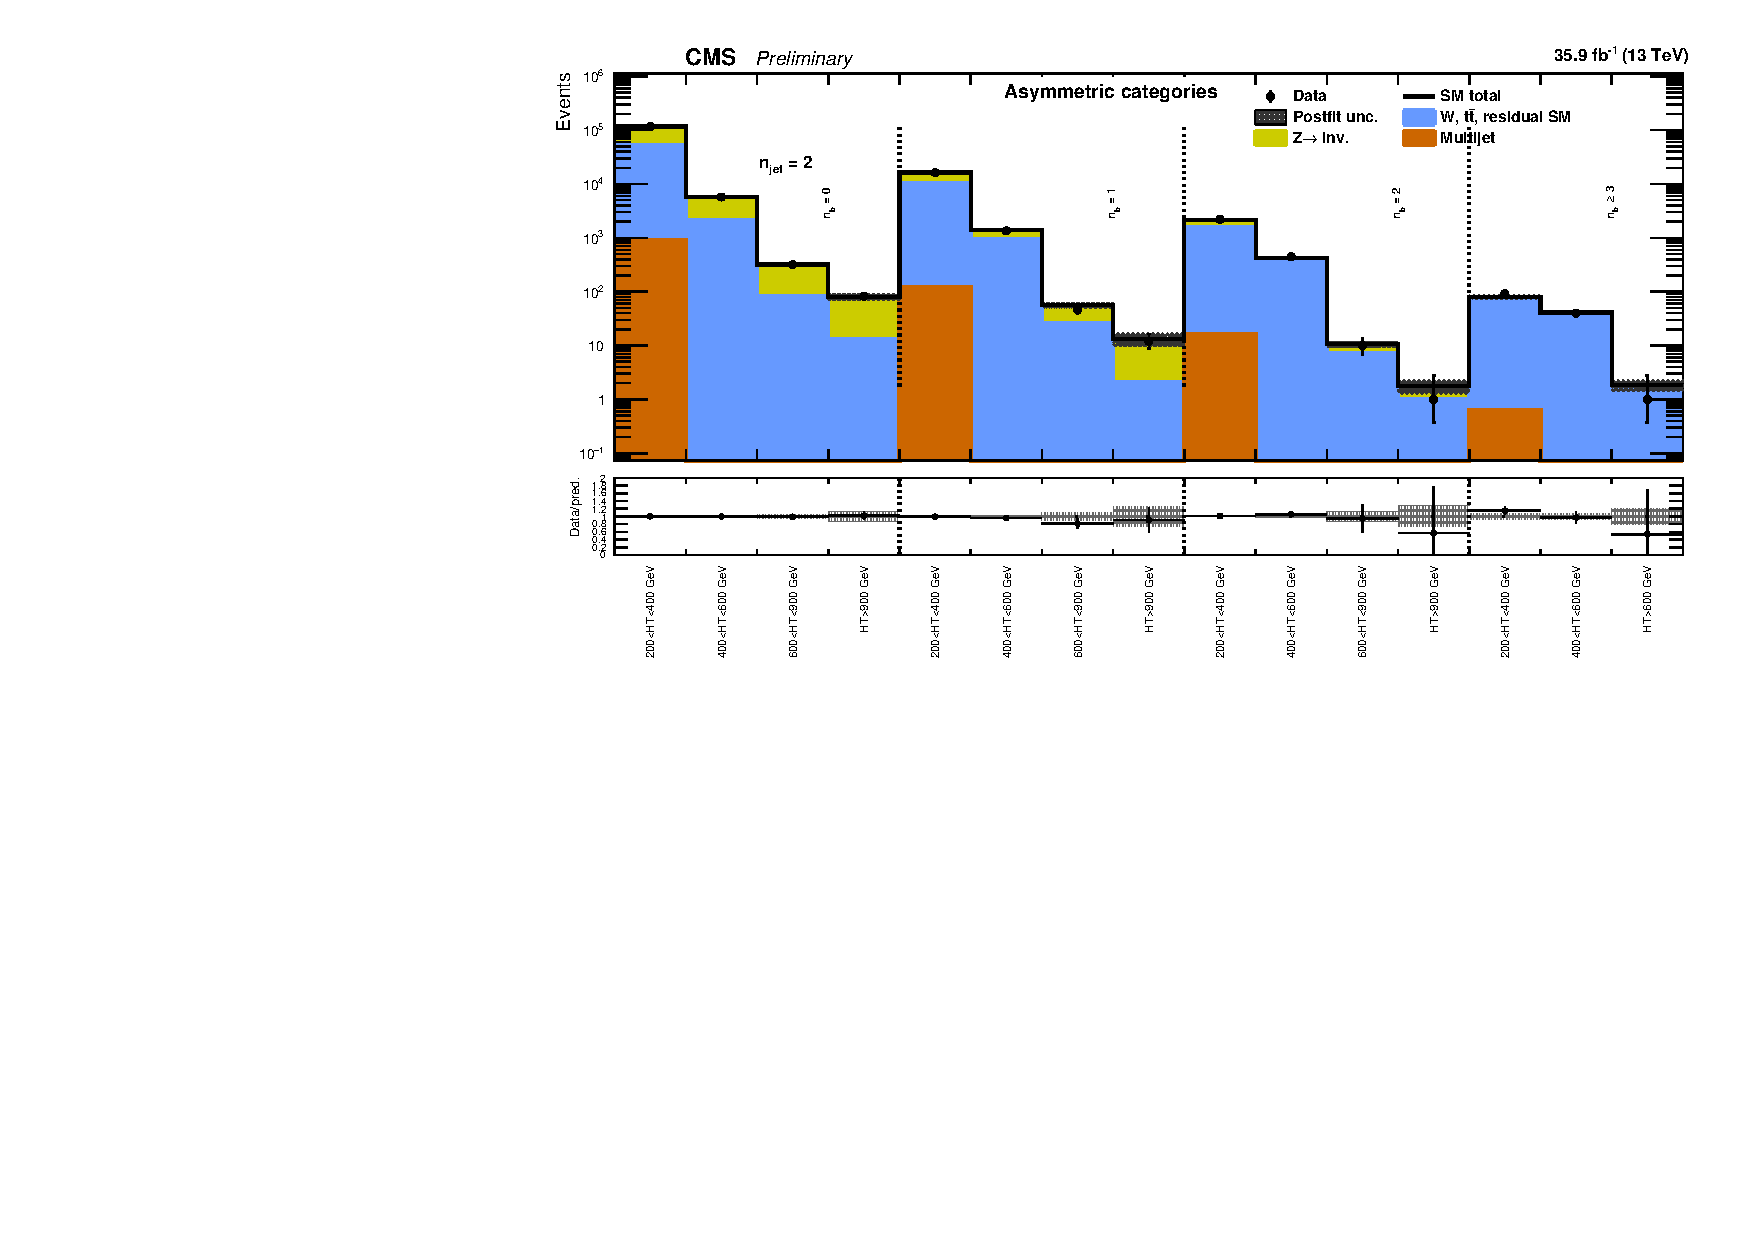
\includegraphics[width=1.\linewidth]{figures/results/36invfb_preapproval/asym/summaryPlot_Asymmetric_fit_b}
\end{figure}

\clearpage
\begin{figure}[h!]
  \centering
  \caption{Upper panel. Event yields observed in data (solid circles)
    and SM expectations with their associated uncertainties (black
    histogram with shaded band) as a function of \nb and \scalht,
    integrated over \mht, and for the asymmetric \njet category
    in the signal region. Lower panel. The pulls, which are obtained
    from both the masked (red markers) and full (blue markers) fits. }
  \label{fig:mr_asym_pulls}
  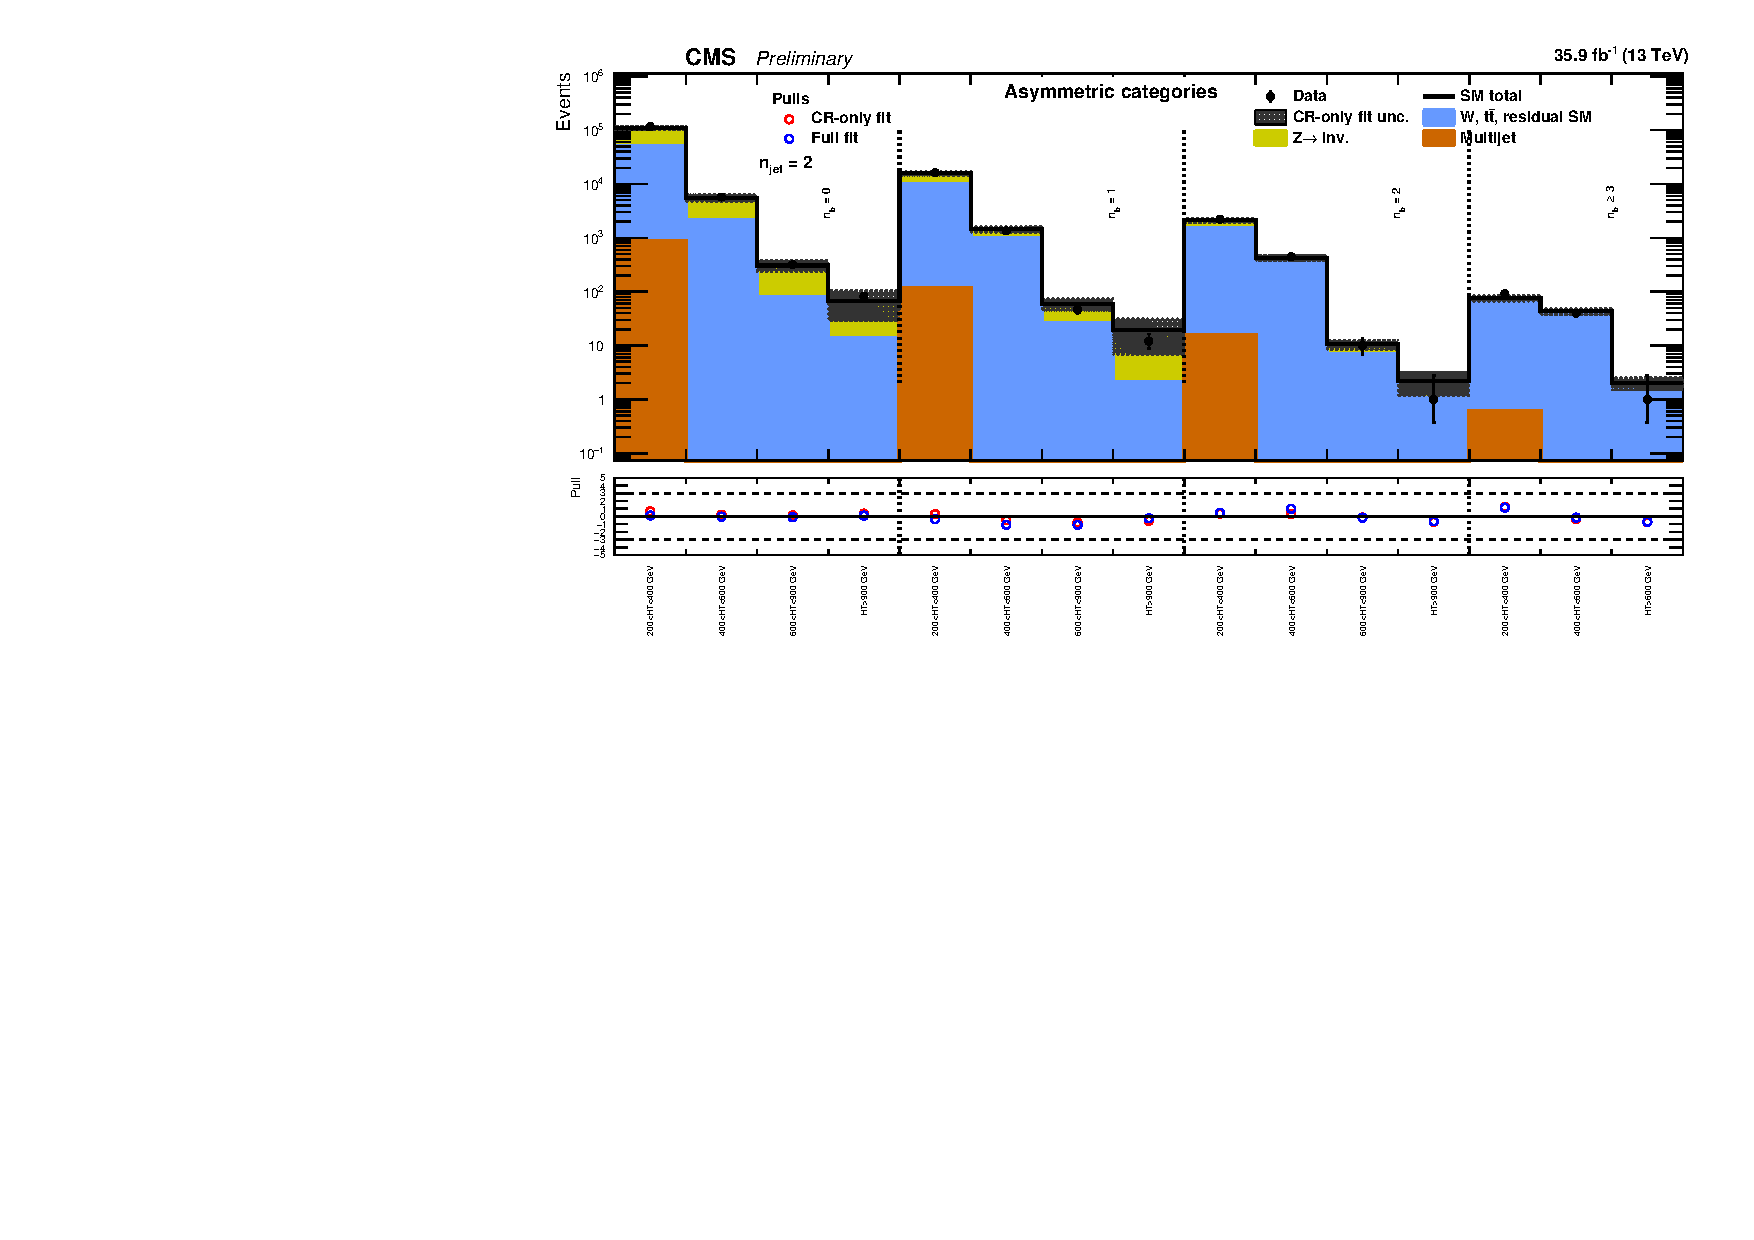
\includegraphics[width=1.\linewidth]{figures/results/36invfb_preapproval/asym/summaryPlot_Asymmetric_prefit_overlay_fit_b}
\end{figure}

\clearpage
\begin{figure}[h!]
  \begin{center}
    \subfigure[$400 < \scalht < 600\GeV$]{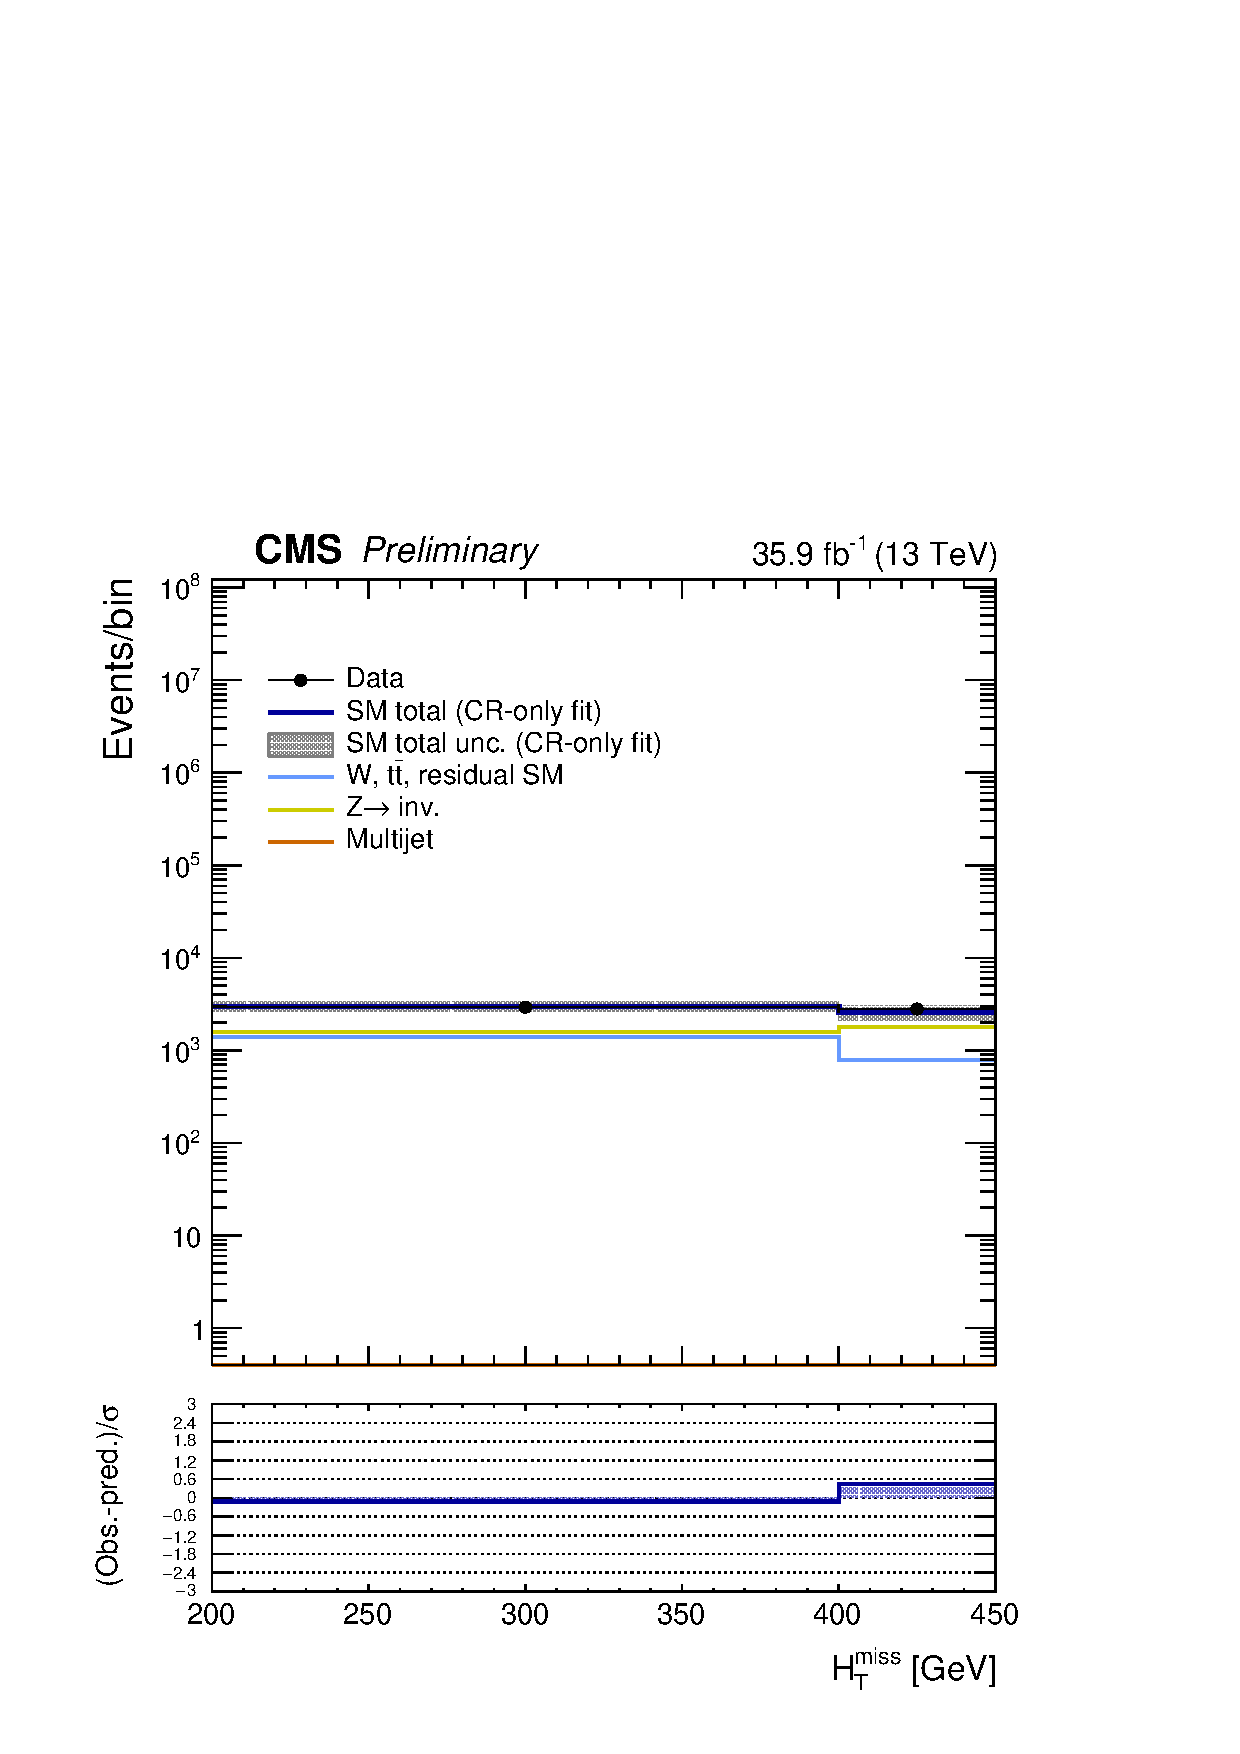
\includegraphics[width=0.49\textwidth]{figures/results/36invfb_preapproval//crfit/shapes//mhtShape_eq0b_ge2a_400_600_crfit.pdf}}
    \subfigure[$600 < \scalht < 900\GeV$]{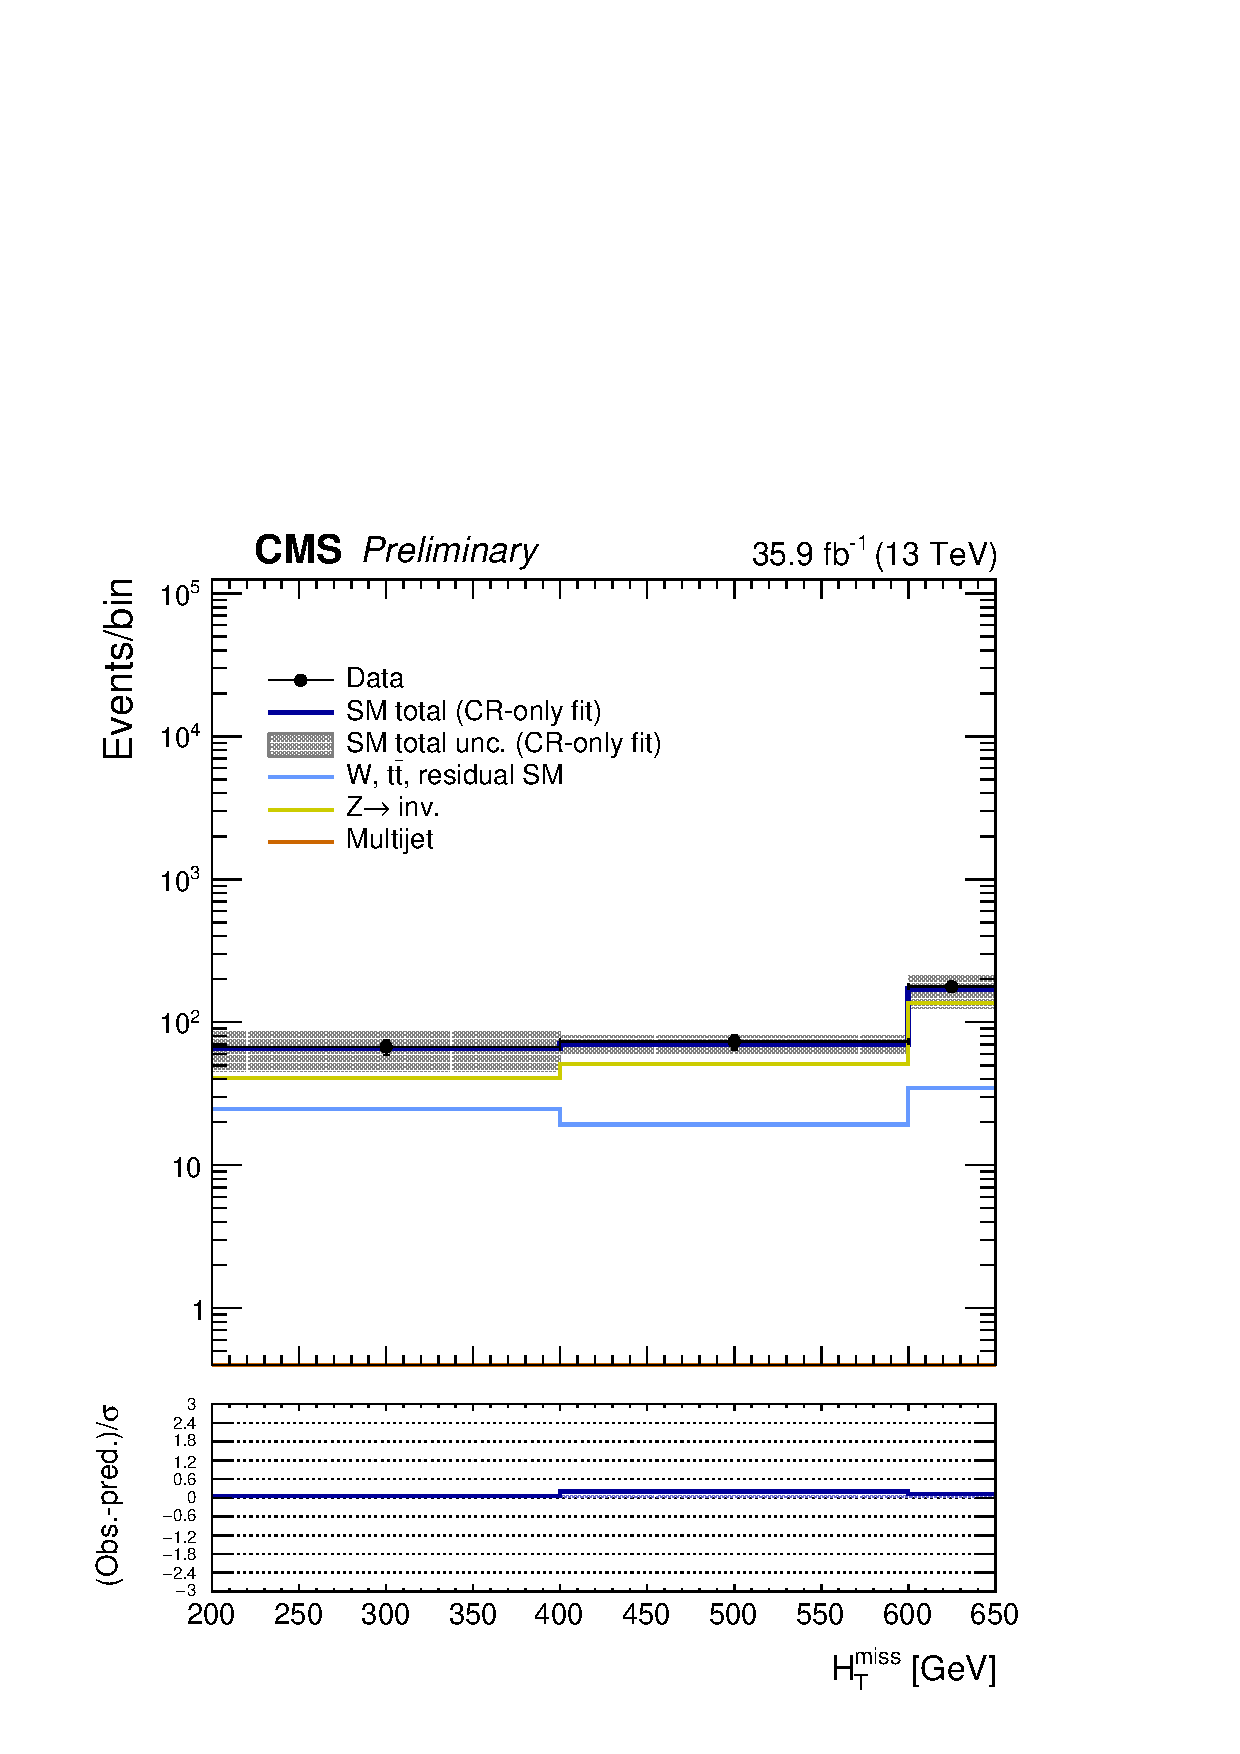
\includegraphics[width=0.49\textwidth]{figures/results/36invfb_preapproval//crfit/shapes//mhtShape_eq0b_ge2a_600_900_crfit.pdf}}\\
    \subfigure[$\scalht > 900\GeV$]{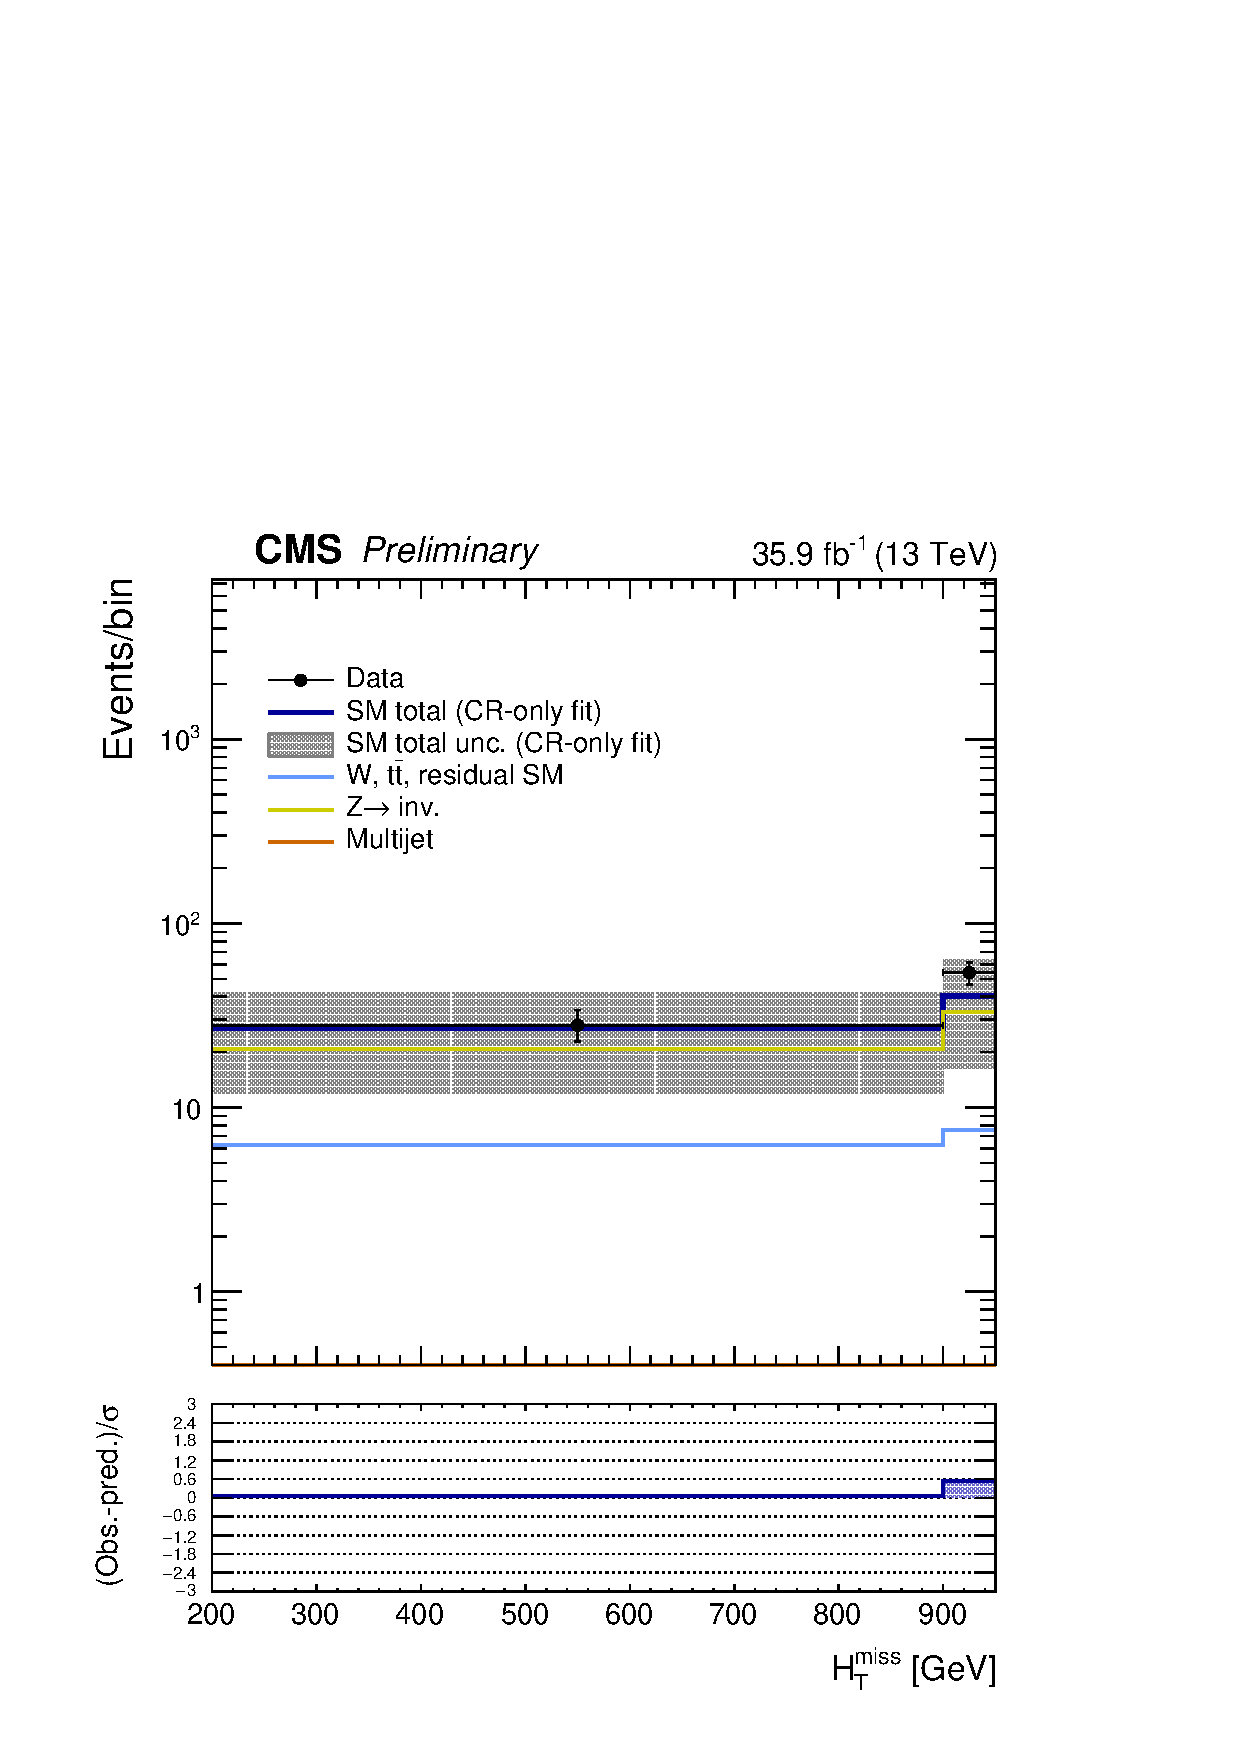
\includegraphics[width=0.49\textwidth]{figures/results/36invfb_preapproval//crfit/shapes//mhtShape_eq0b_ge2a_900_Inf_crfit.pdf}}
    \caption{Event yields observed in data (solid circles) and CR-fit SM expectations with their associated uncertainties (green histogram with shaded band) as a function of \HTmiss based on a sample of events that satisfy $\njet \geq 2 \; \textrm{(asymmetric)}$ and $\nb = 0$, as well as the requirements on \scalht indicated by each sub-figure caption. }
    \label{fig:mhtdim_ge2a_eq0b}
  \end{center}
\end{figure}

\clearpage
\begin{figure}[h!]
  \begin{center}
    \subfigure[$400 < \scalht < 600\GeV$]{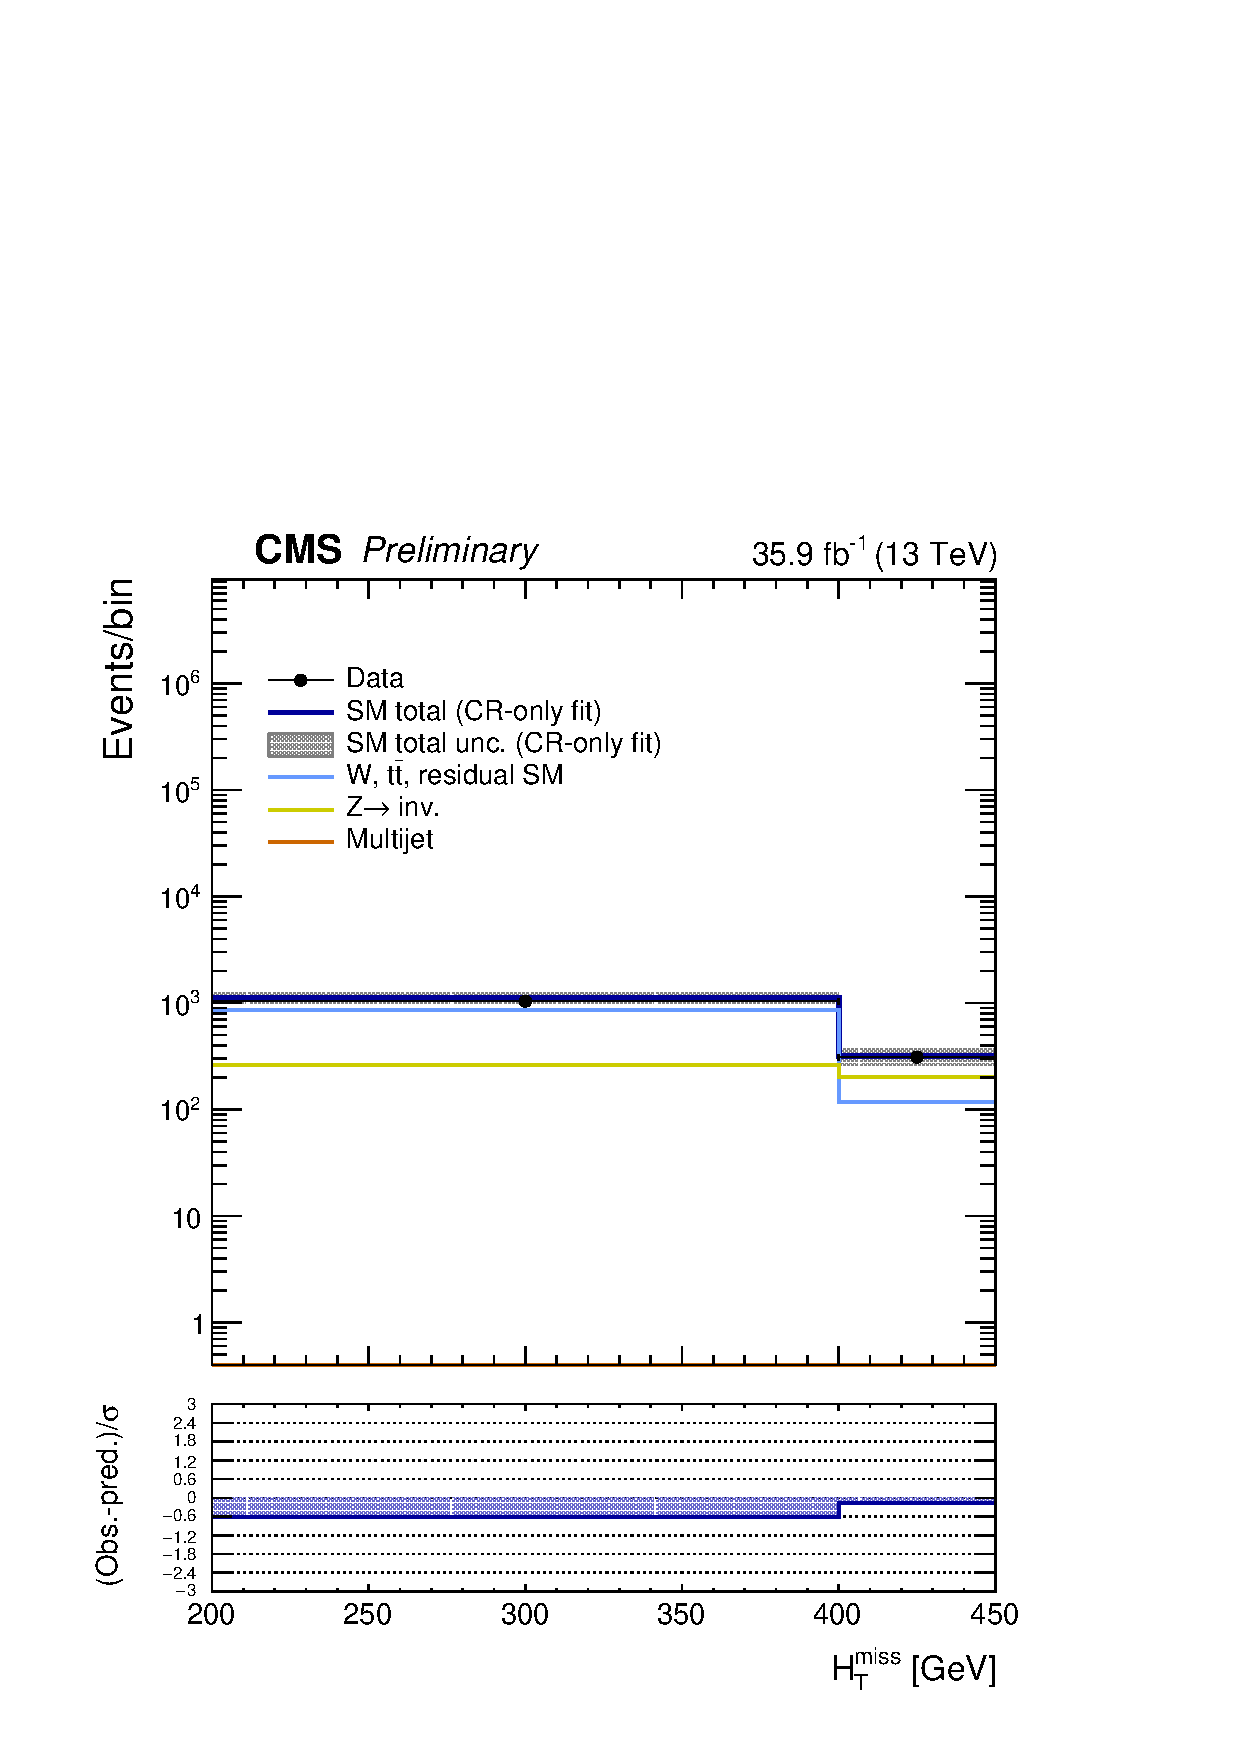
\includegraphics[width=0.49\textwidth]{figures/results/36invfb_preapproval//crfit/shapes//mhtShape_eq1b_ge2a_400_600_crfit.pdf}}
    \subfigure[$600 < \scalht < 900\GeV$]{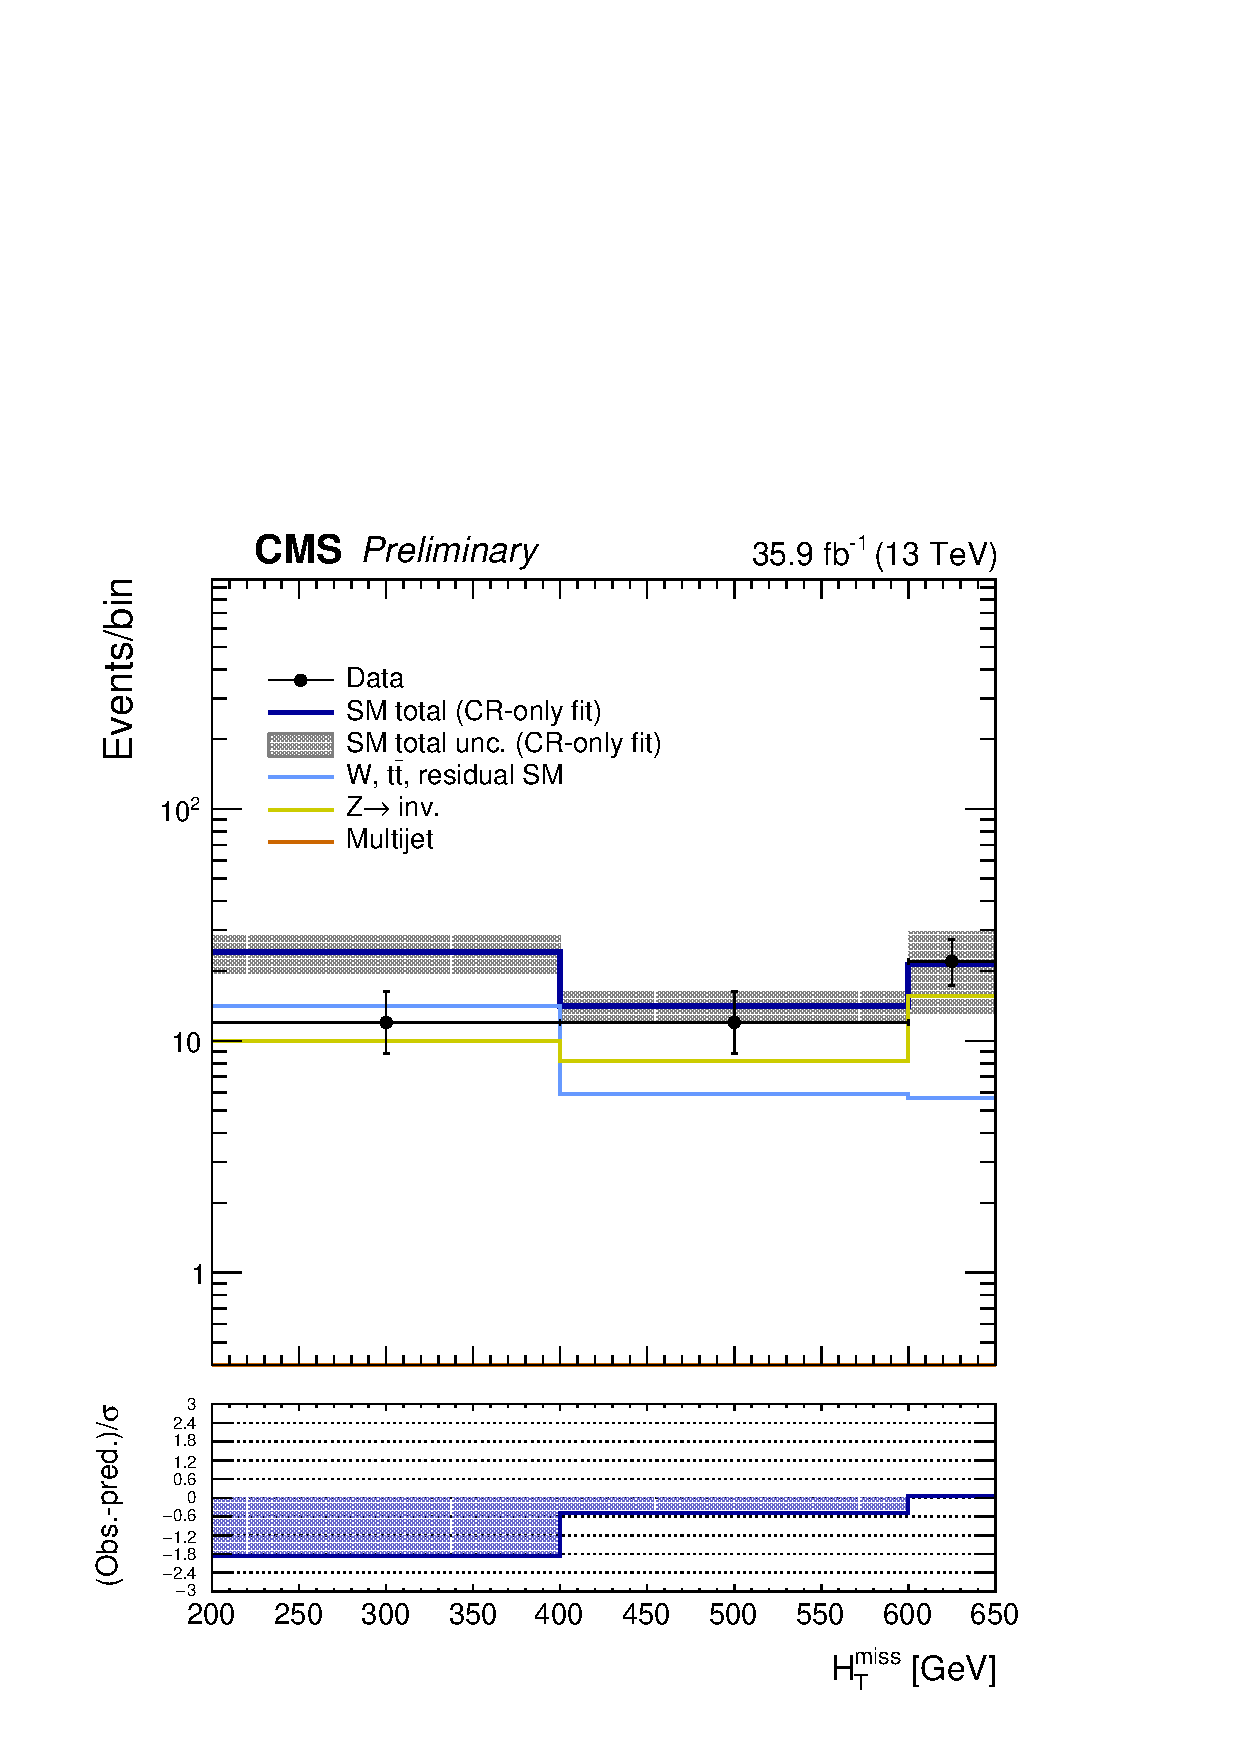
\includegraphics[width=0.49\textwidth]{figures/results/36invfb_preapproval//crfit/shapes//mhtShape_eq1b_ge2a_600_900_crfit.pdf}}\\
    \subfigure[$\scalht > 900\GeV$]{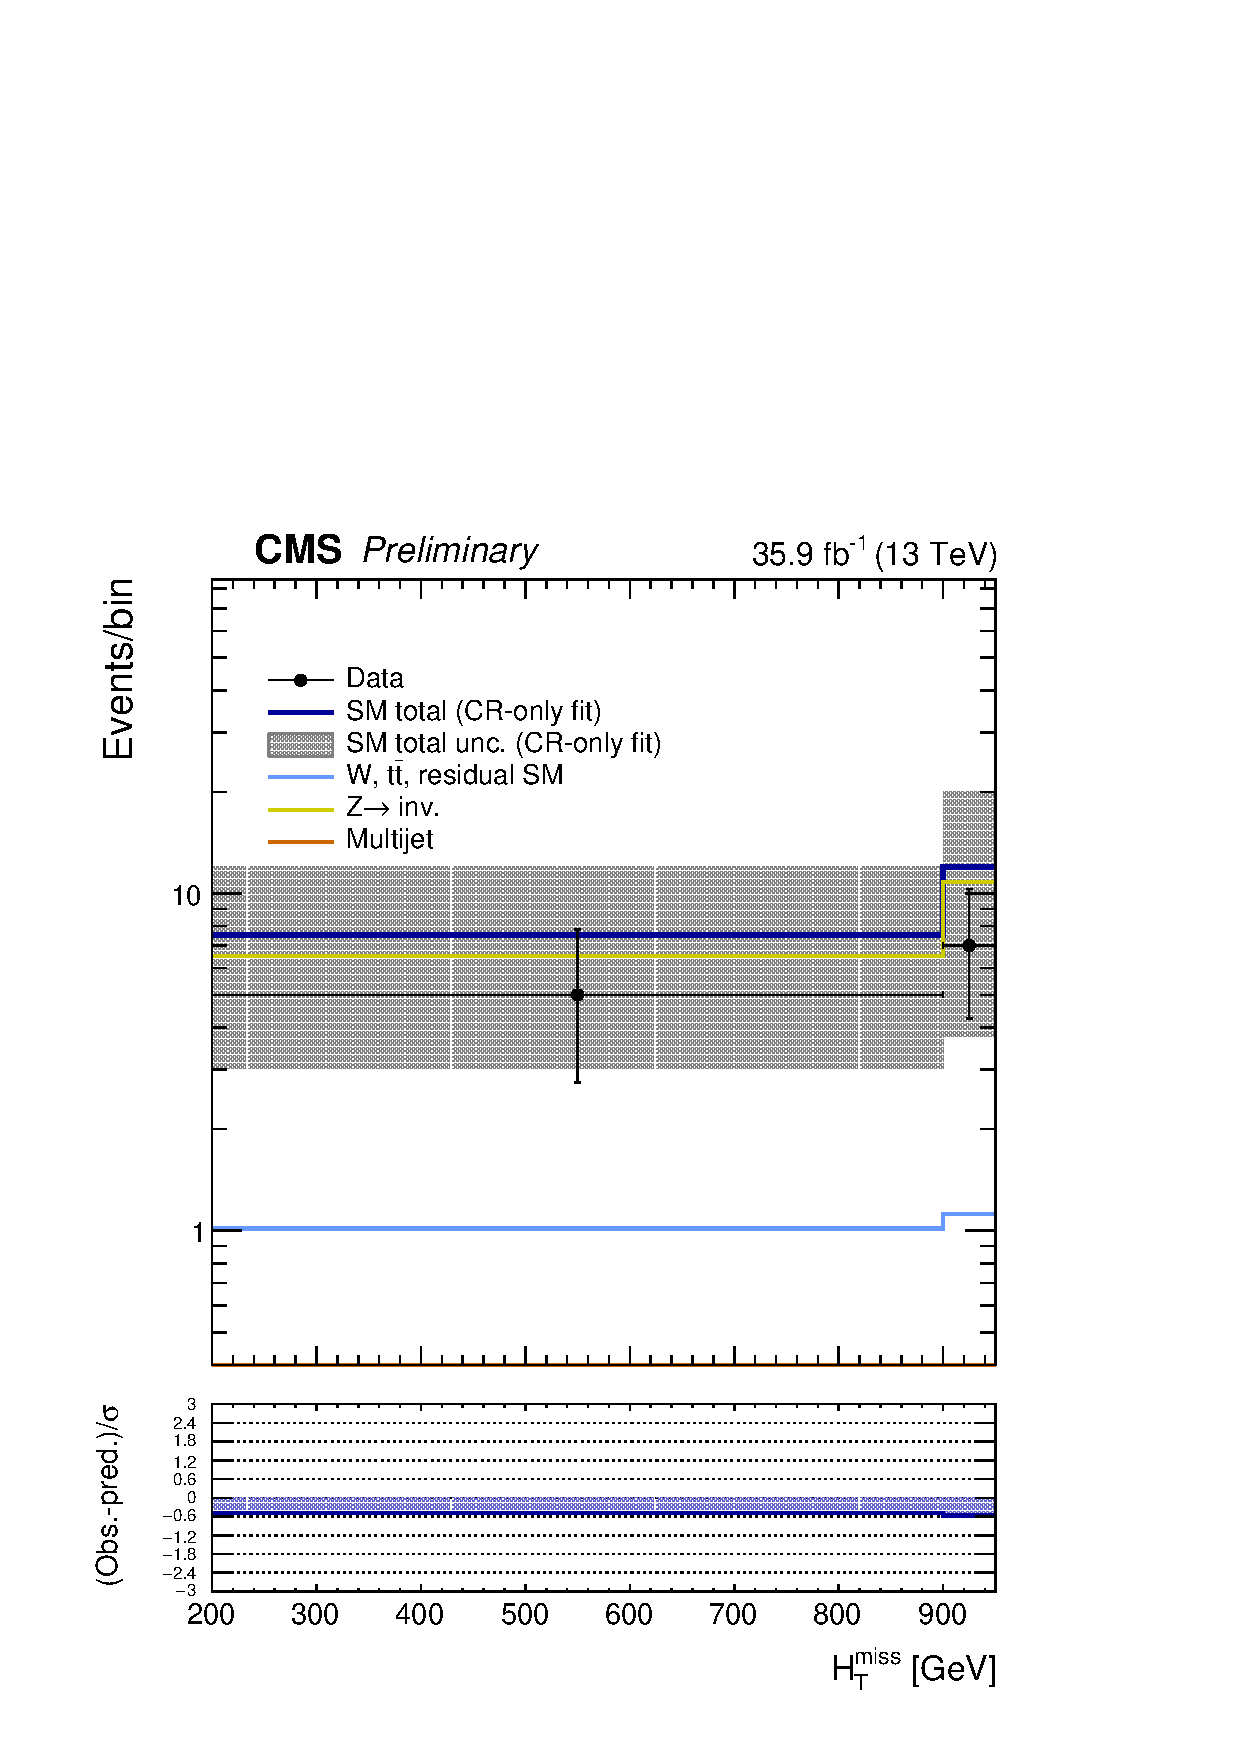
\includegraphics[width=0.49\textwidth]{figures/results/36invfb_preapproval//crfit/shapes//mhtShape_eq1b_ge2a_900_Inf_crfit.pdf}}
    \caption{Event yields observed in data (solid circles) and CR-fit SM expectations with their associated uncertainties (green histogram with shaded band) as a function of \HTmiss based on a sample of events that satisfy $\njet \geq 2 \; \textrm{(asymmetric)}$ and $\nb = 1$, as well as the requirements on \scalht indicated by each sub-figure caption. }
    \label{fig:mhtdim_ge2a_eq1b}
  \end{center}
\end{figure}

\clearpage
\begin{figure}[h!]
  \begin{center}
    \subfigure[$400 < \scalht < 600\GeV$]{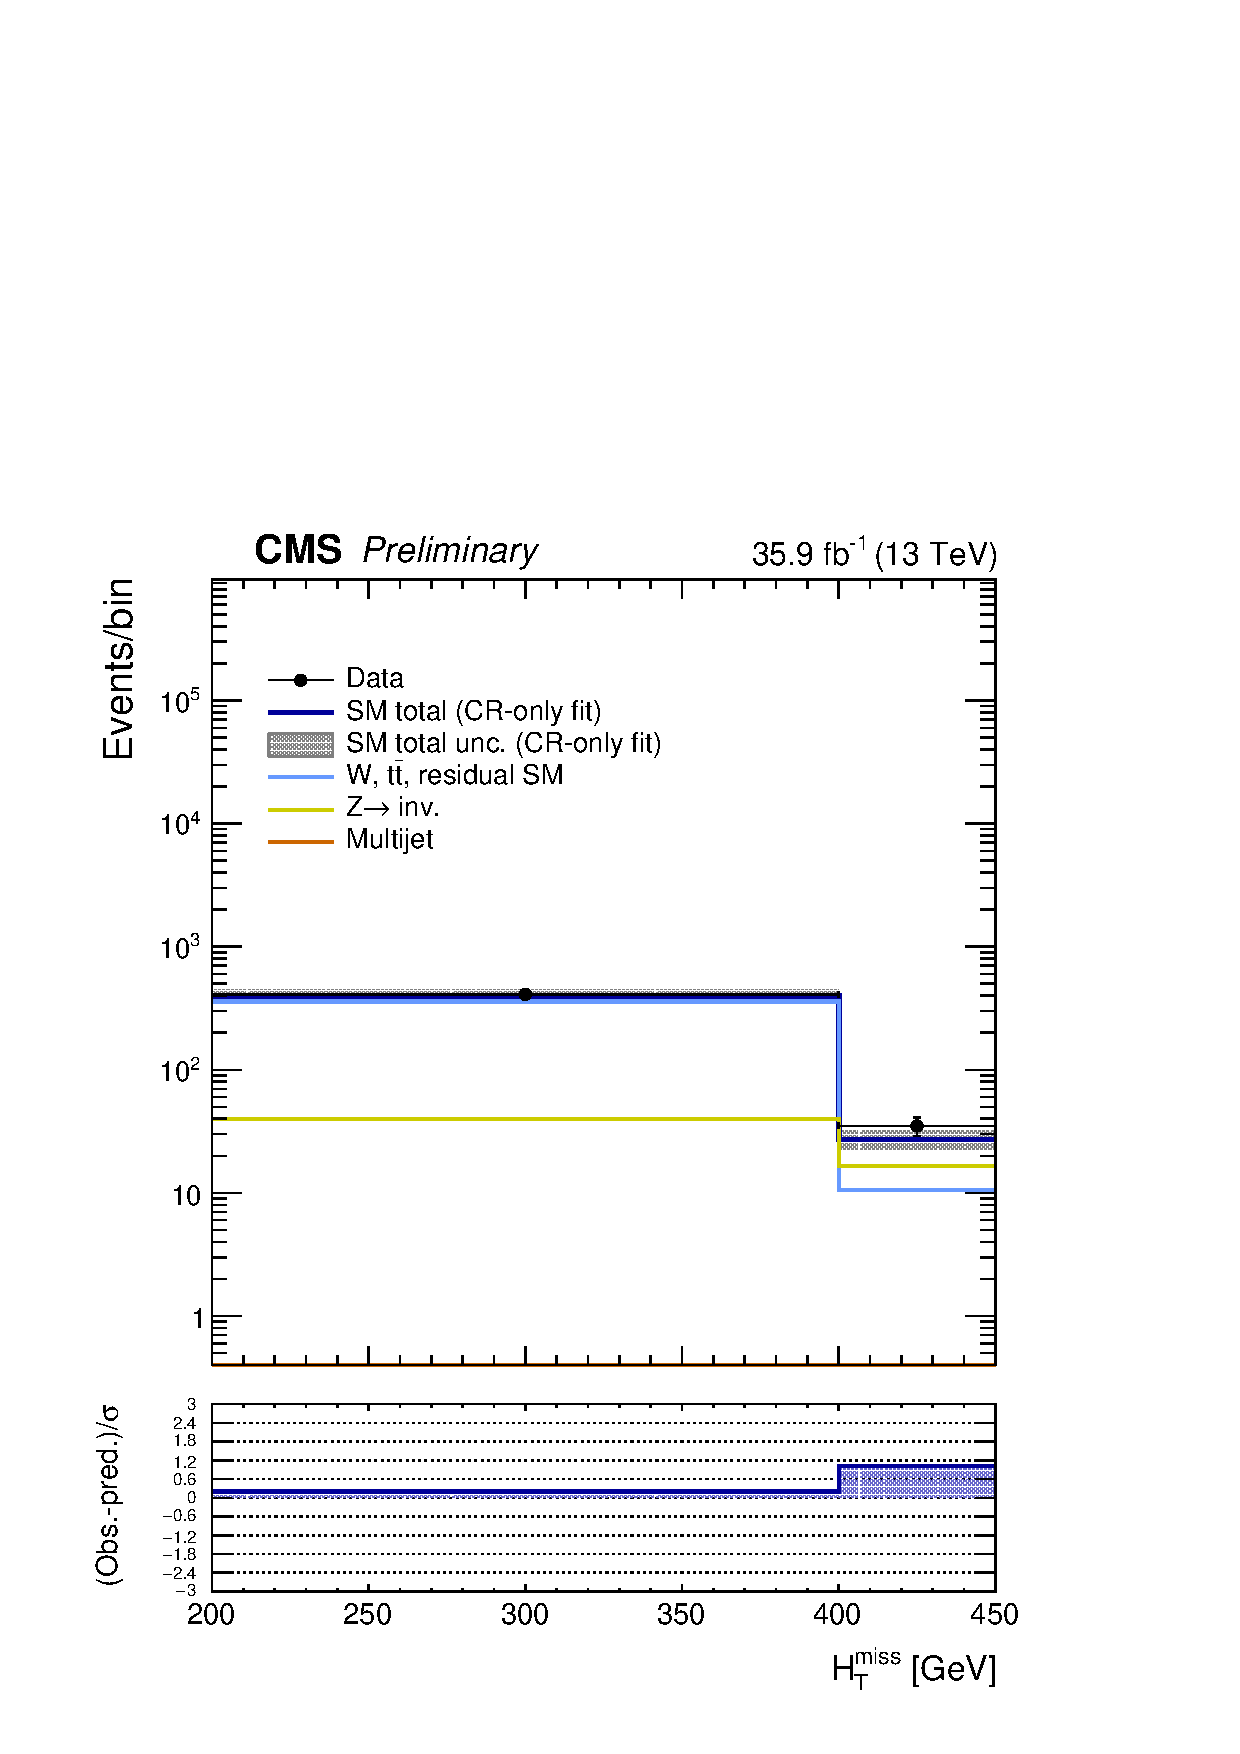
\includegraphics[width=0.49\textwidth]{figures/results/36invfb_preapproval//crfit/shapes//mhtShape_eq2b_ge2a_400_600_crfit.pdf}}
    \subfigure[$600 < \scalht < 900\GeV$]{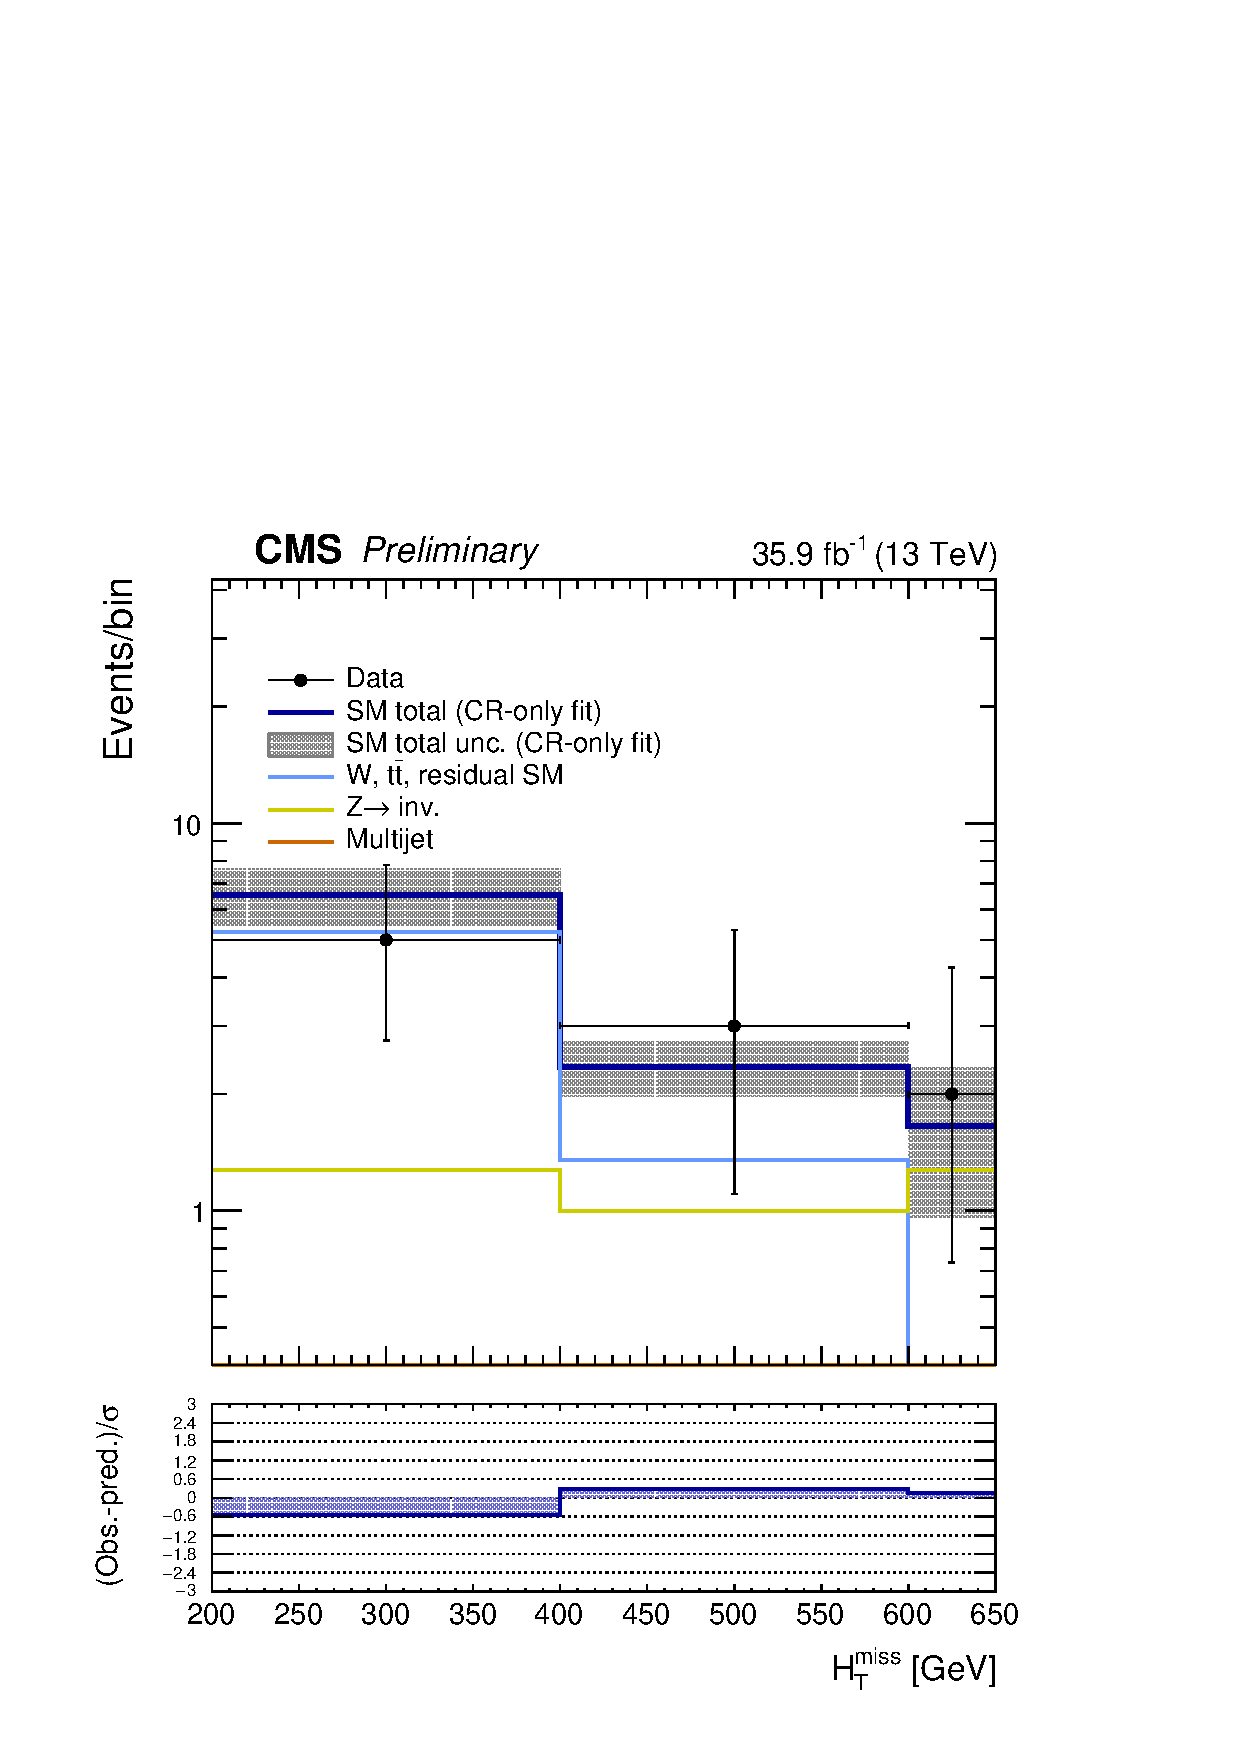
\includegraphics[width=0.49\textwidth]{figures/results/36invfb_preapproval//crfit/shapes//mhtShape_eq2b_ge2a_600_900_crfit.pdf}}\\
    \subfigure[$\scalht > 900\GeV$]{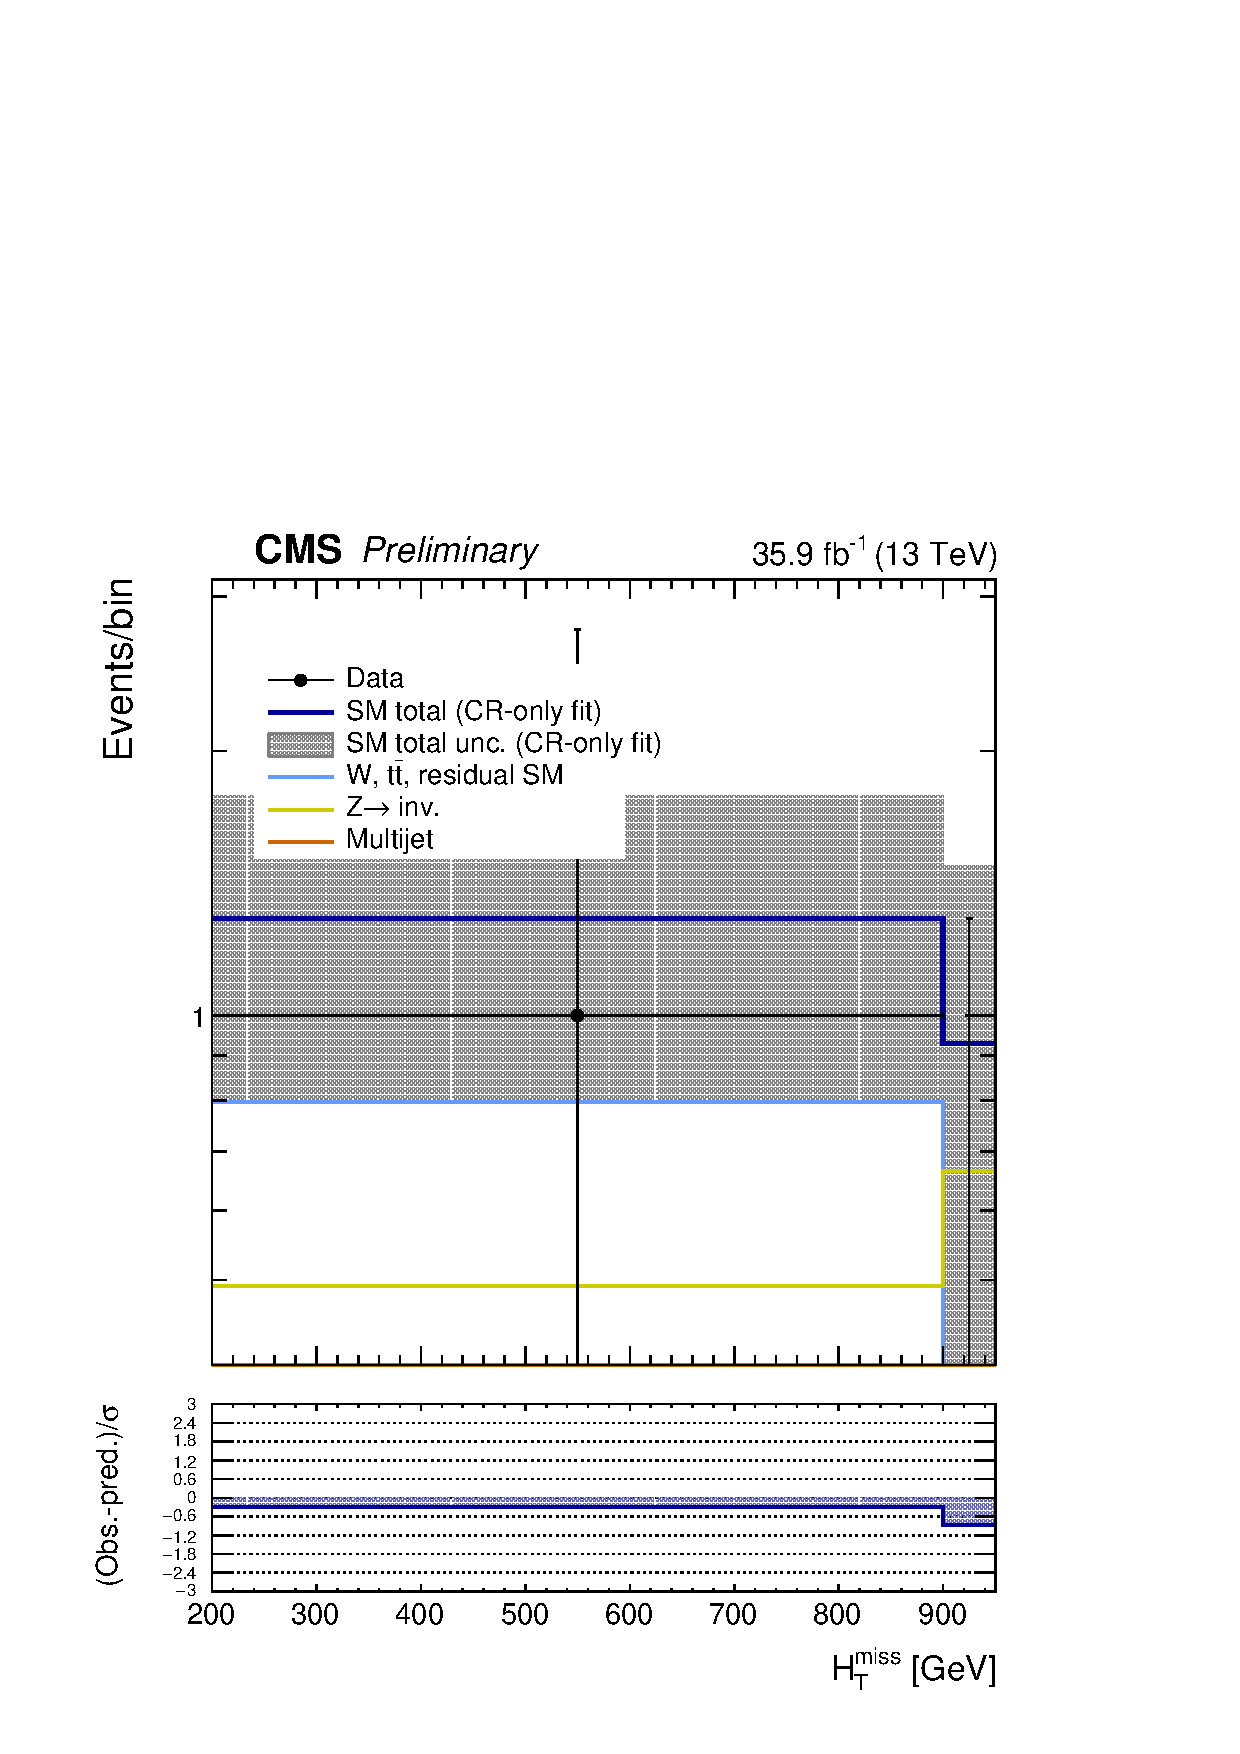
\includegraphics[width=0.49\textwidth]{figures/results/36invfb_preapproval//crfit/shapes//mhtShape_eq2b_ge2a_900_Inf_crfit.pdf}}
    \caption{Event yields observed in data (solid circles) and CR-fit SM expectations with their associated uncertainties (green histogram with shaded band) as a function of \HTmiss based on a sample of events that satisfy $\njet \geq 2 \; \textrm{(asymmetric)}$ and $\nb = 2$, as well as the requirements on \scalht indicated by each sub-figure caption. }
    \label{fig:mhtdim_ge2a_eq2b}
  \end{center}
\end{figure}

\clearpage
\subsection{Symmetric topology}
\label{app:results-orig-symm}

Figures~\ref{fig:mr_symm_pre} and \ref{fig:mr_symm_post} summarise the
event yields observed in data and SM expectations with their
associated uncertainties as a function of \scalht and \nb, {\it
  integated over \mht}, for the monojet category ($\njet = 1$) for the
masked and full fits, respectively. The lower panels show the
data-to-background ratios for the masked and full fits.
Figure~\ref{fig:mr_symm_pulls} shows background expectations for the
masked fit in the upper panel, as shown in Fig.~\ref{fig:mr_symm_pre},
and the pulls (\ie the difference between data and the background
estimates relative to their uncertainties) for both the masked and
full fits in the lower panel.

Figures~\ref{fig:mhtdim_eq2j_eq0b}--\ref{fig:mhtdim_ge6j_eq3b}
summarise the observed event yields and CR-fit SM expectations with
their associated uncertainties as a function of \HTmiss for based on a
sample of events that satisfy requirements on \njet (symmetric), \nb
and \scalht.

\clearpage
\begin{figure}[h!]
  \centering
  \caption{Upper panel. Event yields observed in data (solid circles)
    and SM expectations with their associated uncertainties (black
    histogram with shaded band) as a function of \nb and \scalht,
    integrated over \mht, and for the symmmetric \njet category
    in the signal region. Lower panel. Data-to-background ratios. The
    background estimates and ratios are from the masked fit. }
  \label{fig:mr_symm_pre}
  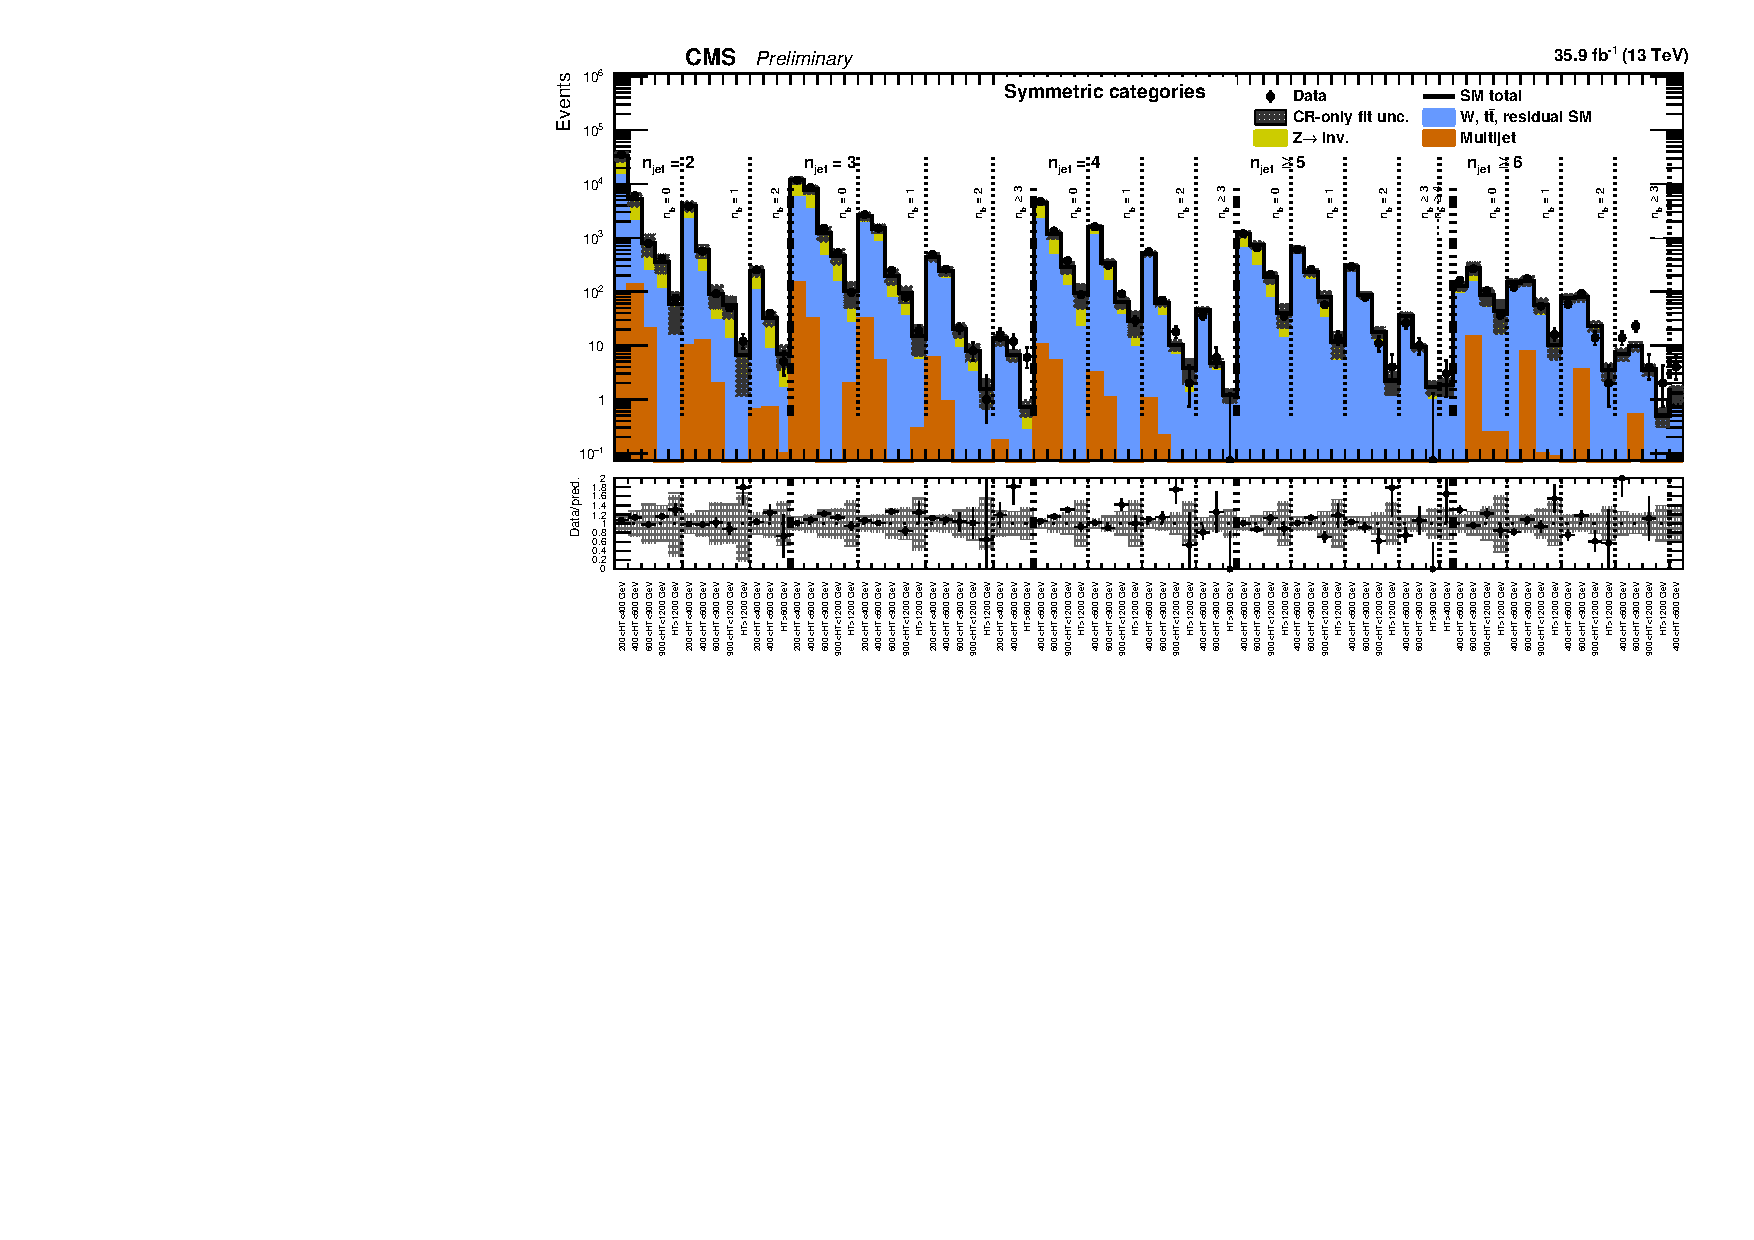
\includegraphics[width=1.\linewidth]{figures/results/36invfb_preapproval/symm/summaryPlot_Symmetric_prefit}
\end{figure}

\clearpage
\begin{figure}[h!]
  \centering
  \caption{Upper panel. Event yields observed in data (solid circles)
    and SM expectations with their associated uncertainties (black
    histogram with shaded band) as a function of \nb and \scalht,
    integrated over \mht, and for the symmmetric \njet category
    in the signal region. Lower panel. Data-to-background ratios. The
    background estimates and ratios are obtained with the full fit. }
  \label{fig:mr_symm_post}
  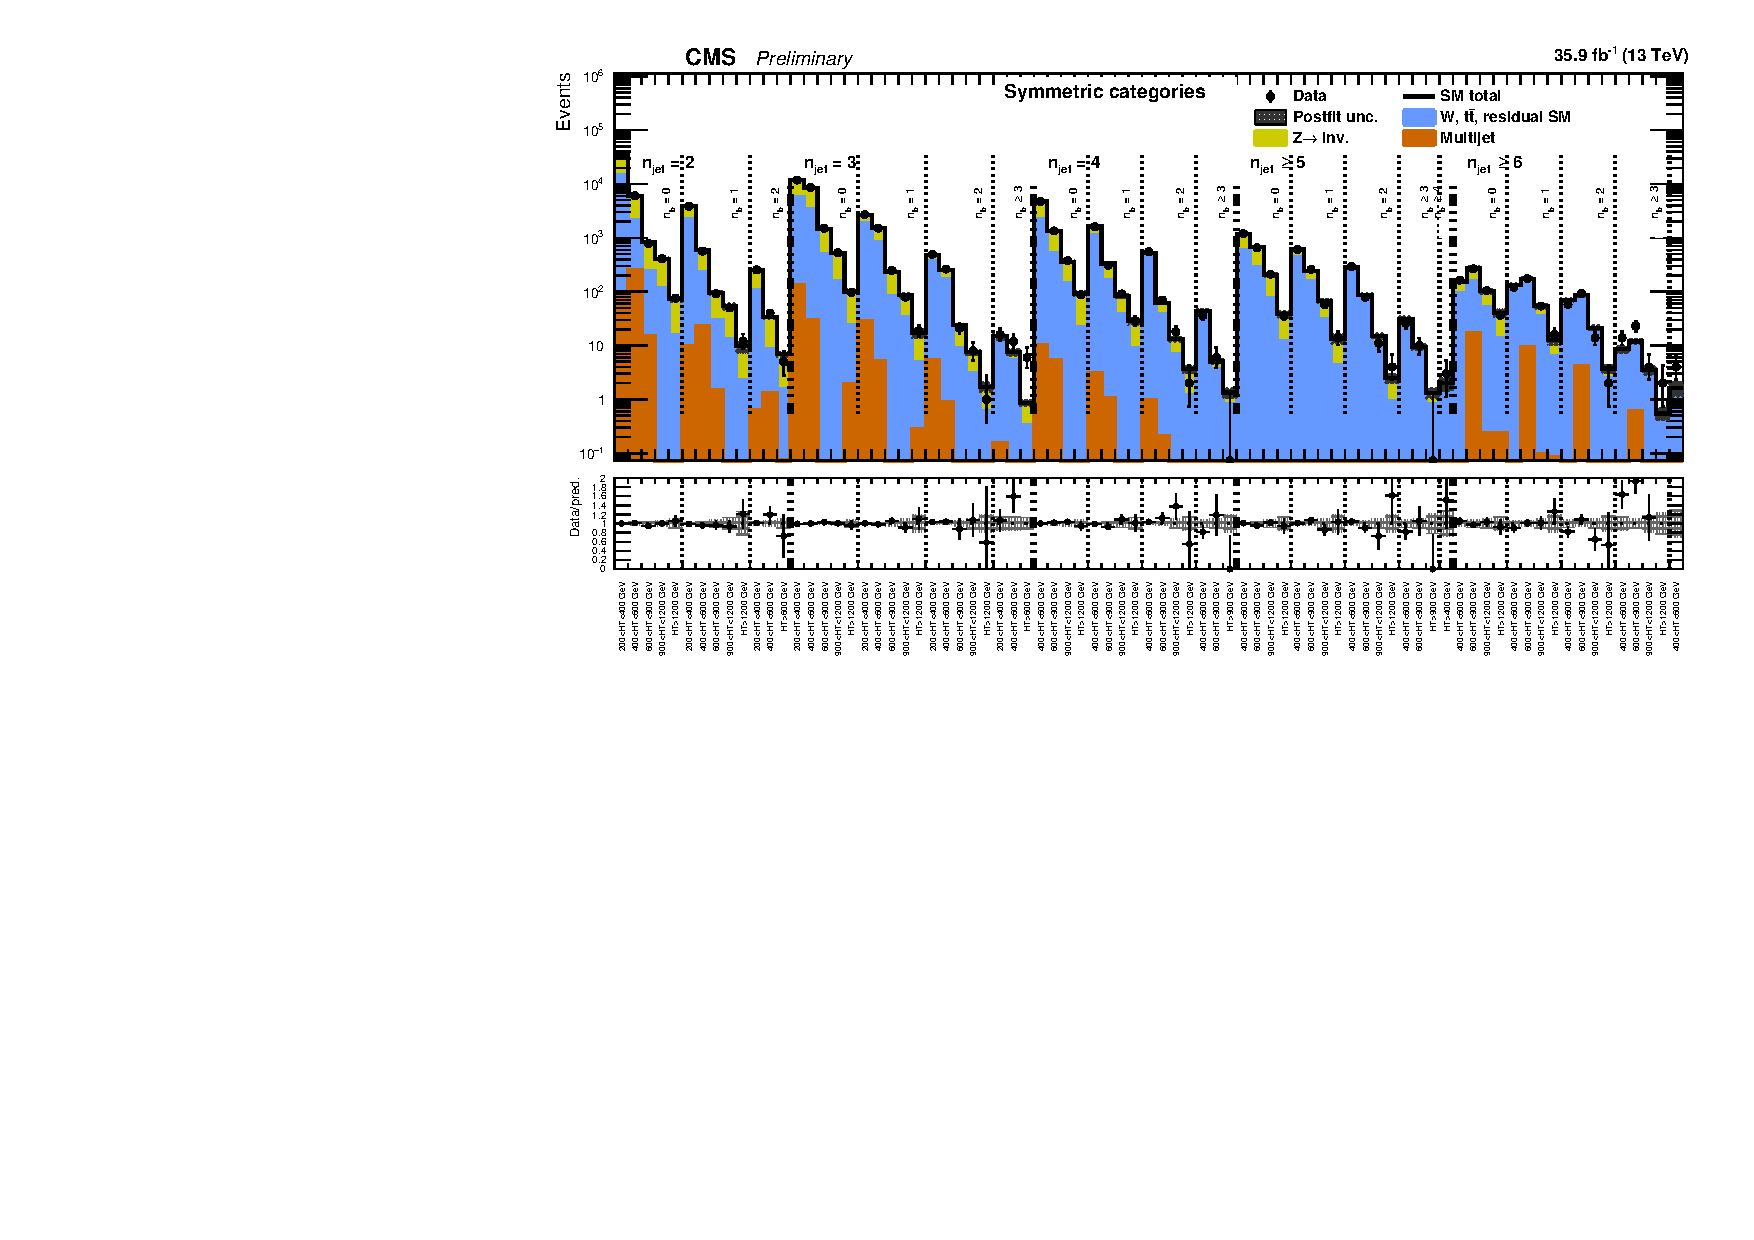
\includegraphics[width=1.\linewidth]{figures/results/36invfb_preapproval/symm/summaryPlot_Symmetric_fit_b}
\end{figure}

\clearpage
\begin{figure}[h!]
  \centering
  \caption{Upper panel. Event yields observed in data (solid circles)
    and SM expectations with their associated uncertainties (black
    histogram with shaded band) as a function of \nb and \scalht,
    integrated over \mht, and for the symmmetric \njet category
    in the signal region. Lower panel. The pulls, which are obtained
    from both the masked (red markers) and full (blue markers) fits. }
  \label{fig:mr_symm_pulls}
  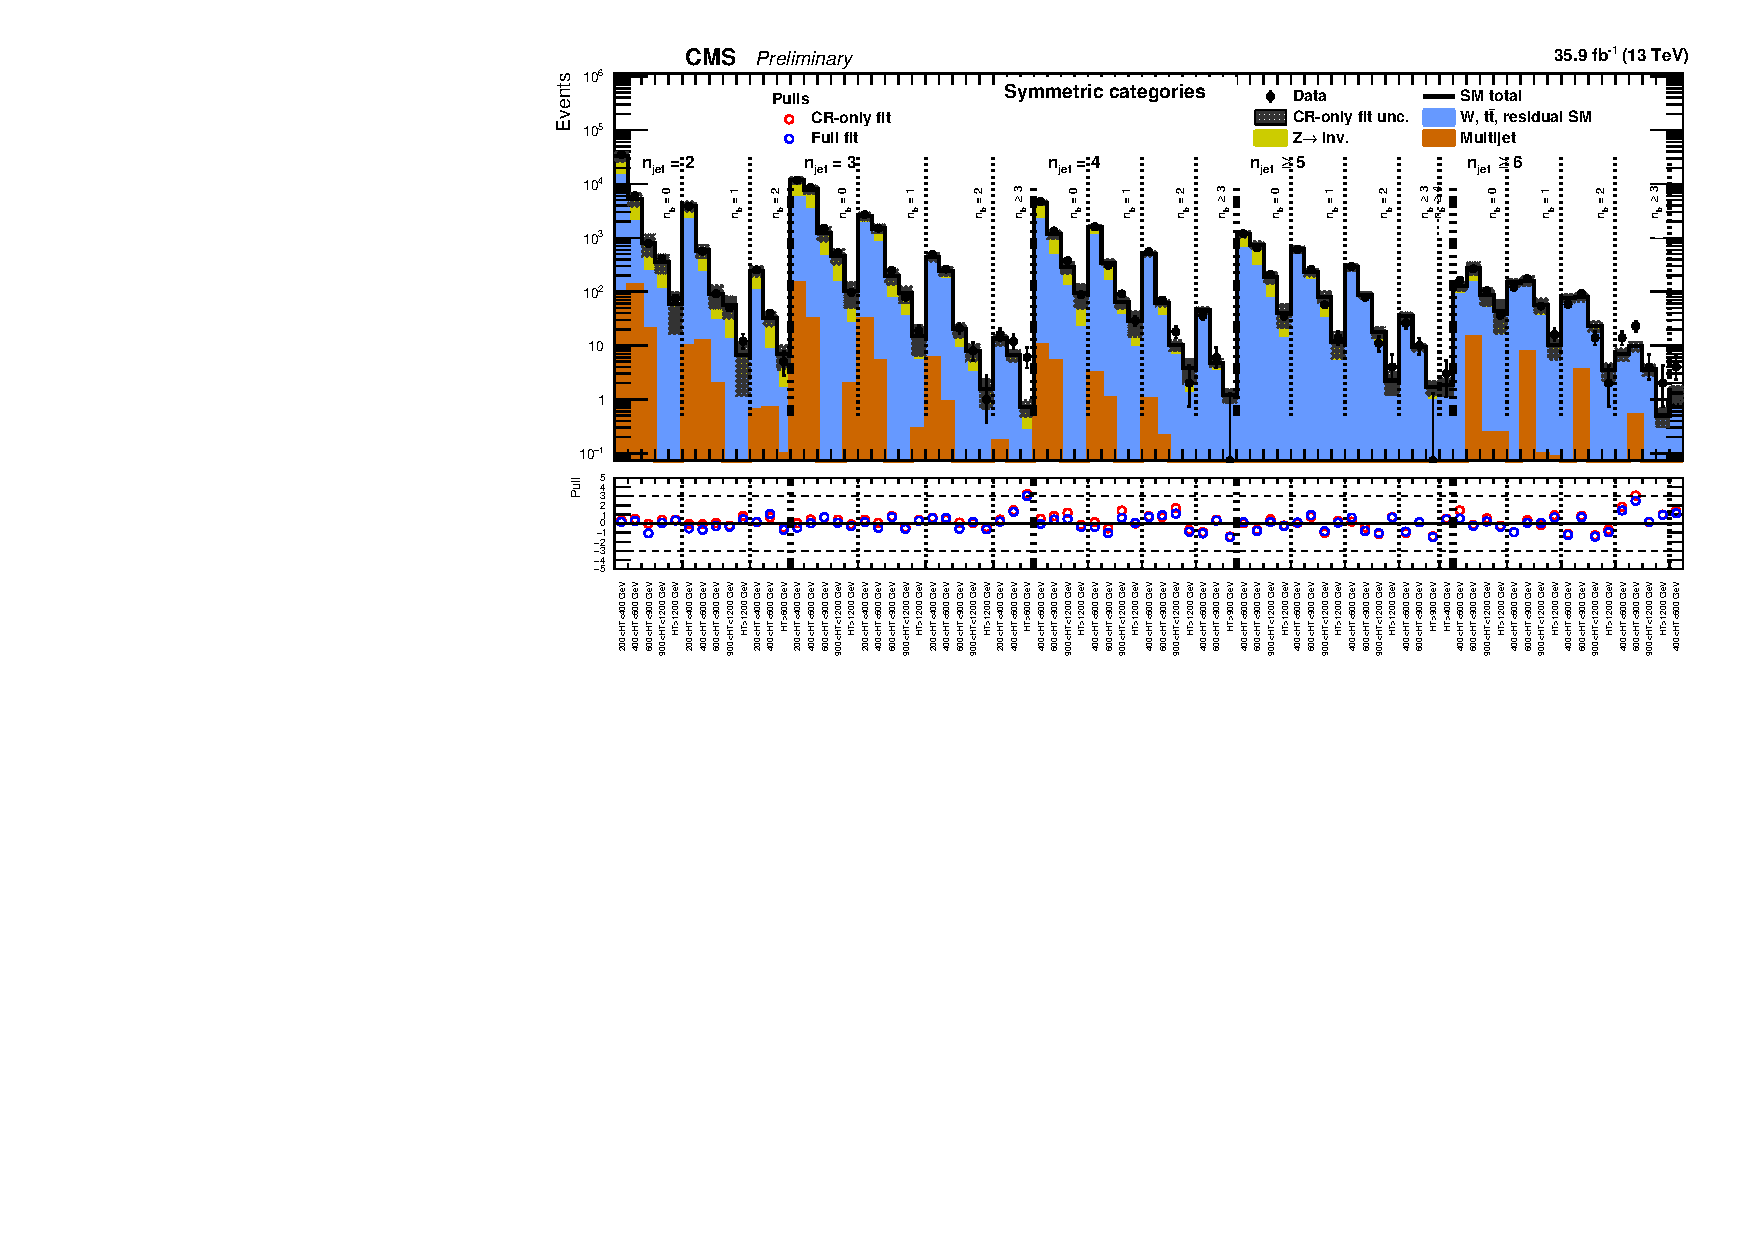
\includegraphics[width=1.\linewidth]{figures/results/36invfb_preapproval/symm/summaryPlot_Symmetric_prefit_overlay_fit_b}
\end{figure}

\clearpage
\begin{figure}[h!]
  \begin{center}
    \subfigure[$400 < \scalht < 600\GeV$]{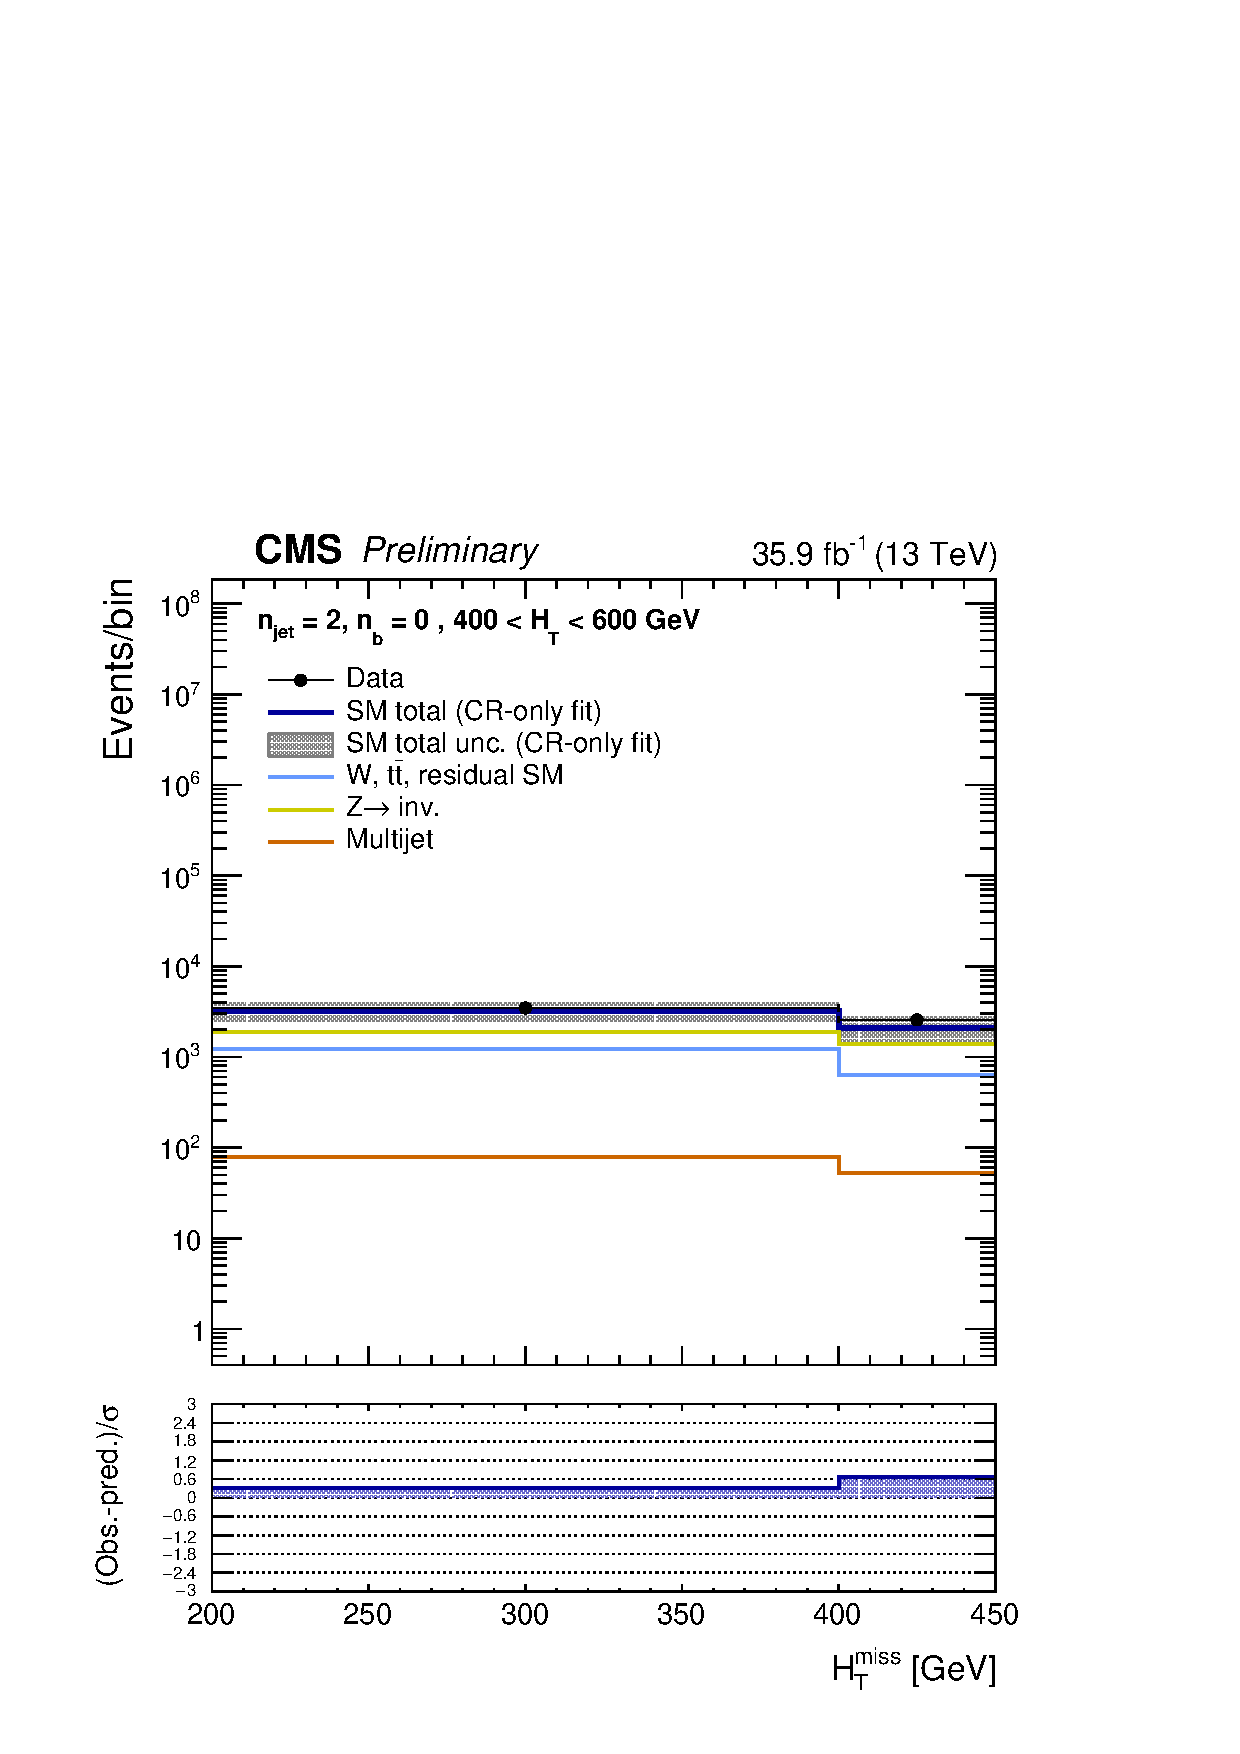
\includegraphics[width=0.49\textwidth]{figures/results/36invfb_preapproval//crfit/shapes//mhtShape_eq0b_eq2j_400_600_crfit.pdf}}
    \subfigure[$600 < \scalht < 900\GeV$]{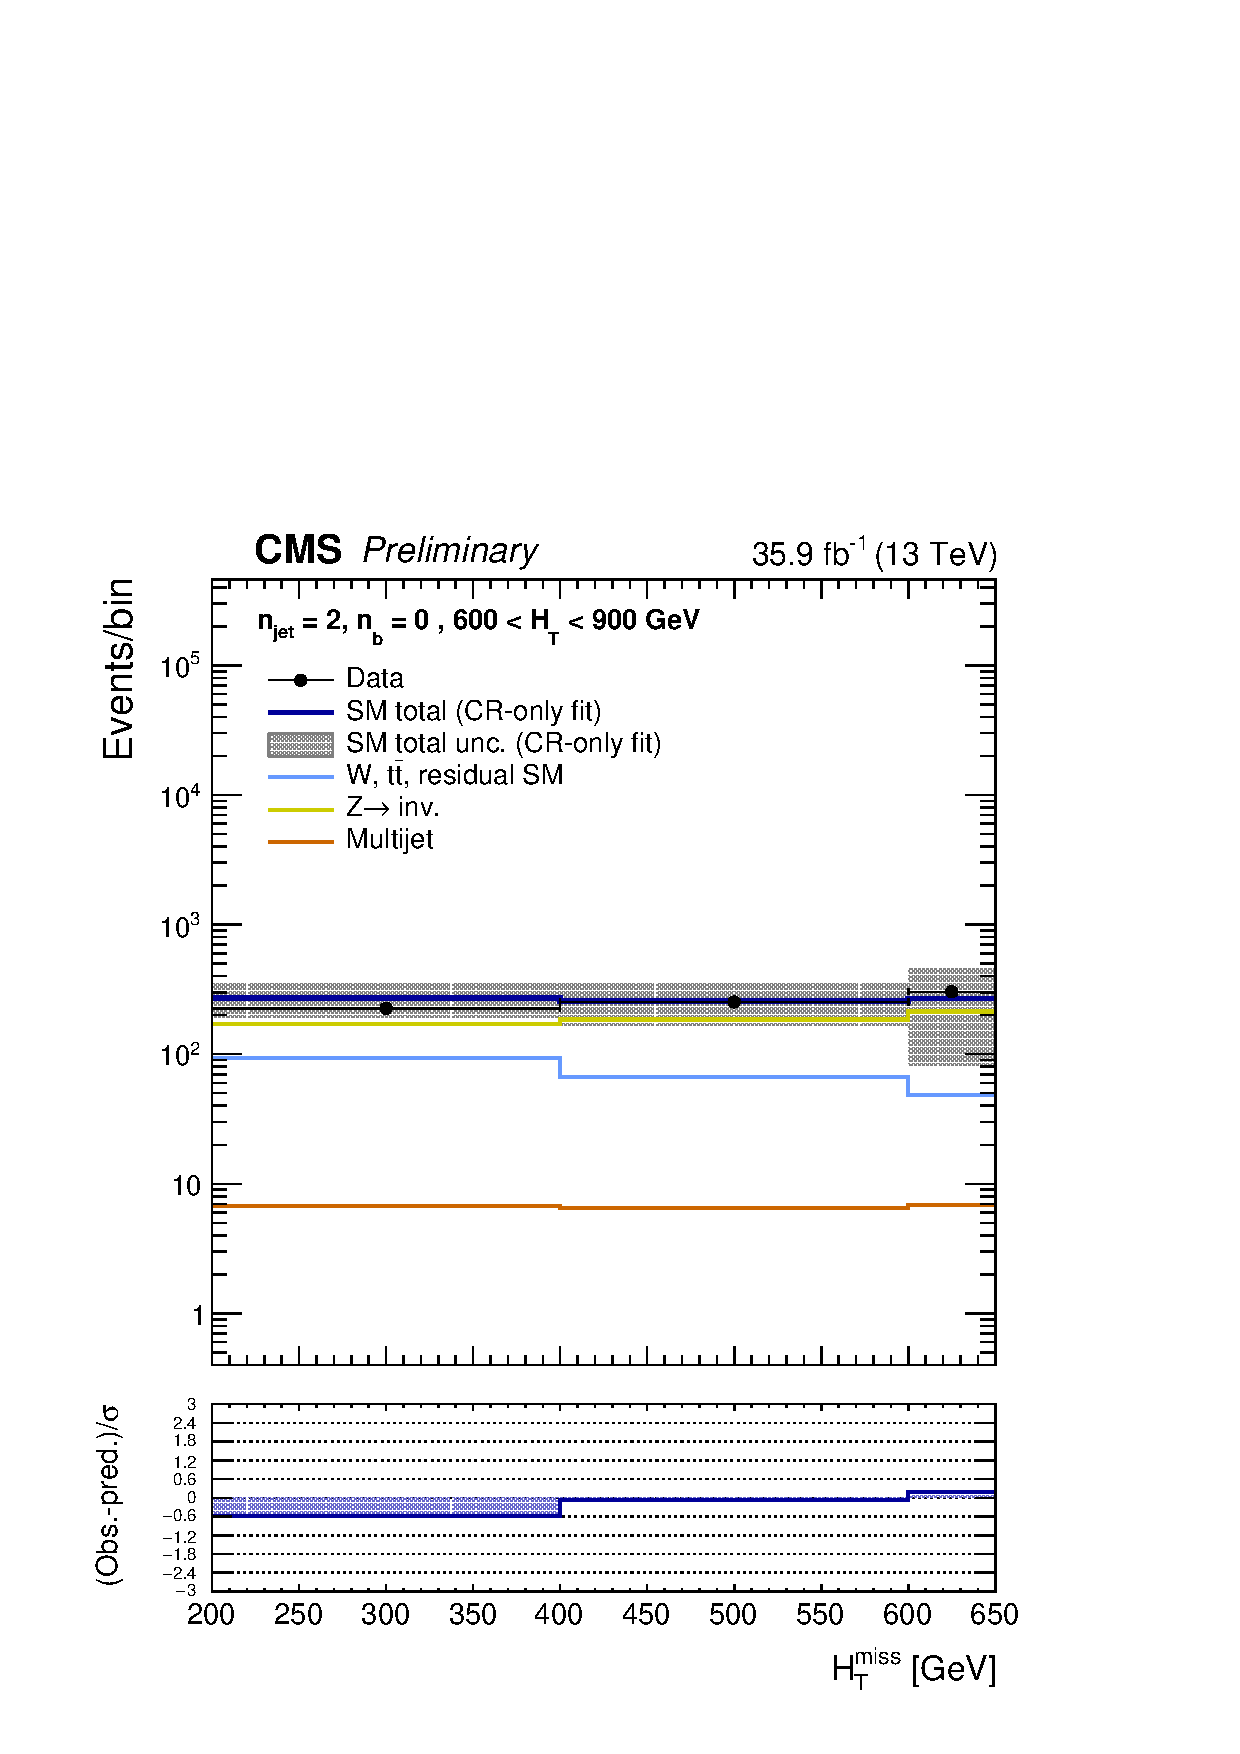
\includegraphics[width=0.49\textwidth]{figures/results/36invfb_preapproval//crfit/shapes//mhtShape_eq0b_eq2j_600_900_crfit.pdf}}\\
    \subfigure[$900 < \scalht < 1200\GeV$]{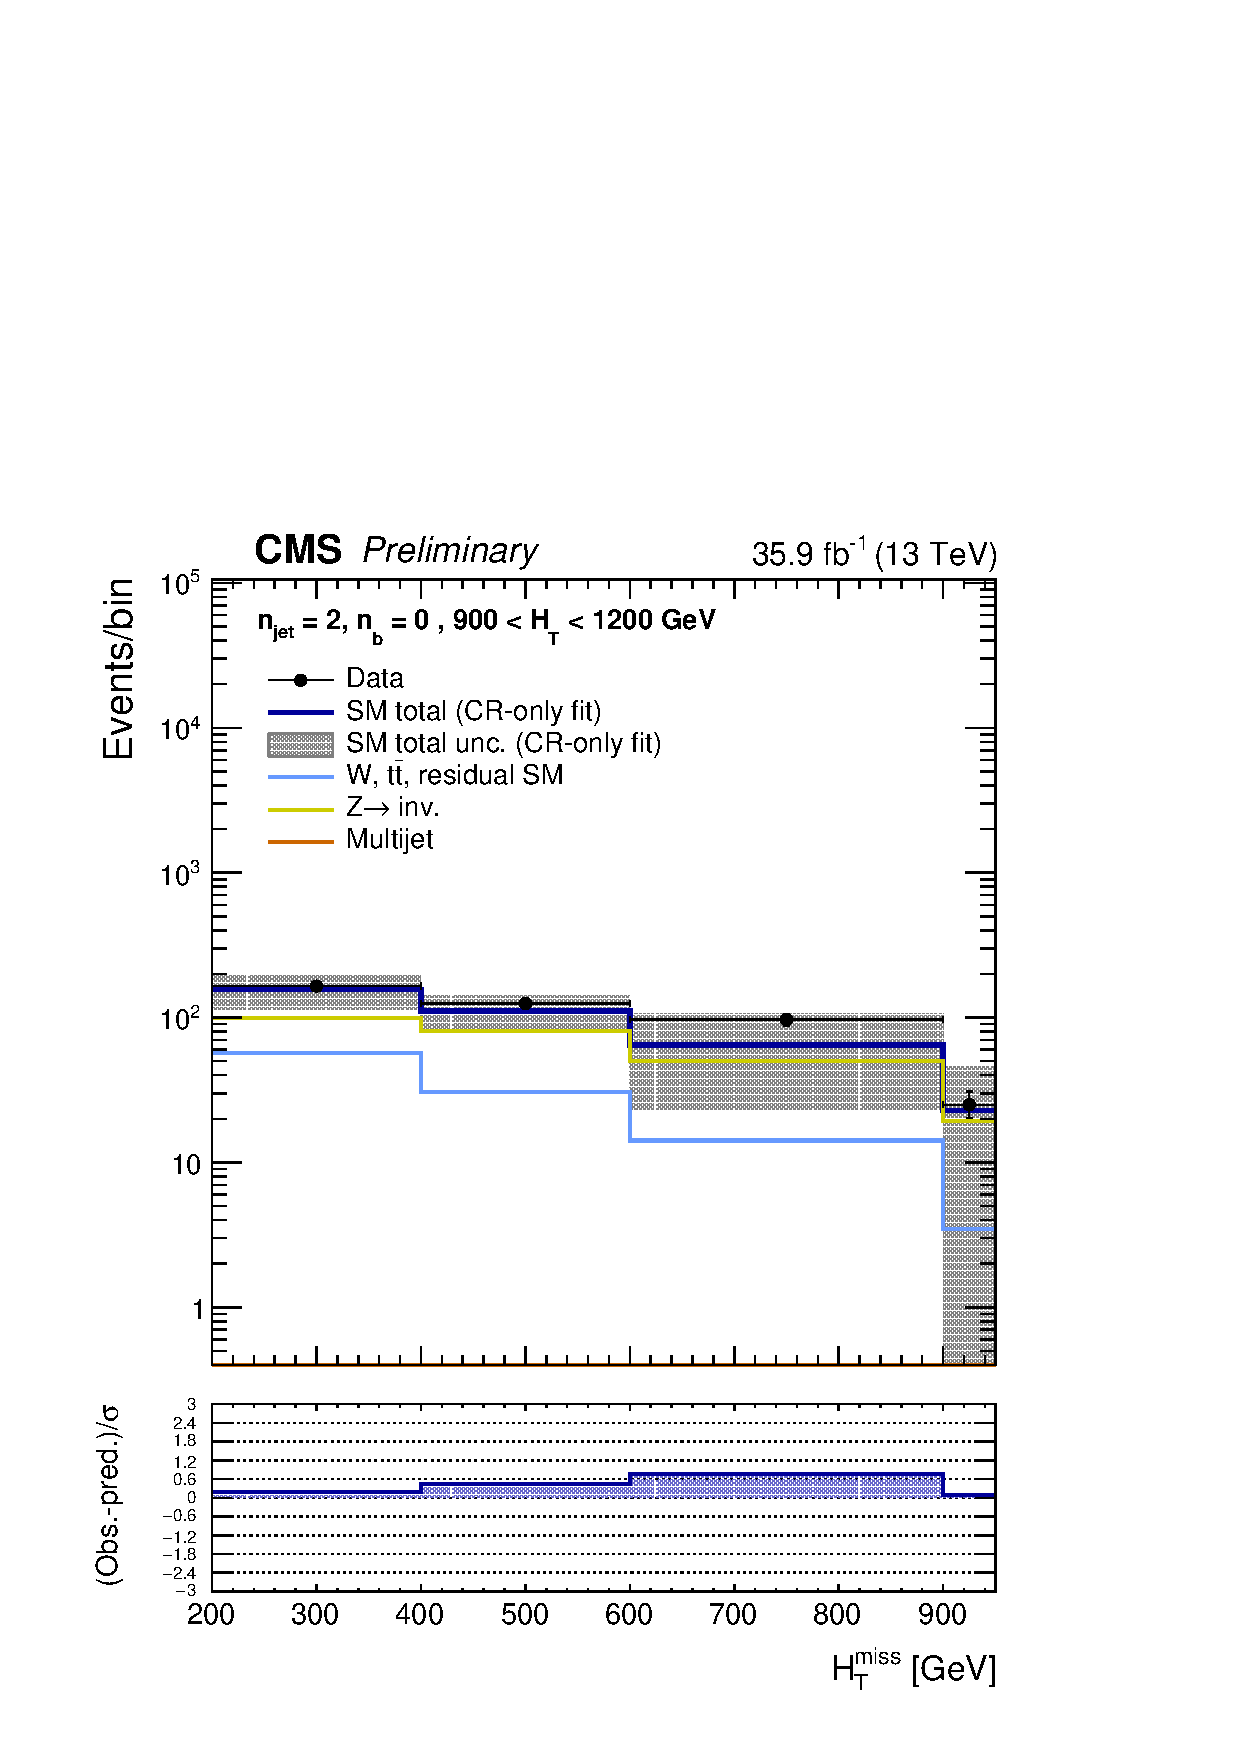
\includegraphics[width=0.49\textwidth]{figures/results/36invfb_preapproval//crfit/shapes//mhtShape_eq0b_eq2j_900_1200_crfit.pdf}}
    \subfigure[$\scalht > 1200\GeV$]{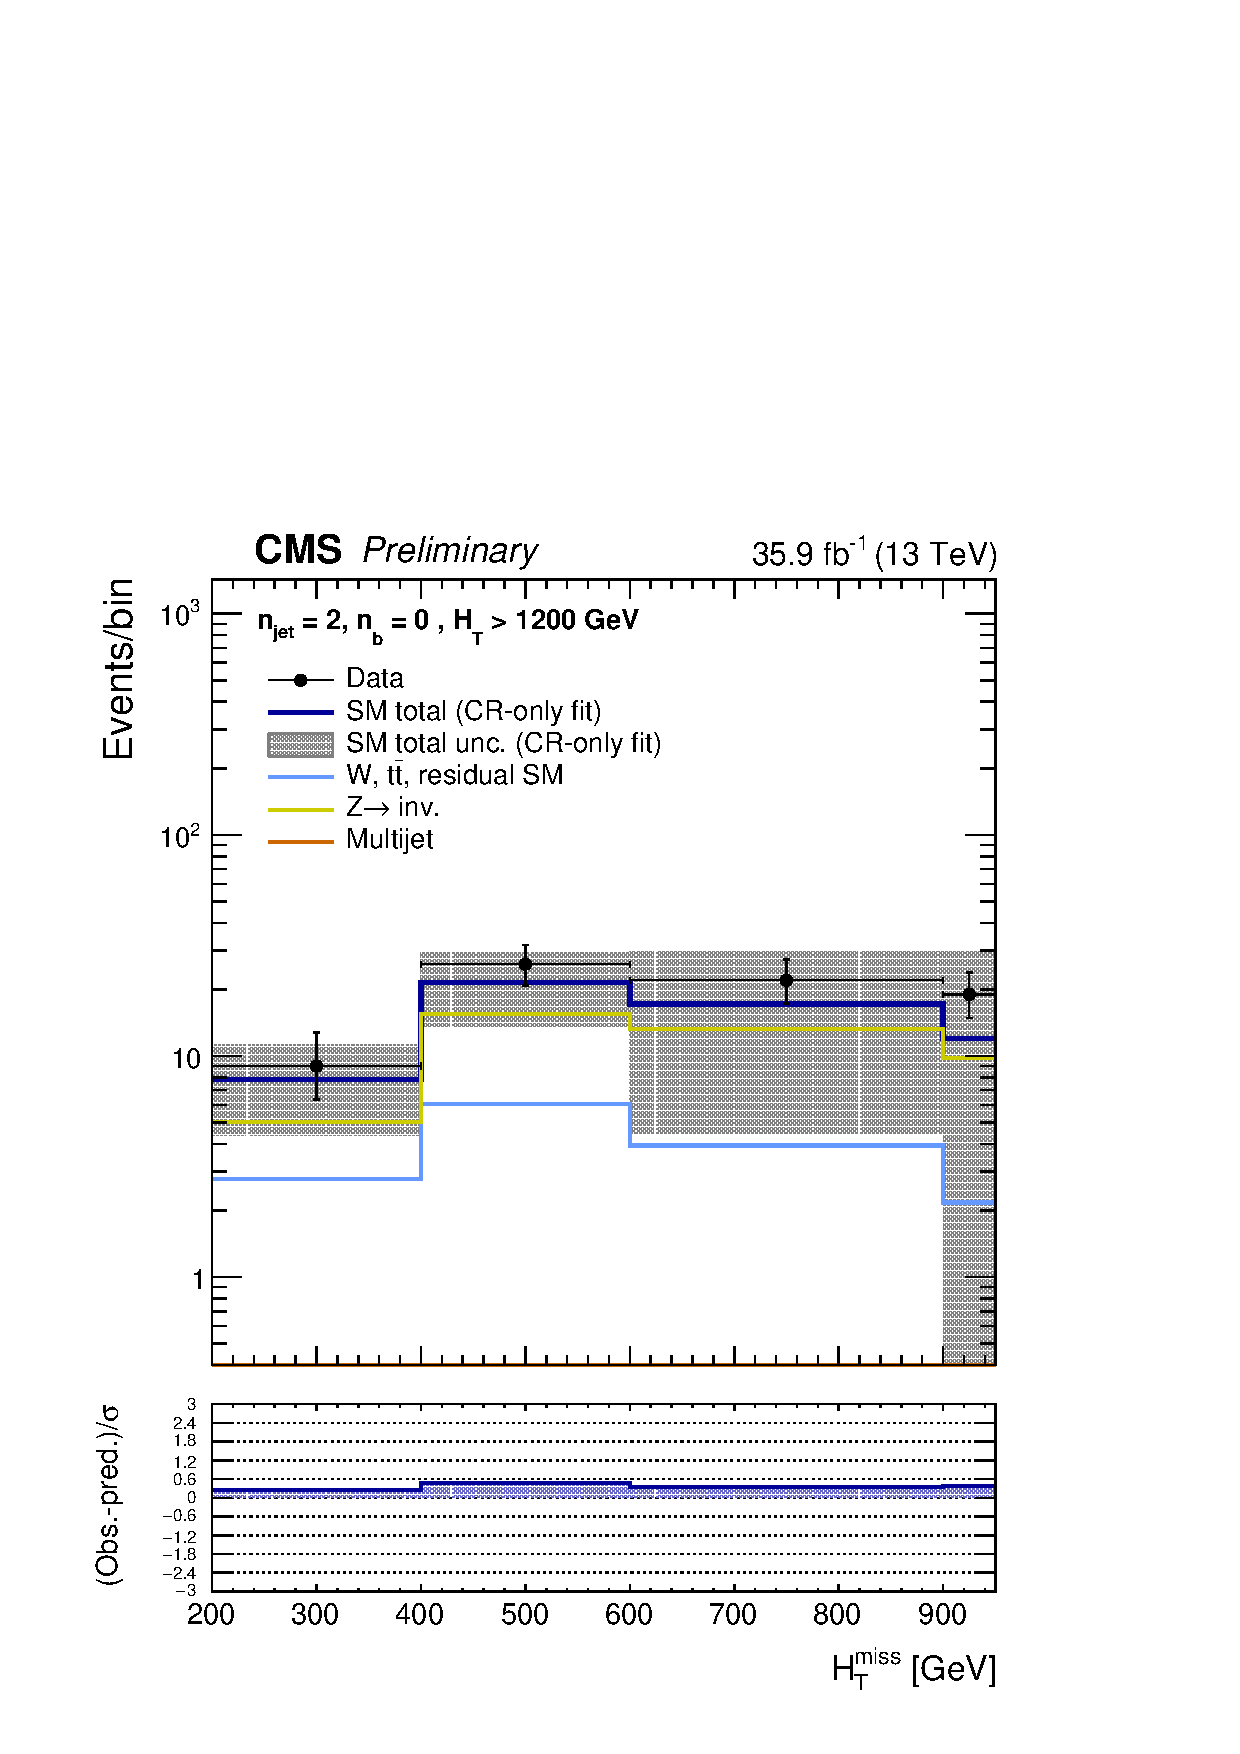
\includegraphics[width=0.49\textwidth]{figures/results/36invfb_preapproval//crfit/shapes//mhtShape_eq0b_eq2j_1200_Inf_crfit.pdf}}\\
    \caption{Event yields observed in data (solid circles) and CR-fit SM expectations with their associated uncertainties (green histogram with shaded band) as a function of \HTmiss based on a sample of events that satisfy $\njet = 2$ and $\nb = 0$, as well as the requirements on \scalht indicated by each sub-figure caption. }
    \label{fig:mhtdim_eq2j_eq0b}
  \end{center}
\end{figure}

\clearpage
\begin{figure}[h!]
  \begin{center}
    \subfigure[$400 < \scalht < 600\GeV$]{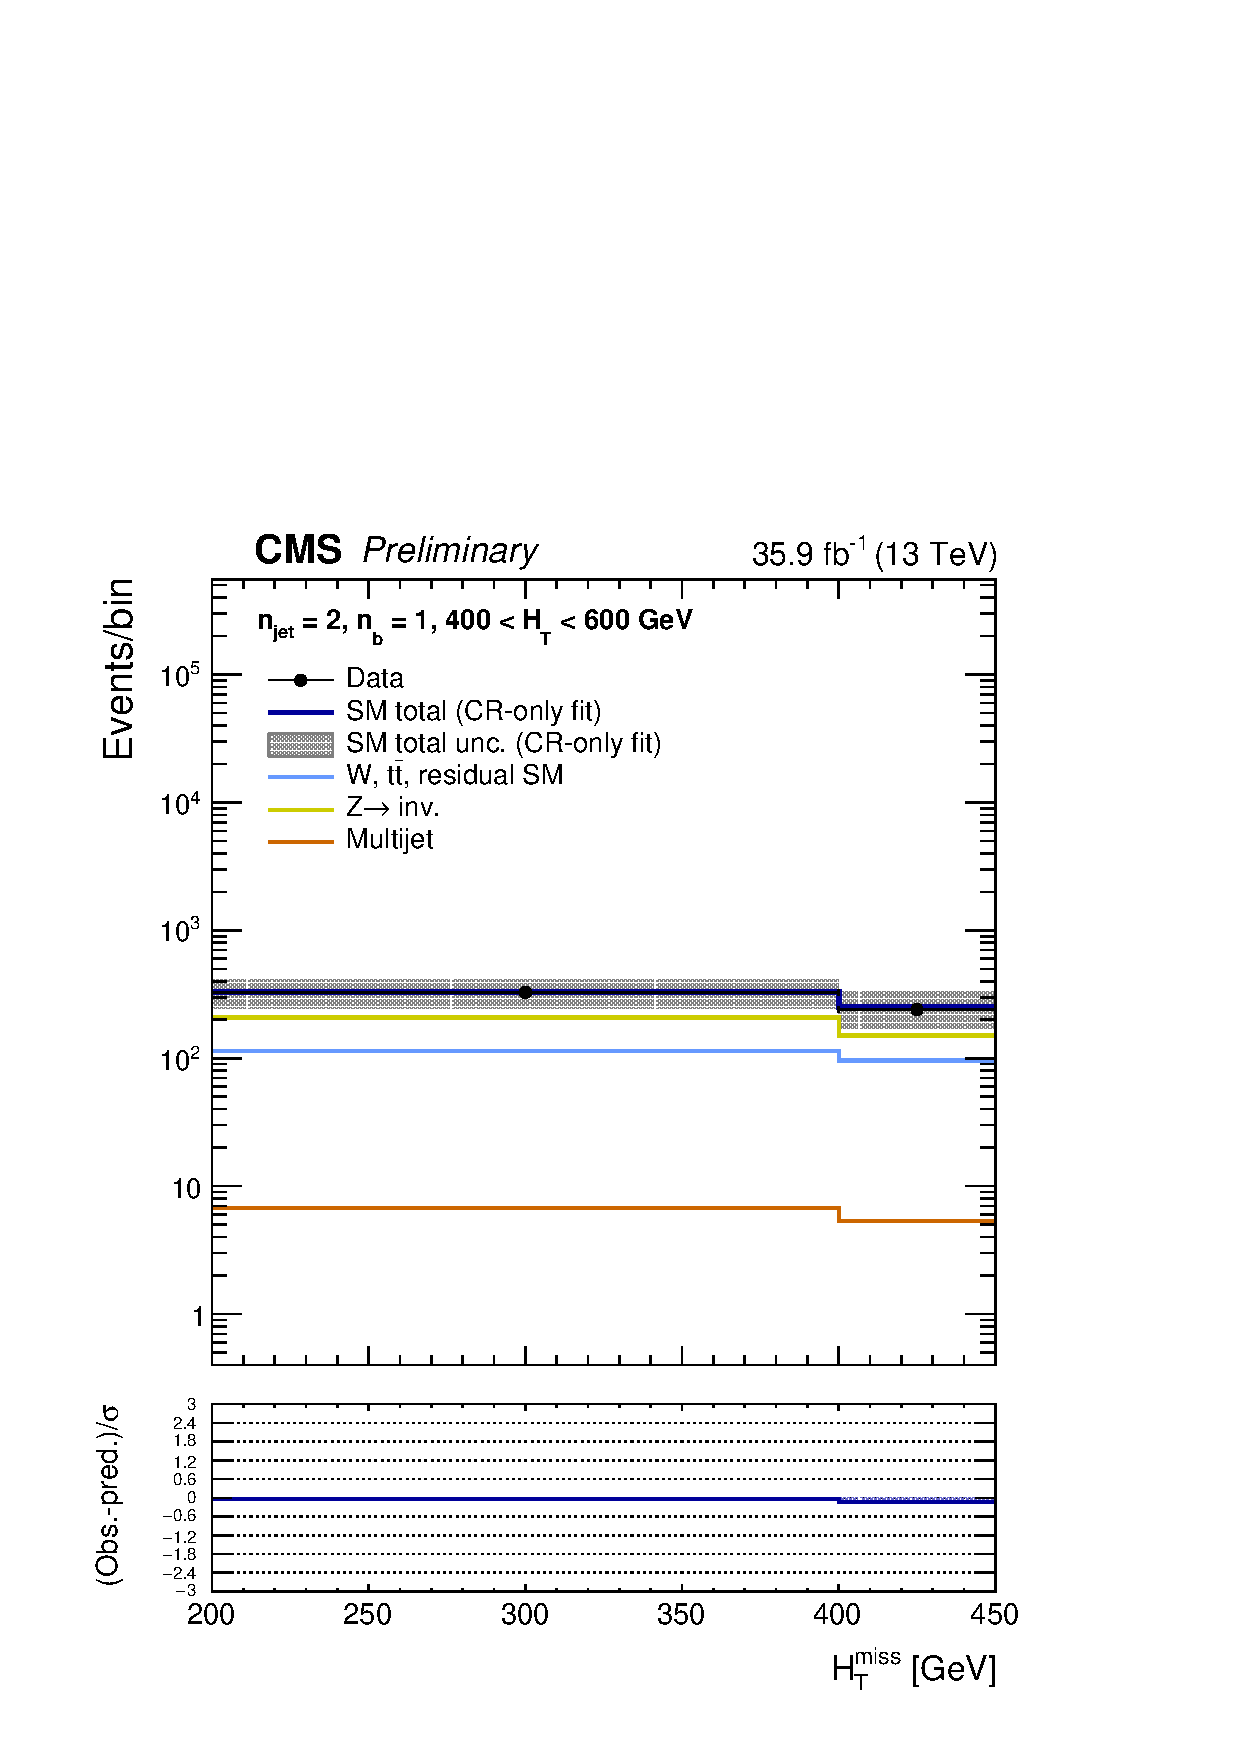
\includegraphics[width=0.49\textwidth]{figures/results/36invfb_preapproval//crfit/shapes//mhtShape_eq1b_eq2j_400_600_crfit.pdf}}
    \subfigure[$600 < \scalht < 900\GeV$]{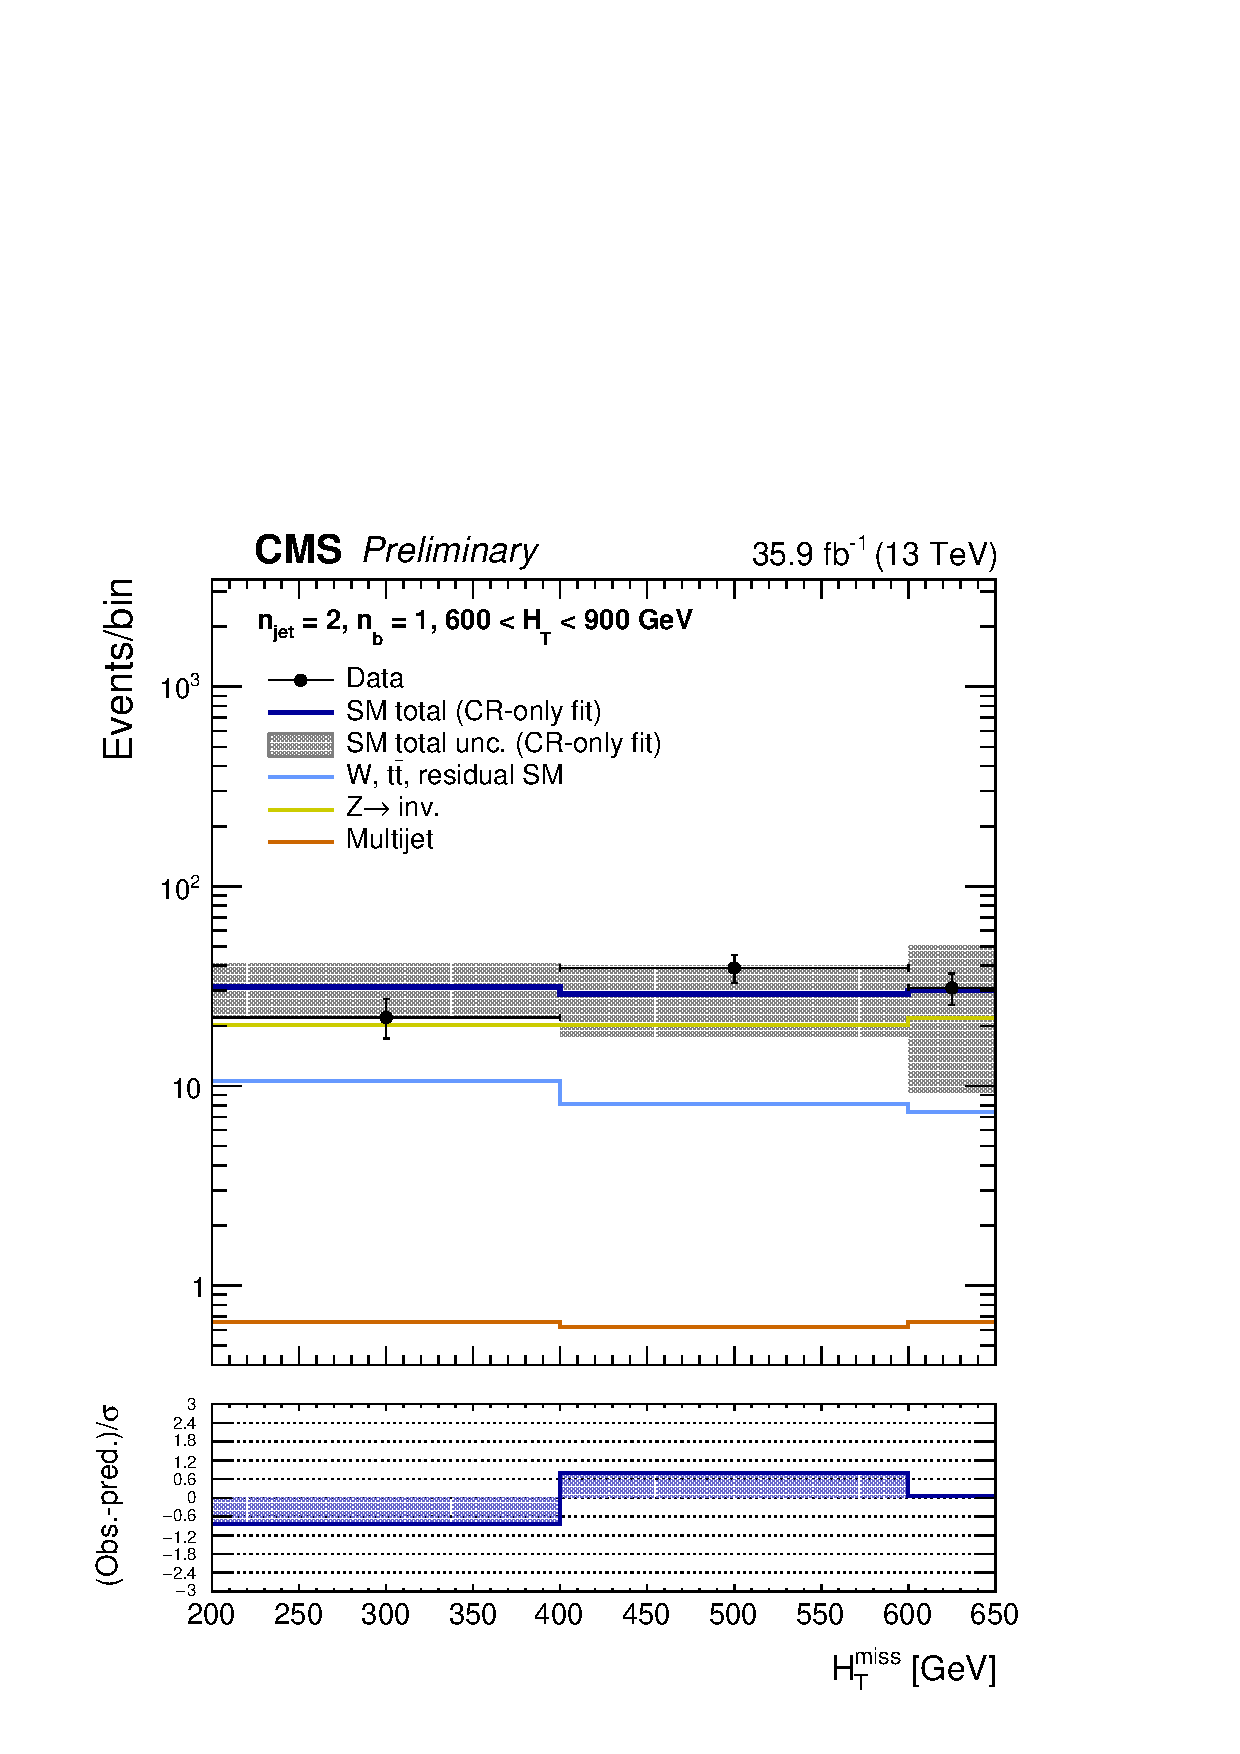
\includegraphics[width=0.49\textwidth]{figures/results/36invfb_preapproval//crfit/shapes//mhtShape_eq1b_eq2j_600_900_crfit.pdf}}\\
    \subfigure[$900 < \scalht < 1200\GeV$]{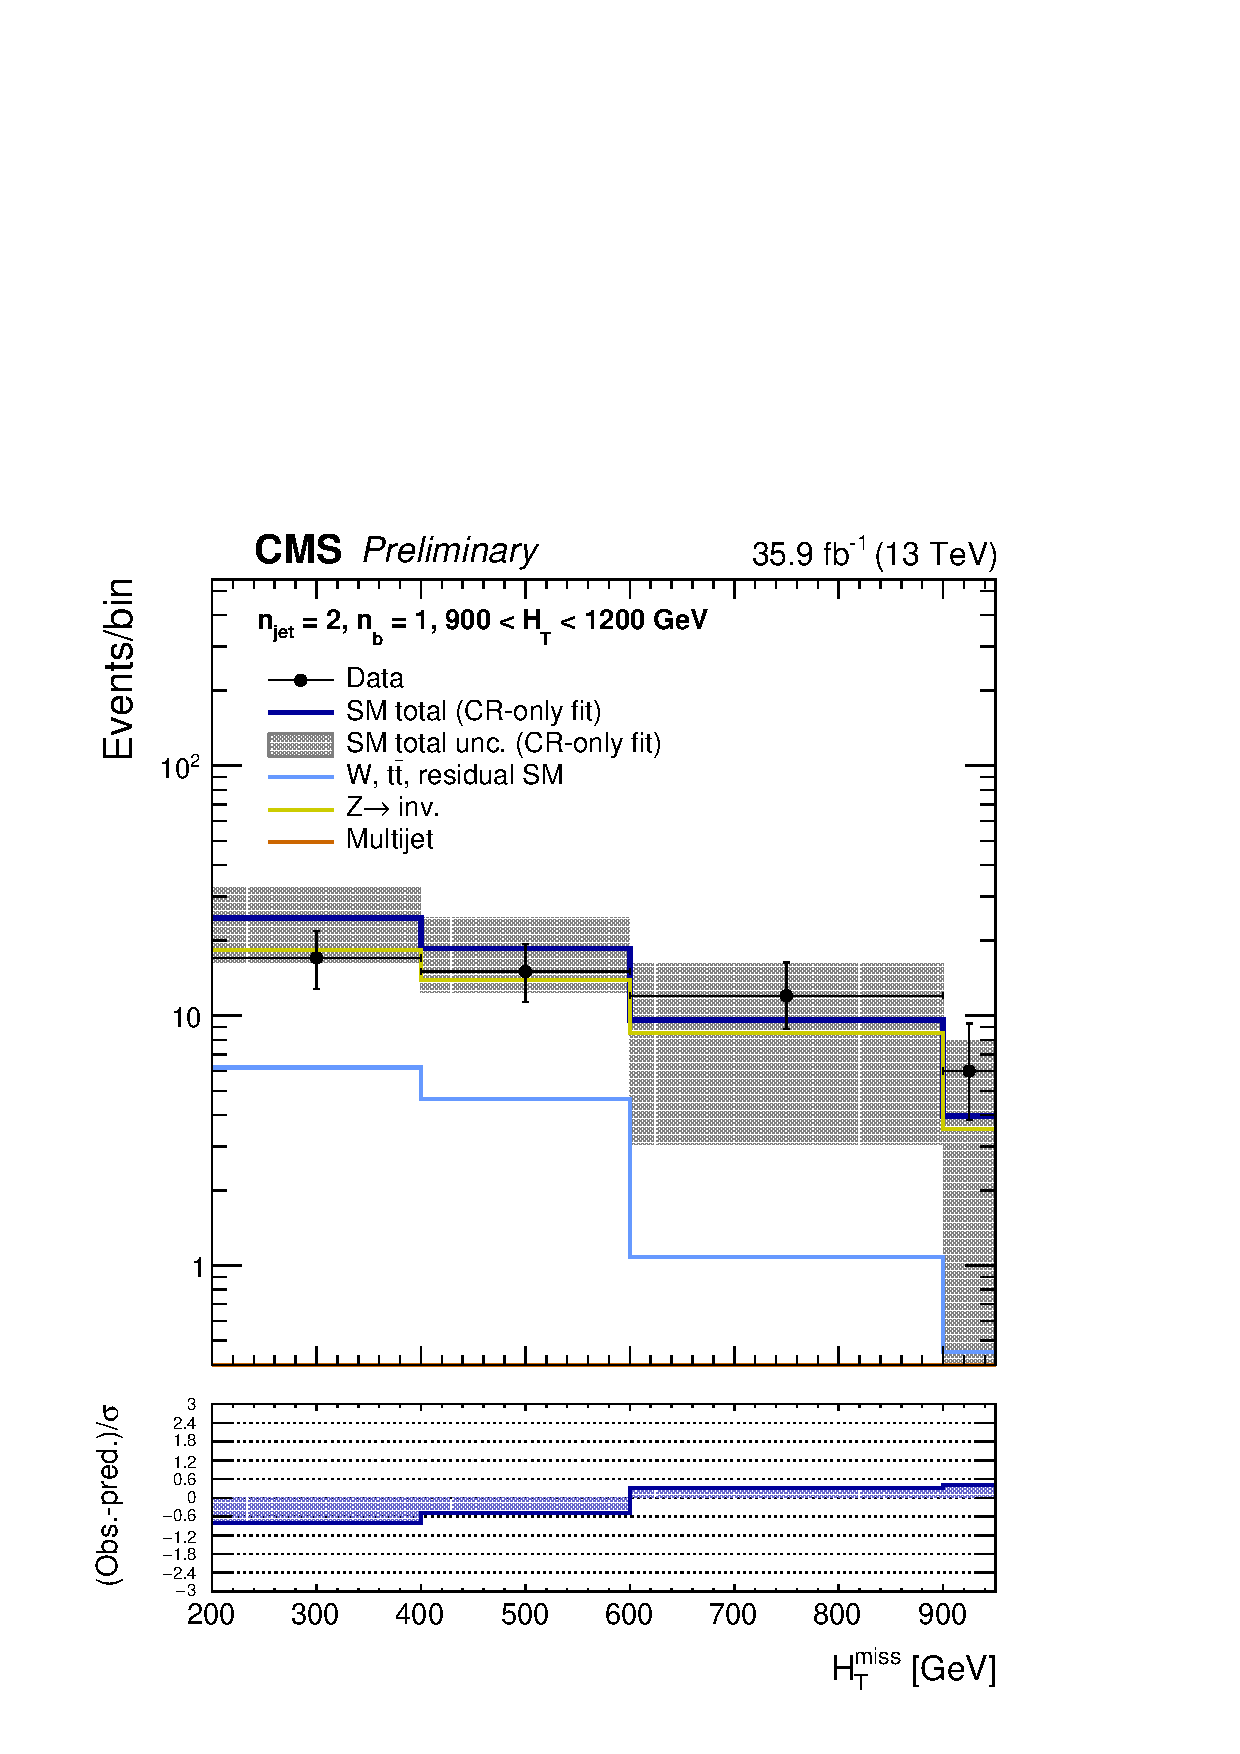
\includegraphics[width=0.49\textwidth]{figures/results/36invfb_preapproval//crfit/shapes//mhtShape_eq1b_eq2j_900_1200_crfit.pdf}}
    \subfigure[$\scalht > 1200\GeV$]{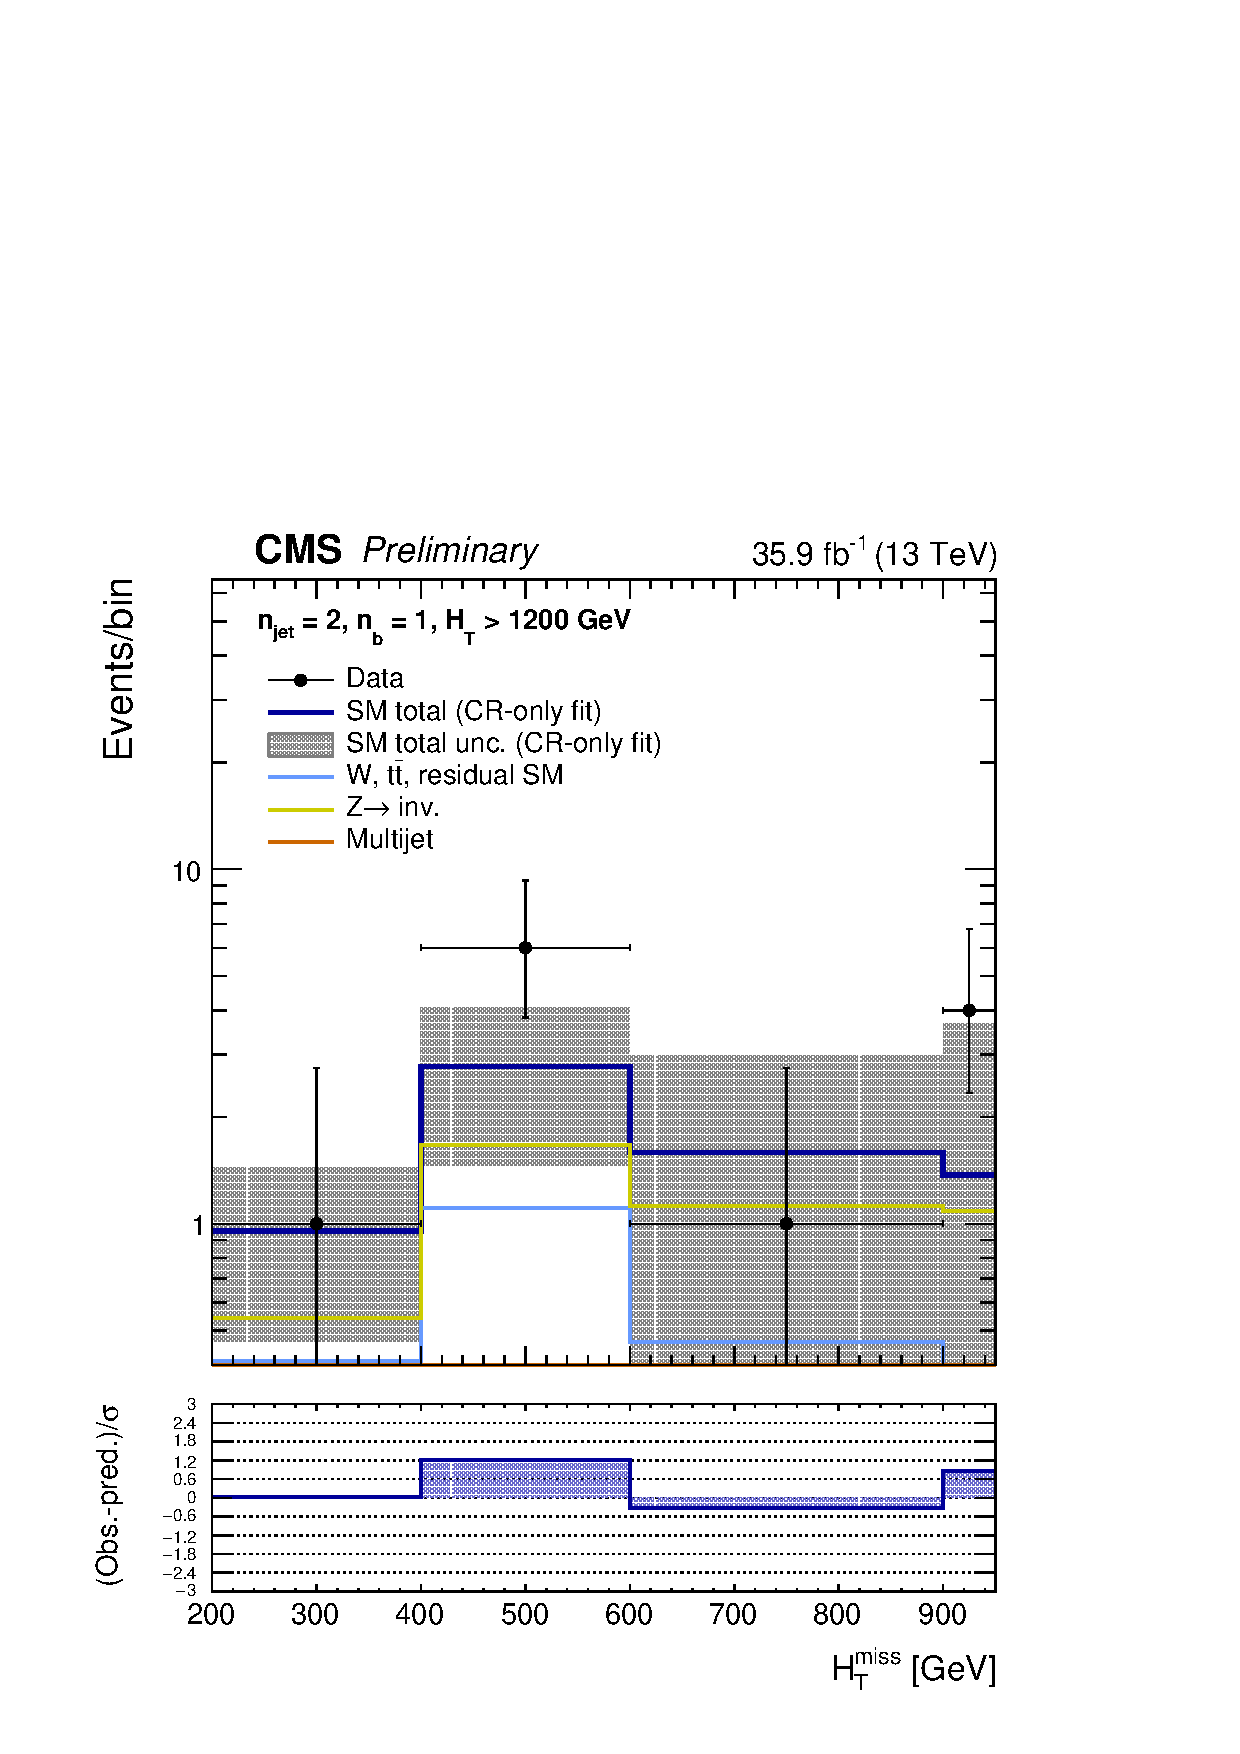
\includegraphics[width=0.49\textwidth]{figures/results/36invfb_preapproval//crfit/shapes//mhtShape_eq1b_eq2j_1200_Inf_crfit.pdf}}\\
    \caption{Event yields observed in data (solid circles) and CR-fit SM expectations with their associated uncertainties (green histogram with shaded band) as a function of \HTmiss based on a sample of events that satisfy $\njet = 2$ and $\nb = 1$, as well as the requirements on \scalht indicated by each sub-figure caption. }
    \label{fig:mhtdim_eq2j_eq1b}
  \end{center}
\end{figure}

\clearpage
\begin{figure}[h!]
  \begin{center}
    \subfigure[$400 < \scalht < 600\GeV$]{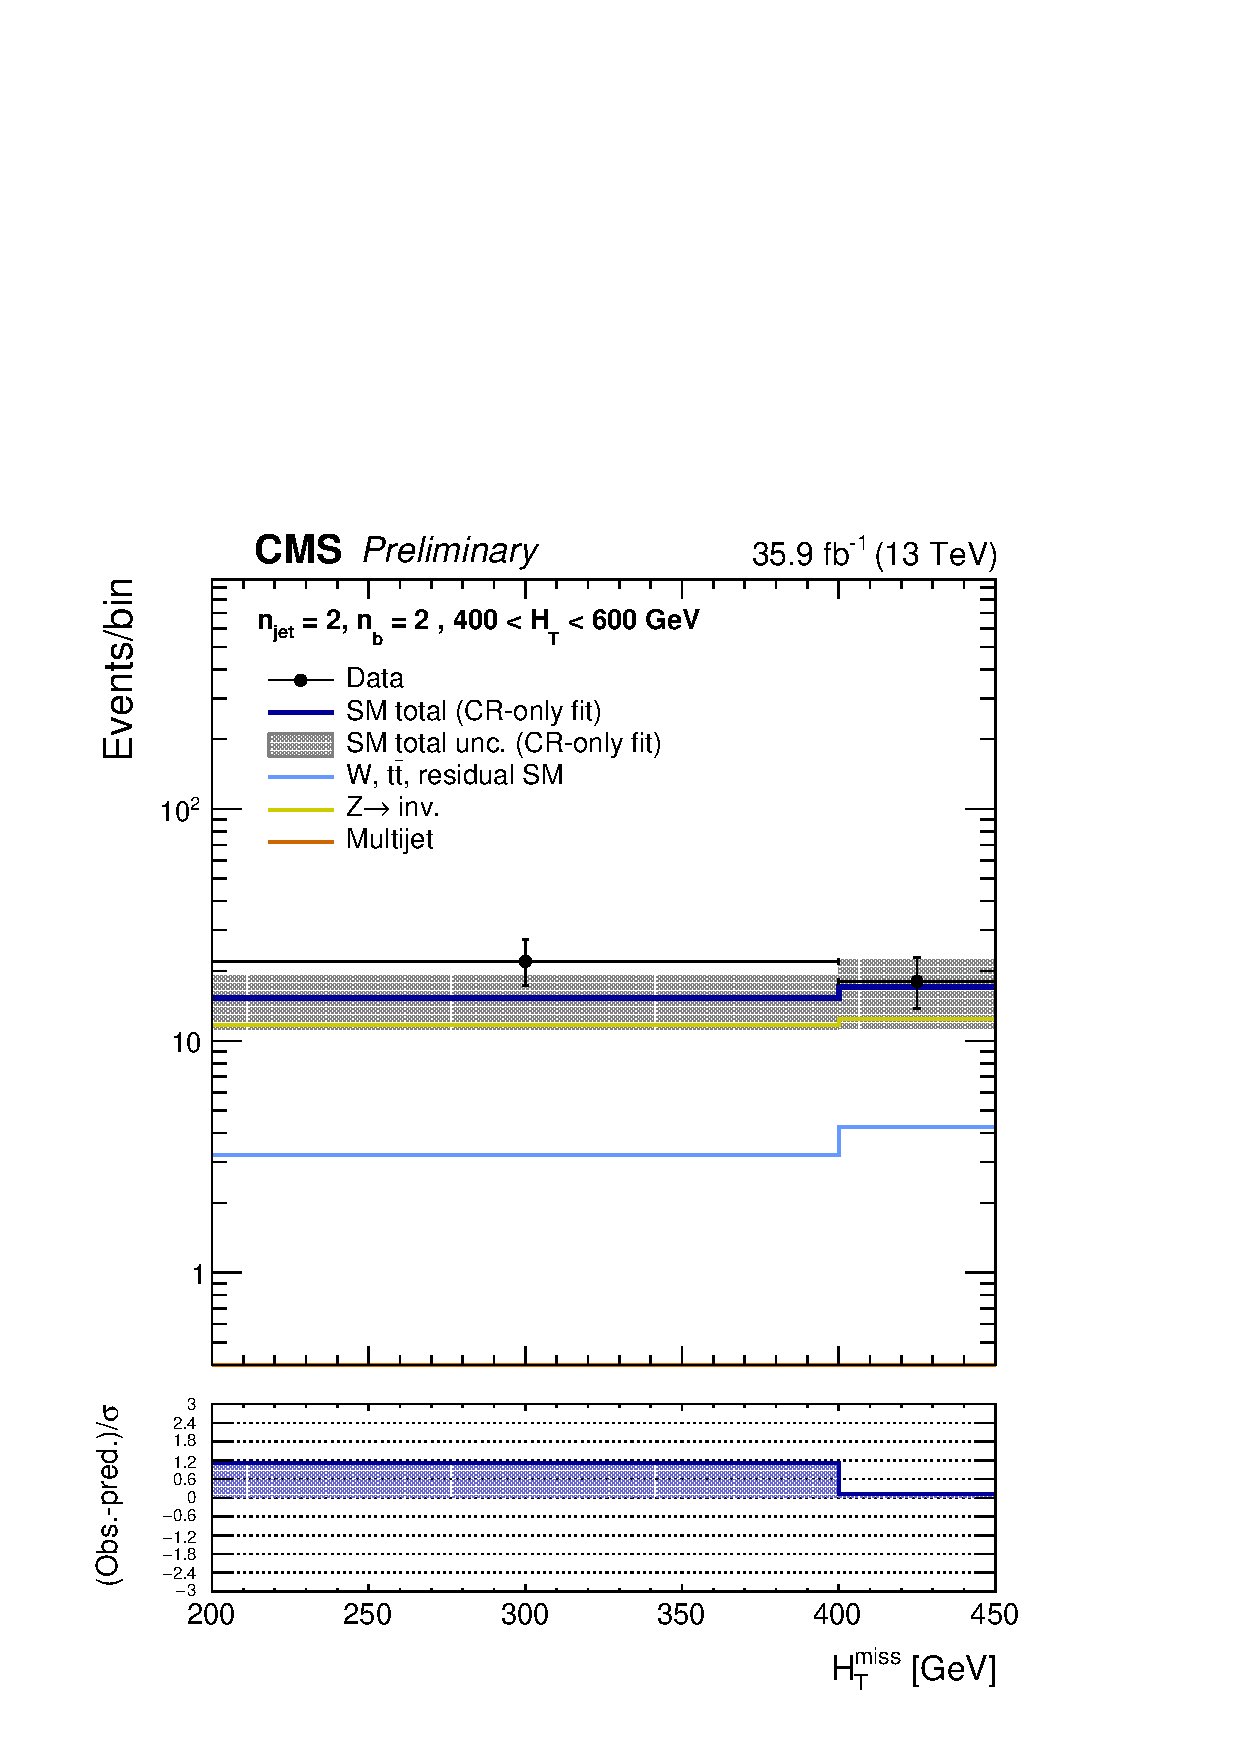
\includegraphics[width=0.49\textwidth]{figures/results/36invfb_preapproval//crfit/shapes//mhtShape_eq2b_eq2j_400_600_crfit.pdf}}
    \caption{Event yields observed in data (solid circles) and CR-fit SM expectations with their associated uncertainties (green histogram with shaded band) as a function of \HTmiss based on a sample of events that satisfy $\njet = 2$ and $\nb = 2$, as well as the requirements on \scalht indicated by each sub-figure caption. }
    \label{fig:mhtdim_eq2j_eq2b}
  \end{center}
\end{figure}

\clearpage
\begin{figure}[h!]
  \begin{center}
    \subfigure[$400 < \scalht < 600\GeV$]{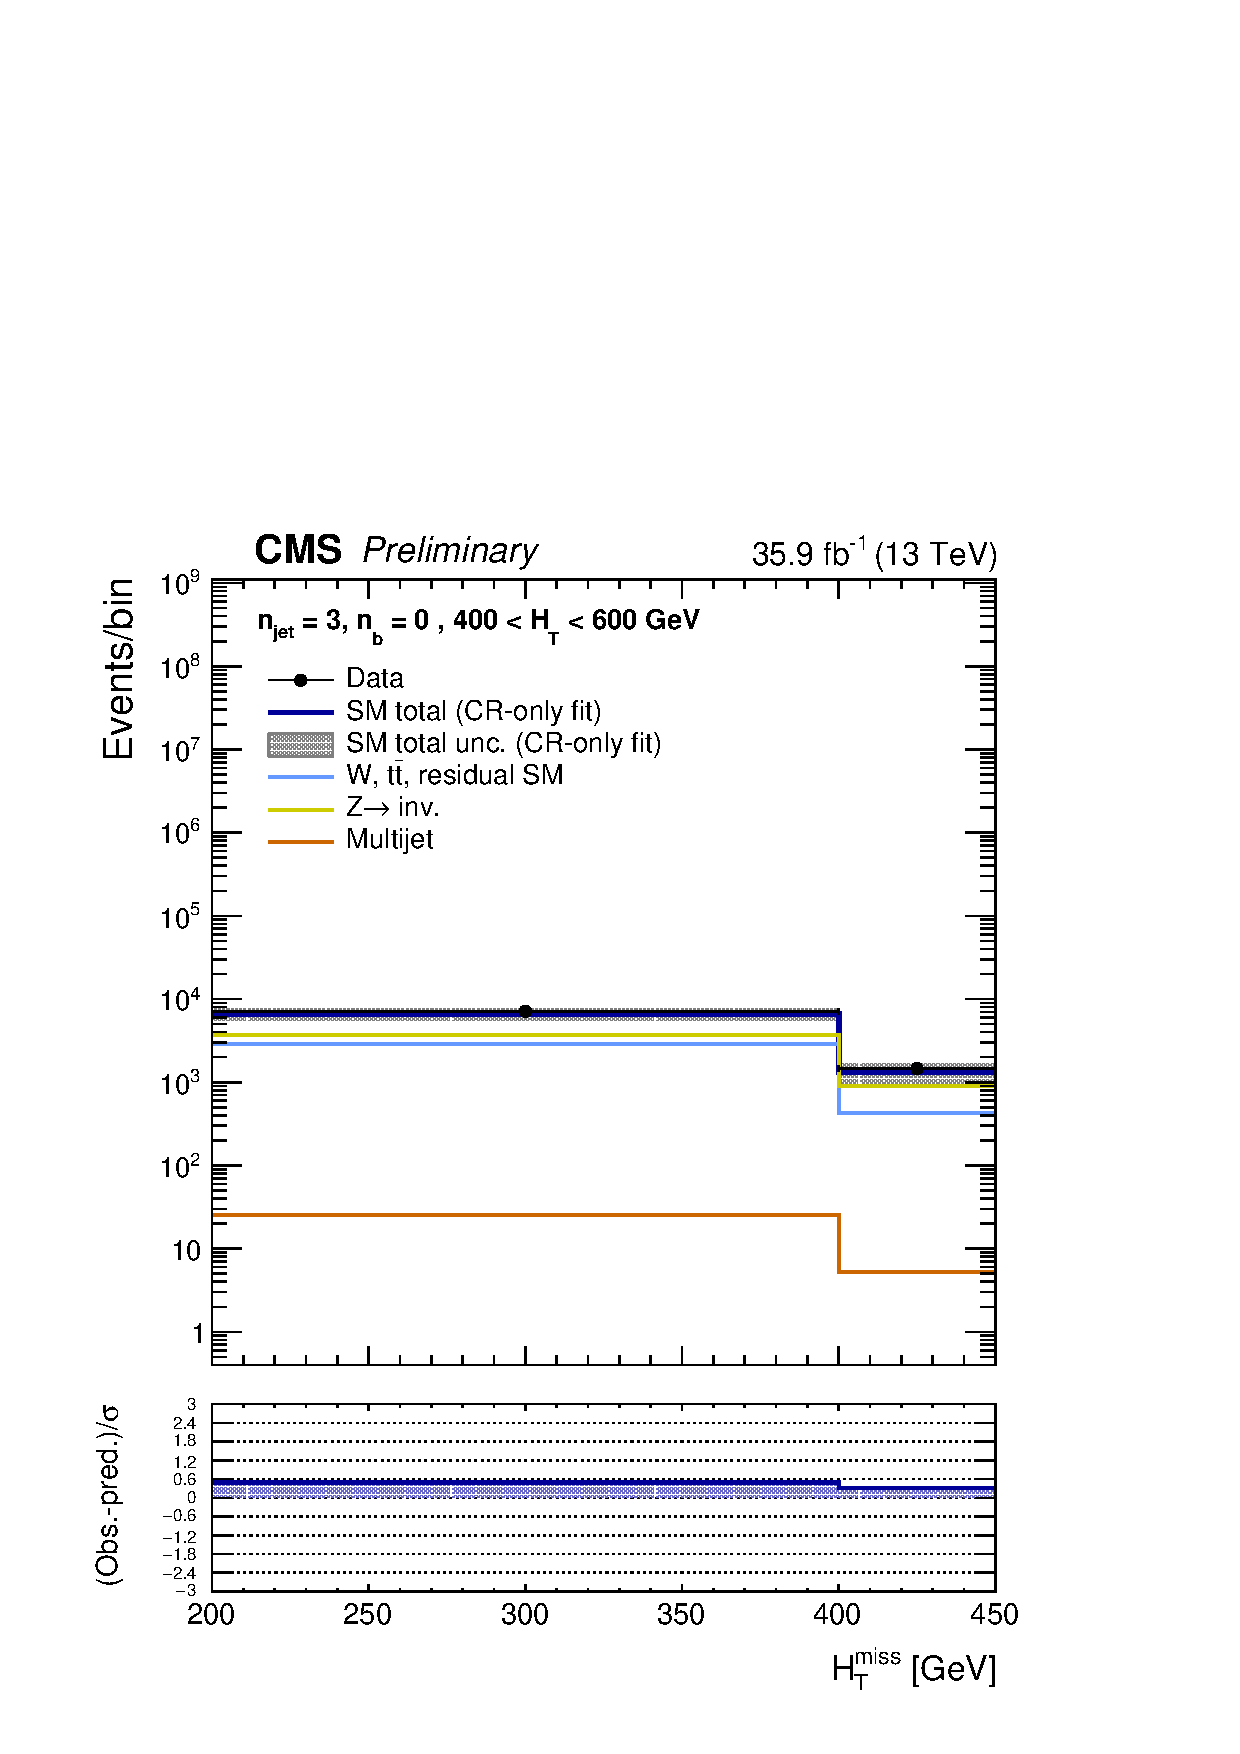
\includegraphics[width=0.49\textwidth]{figures/results/36invfb_preapproval//crfit/shapes//mhtShape_eq0b_eq3j_400_600_crfit.pdf}}
    \subfigure[$600 < \scalht < 900\GeV$]{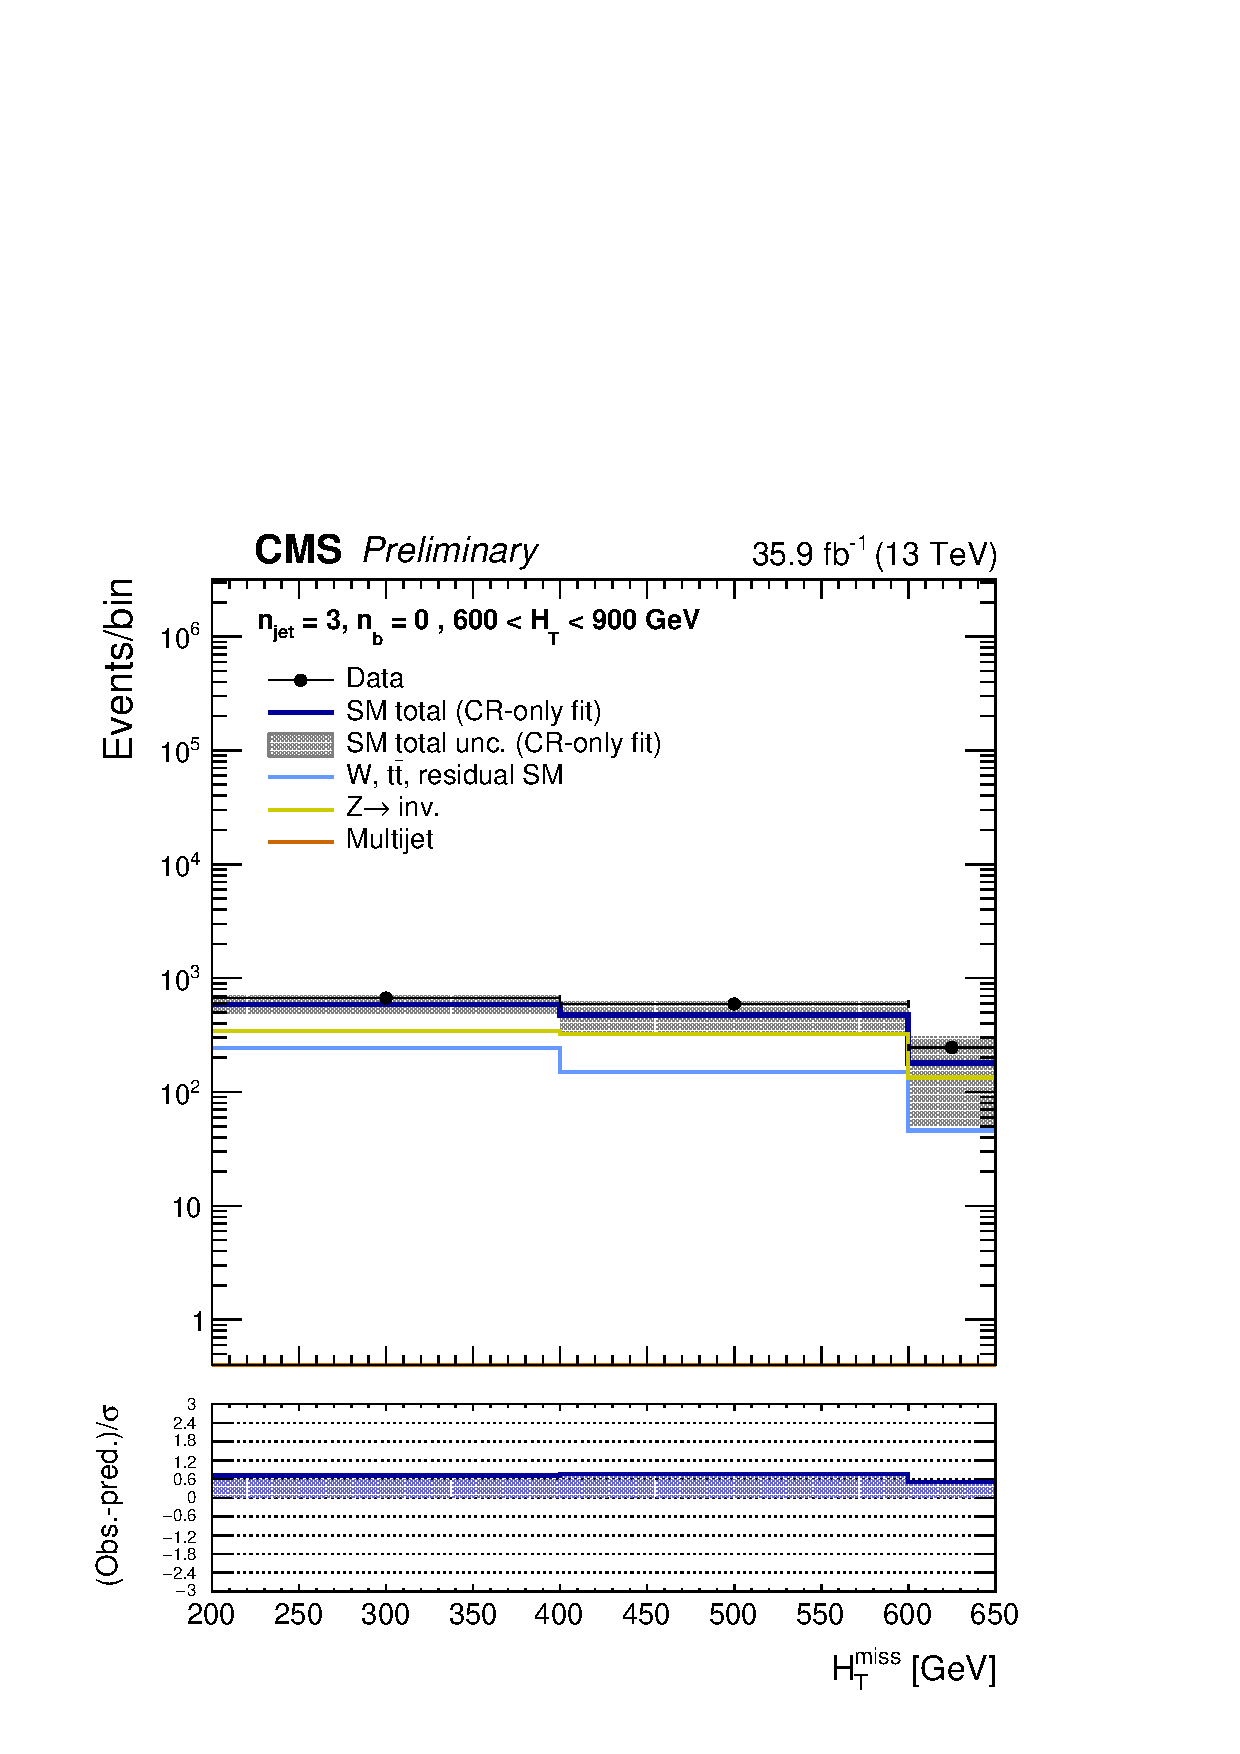
\includegraphics[width=0.49\textwidth]{figures/results/36invfb_preapproval//crfit/shapes//mhtShape_eq0b_eq3j_600_900_crfit.pdf}}\\
    \subfigure[$900 < \scalht < 1200\GeV$]{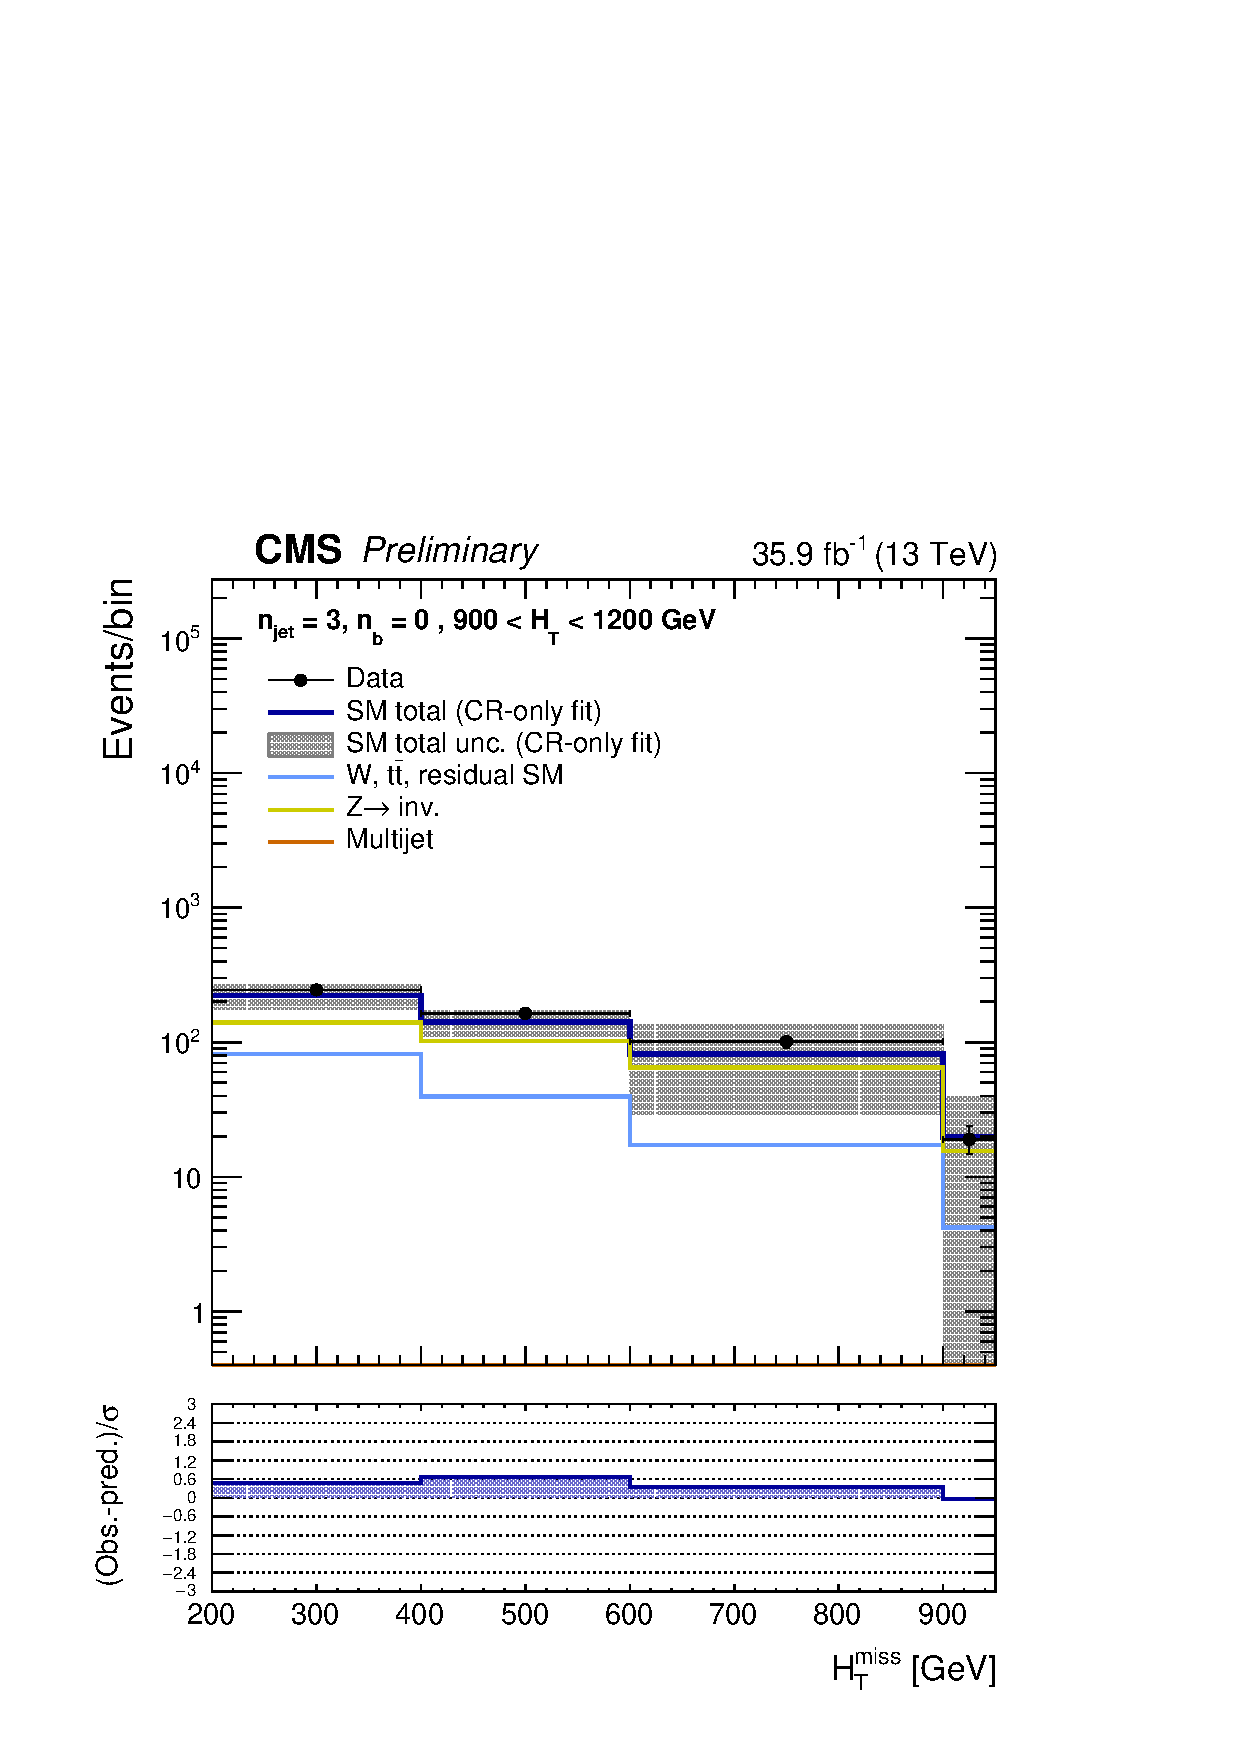
\includegraphics[width=0.49\textwidth]{figures/results/36invfb_preapproval//crfit/shapes//mhtShape_eq0b_eq3j_900_1200_crfit.pdf}}
    \subfigure[$\scalht > 1200\GeV$]{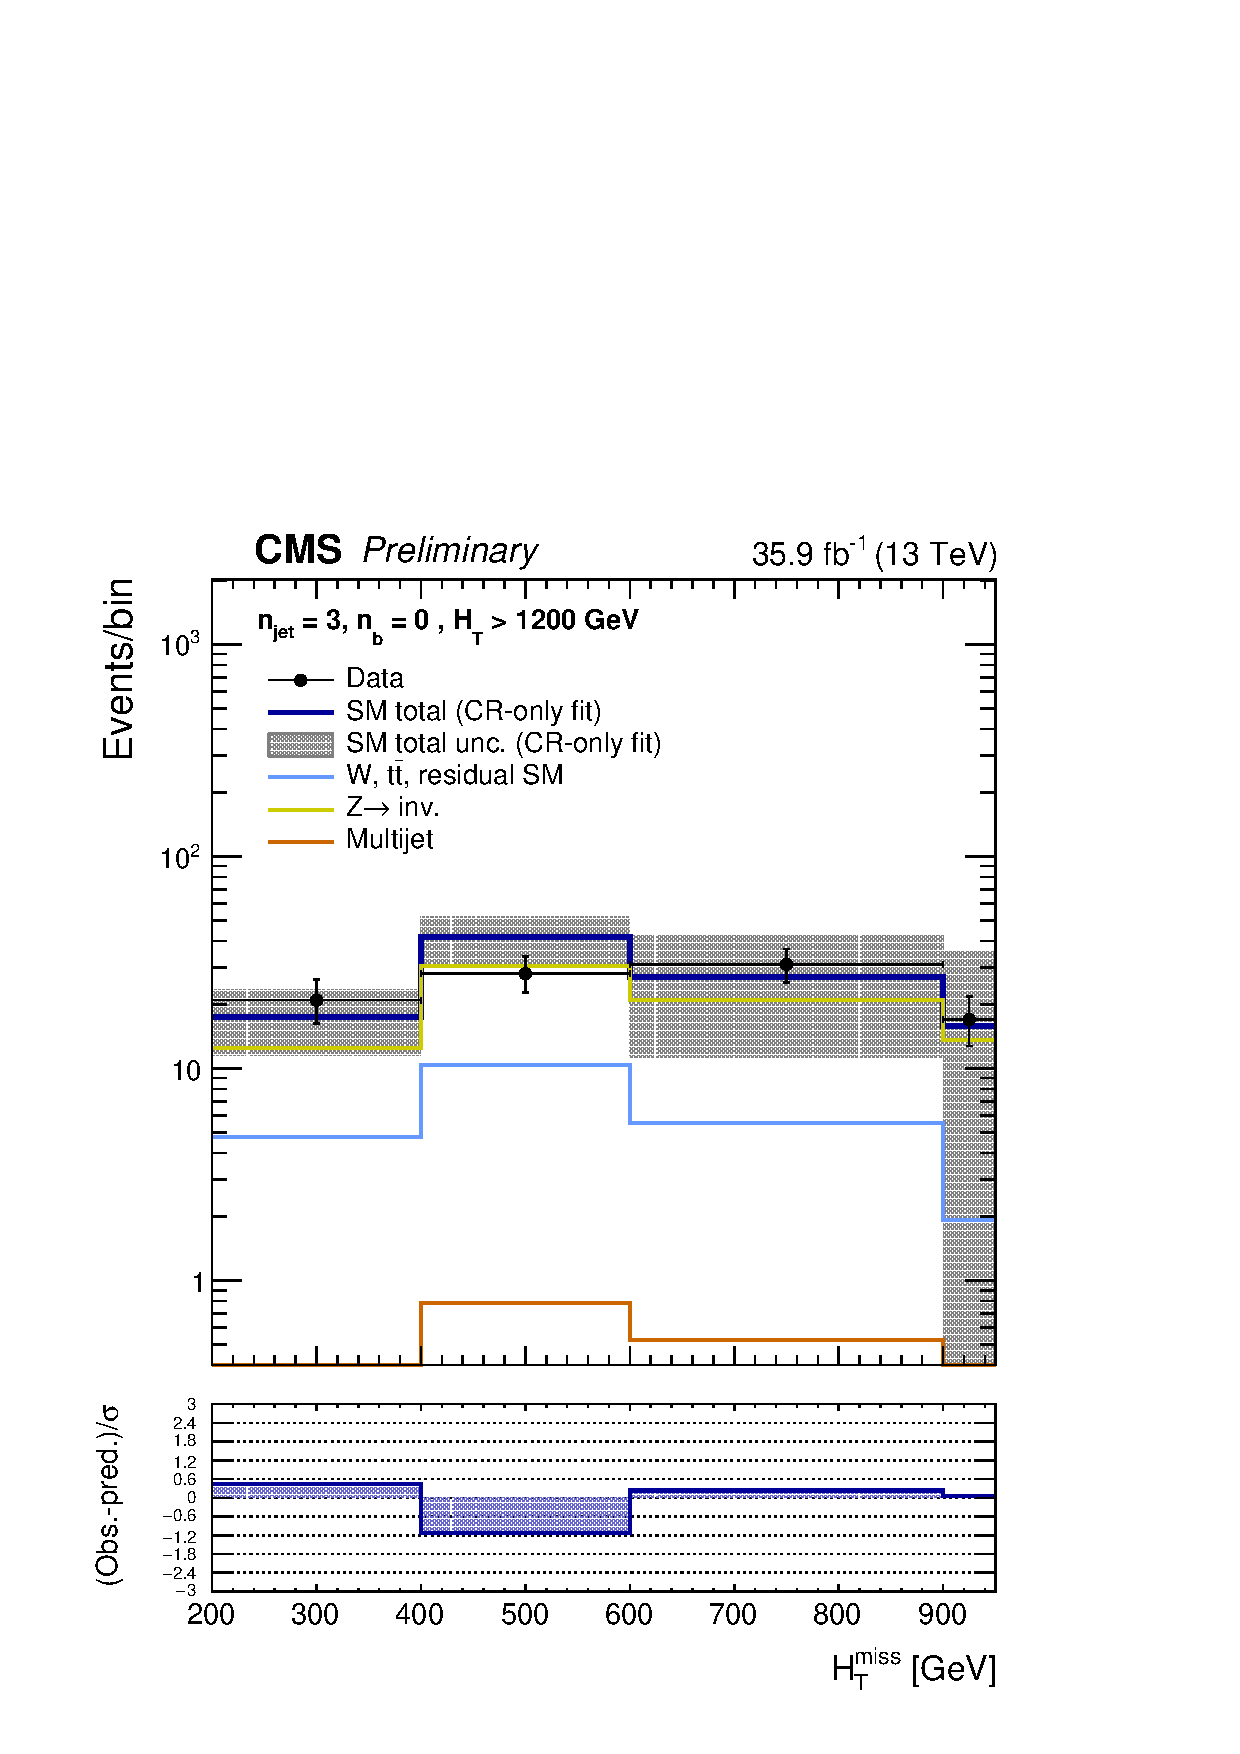
\includegraphics[width=0.49\textwidth]{figures/results/36invfb_preapproval//crfit/shapes//mhtShape_eq0b_eq3j_1200_Inf_crfit.pdf}}\\
    \caption{Event yields observed in data (solid circles) and CR-fit SM expectations with their associated uncertainties (green histogram with shaded band) as a function of \HTmiss based on a sample of events that satisfy $\njet = 3$ and $\nb = 0$, as well as the requirements on \scalht indicated by each sub-figure caption. }
    \label{fig:mhtdim_eq3j_eq0b}
  \end{center}
\end{figure}

\clearpage
\begin{figure}[h!]
  \begin{center}
    \subfigure[$400 < \scalht < 600\GeV$]{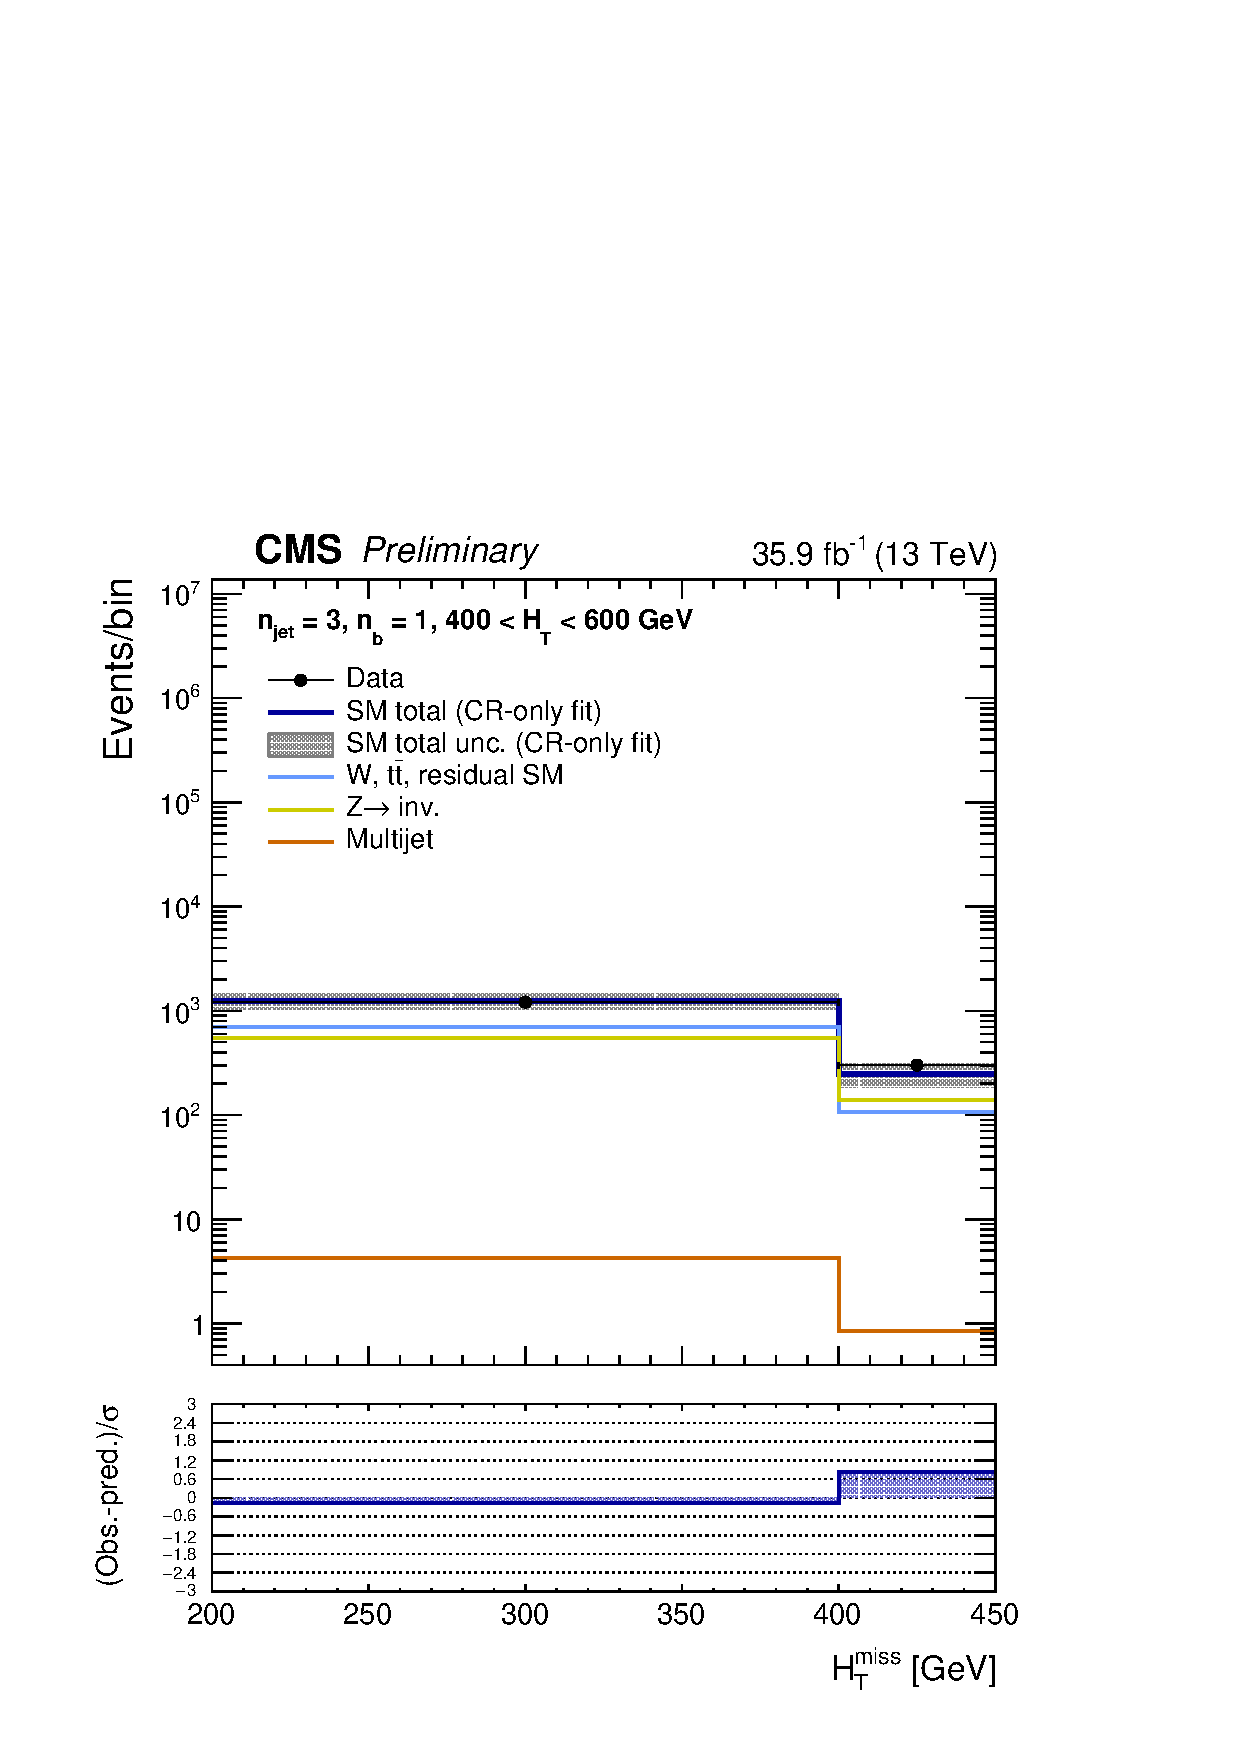
\includegraphics[width=0.49\textwidth]{figures/results/36invfb_preapproval//crfit/shapes//mhtShape_eq1b_eq3j_400_600_crfit.pdf}}
    \subfigure[$600 < \scalht < 900\GeV$]{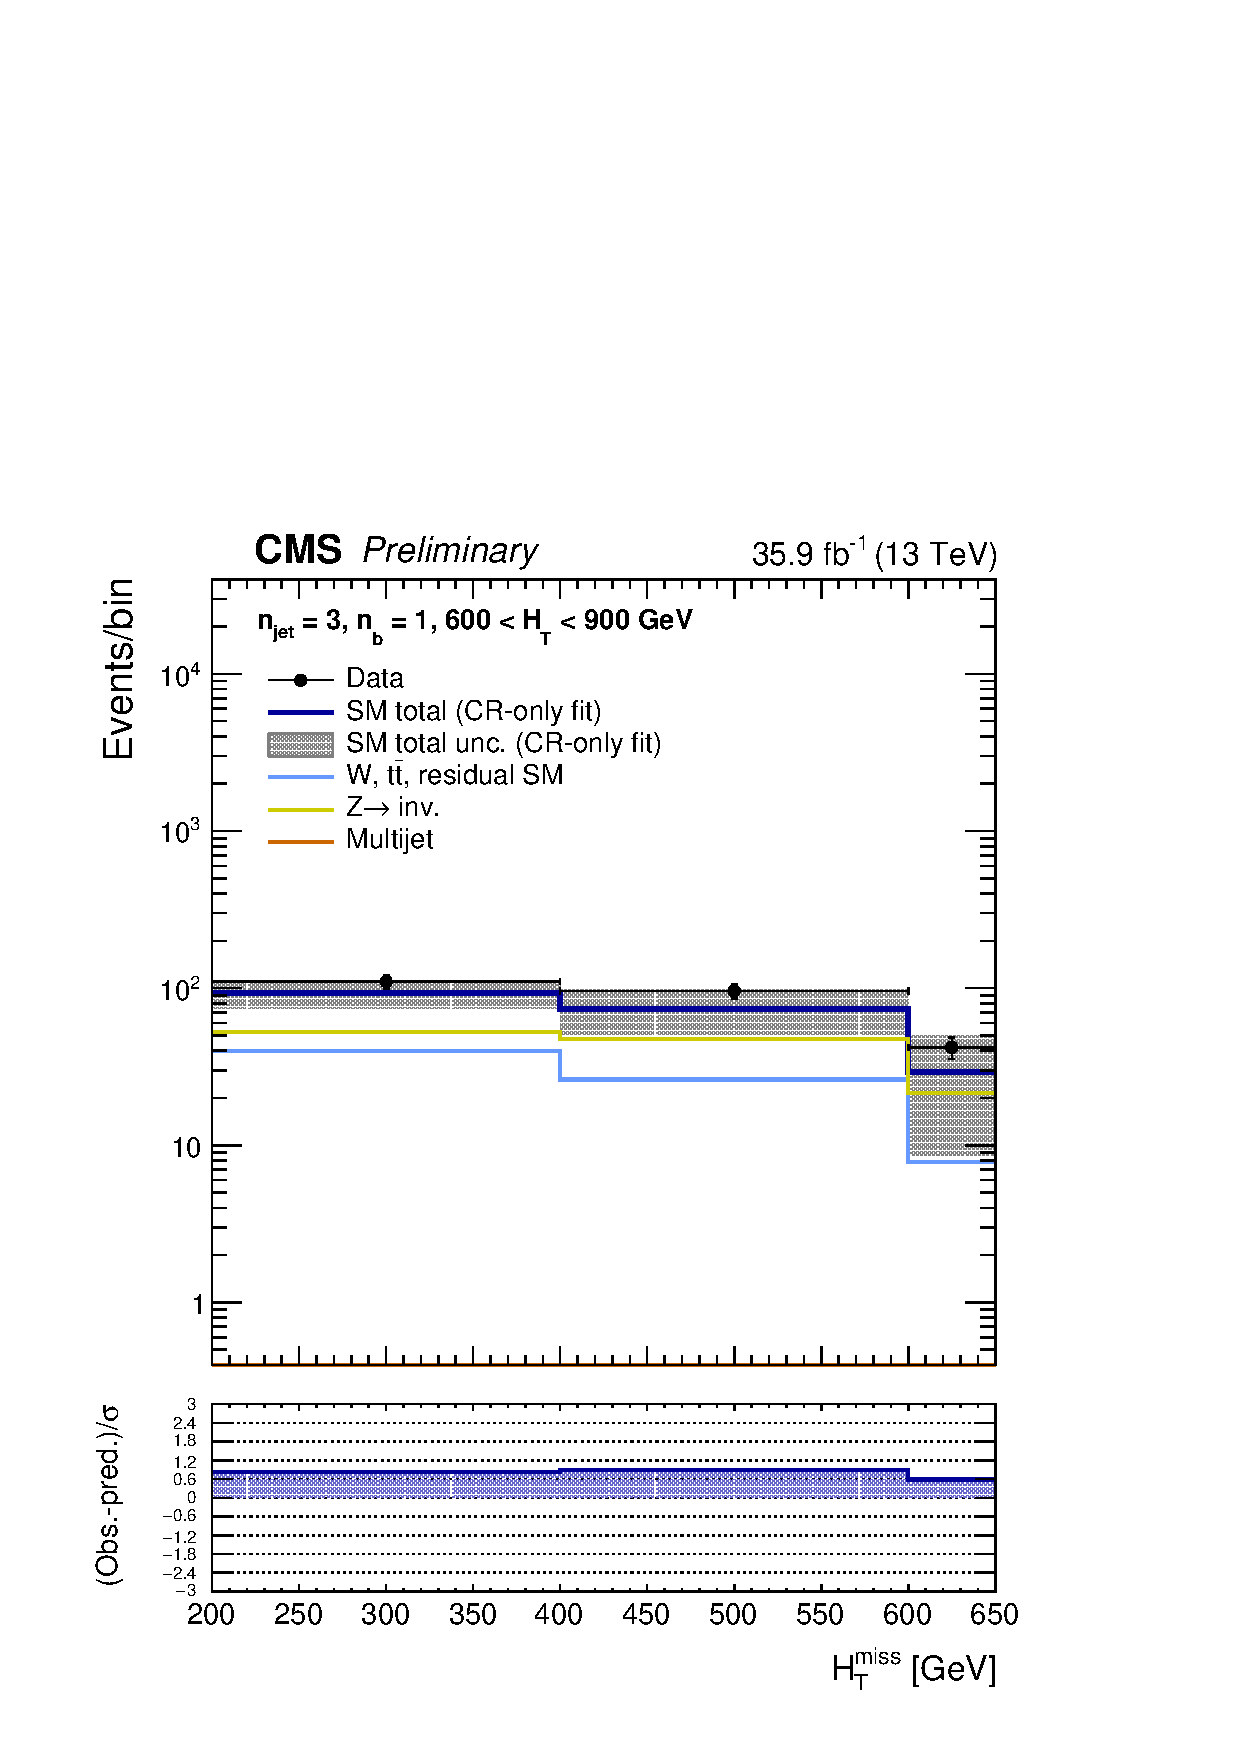
\includegraphics[width=0.49\textwidth]{figures/results/36invfb_preapproval//crfit/shapes//mhtShape_eq1b_eq3j_600_900_crfit.pdf}}\\
    \subfigure[$900 < \scalht < 1200\GeV$]{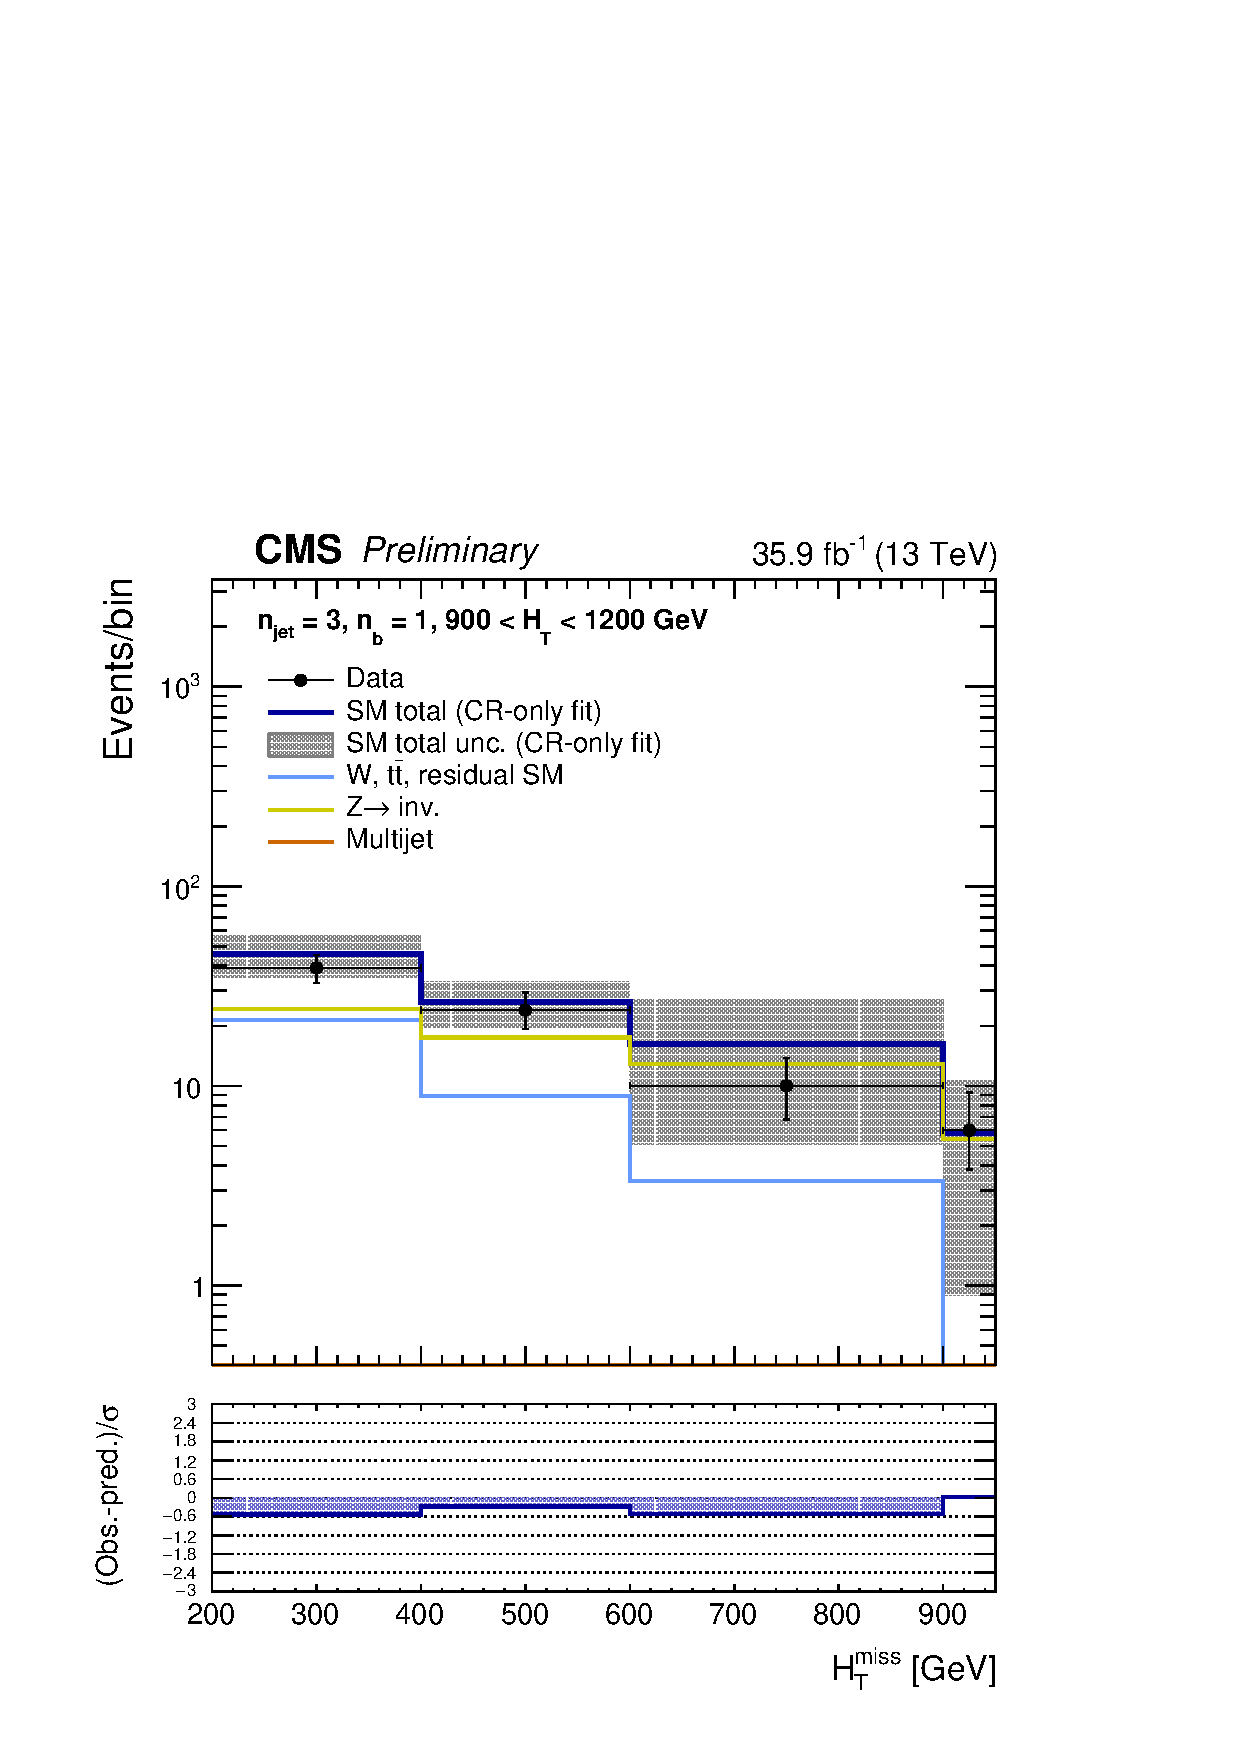
\includegraphics[width=0.49\textwidth]{figures/results/36invfb_preapproval//crfit/shapes//mhtShape_eq1b_eq3j_900_1200_crfit.pdf}}
    \subfigure[$\scalht > 1200\GeV$]{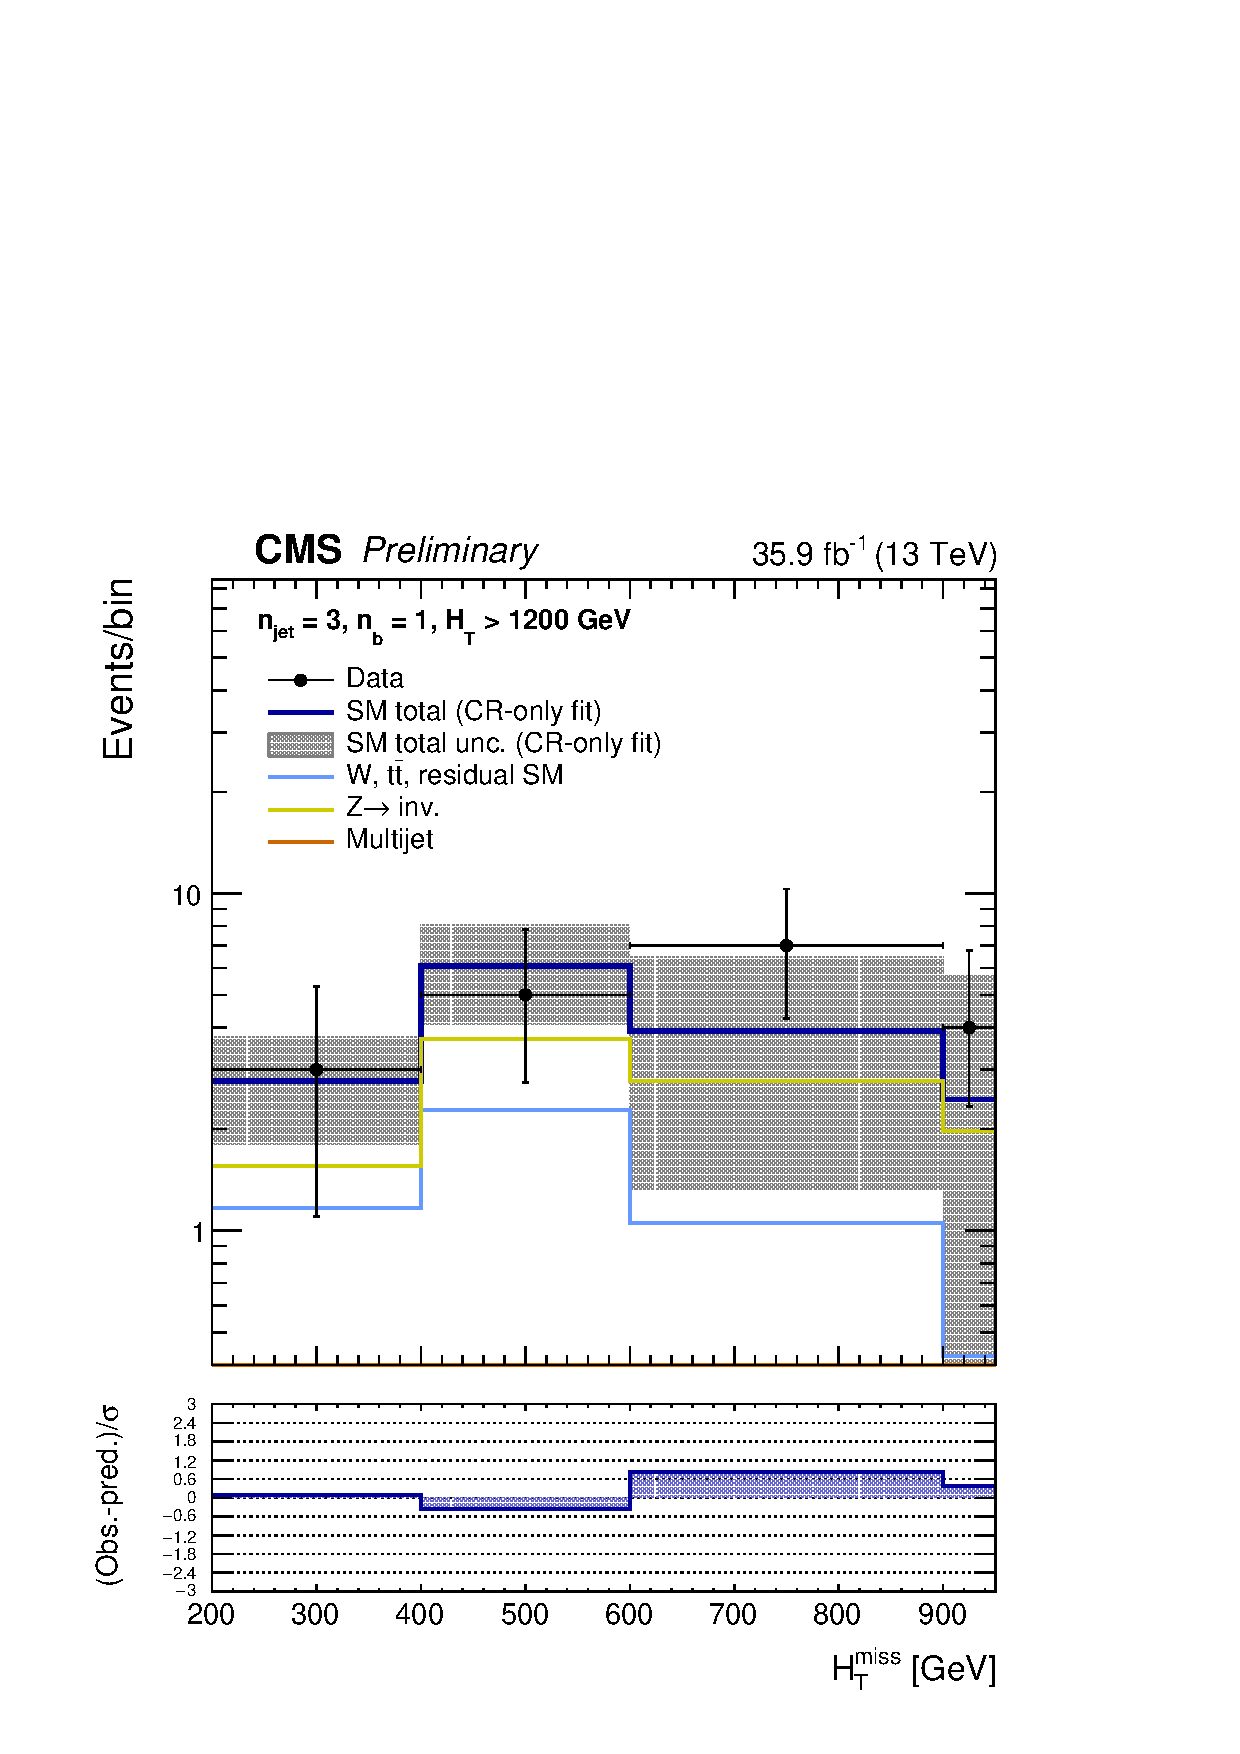
\includegraphics[width=0.49\textwidth]{figures/results/36invfb_preapproval//crfit/shapes//mhtShape_eq1b_eq3j_1200_Inf_crfit.pdf}}\\
    \caption{Event yields observed in data (solid circles) and CR-fit SM expectations with their associated uncertainties (green histogram with shaded band) as a function of \HTmiss based on a sample of events that satisfy $\njet = 3$ and $\nb = 1$, as well as the requirements on \scalht indicated by each sub-figure caption. }
    \label{fig:mhtdim_eq3j_eq1b}
  \end{center}
\end{figure}

\clearpage
\begin{figure}[h!]
  \begin{center}
    \subfigure[$400 < \scalht < 600\GeV$]{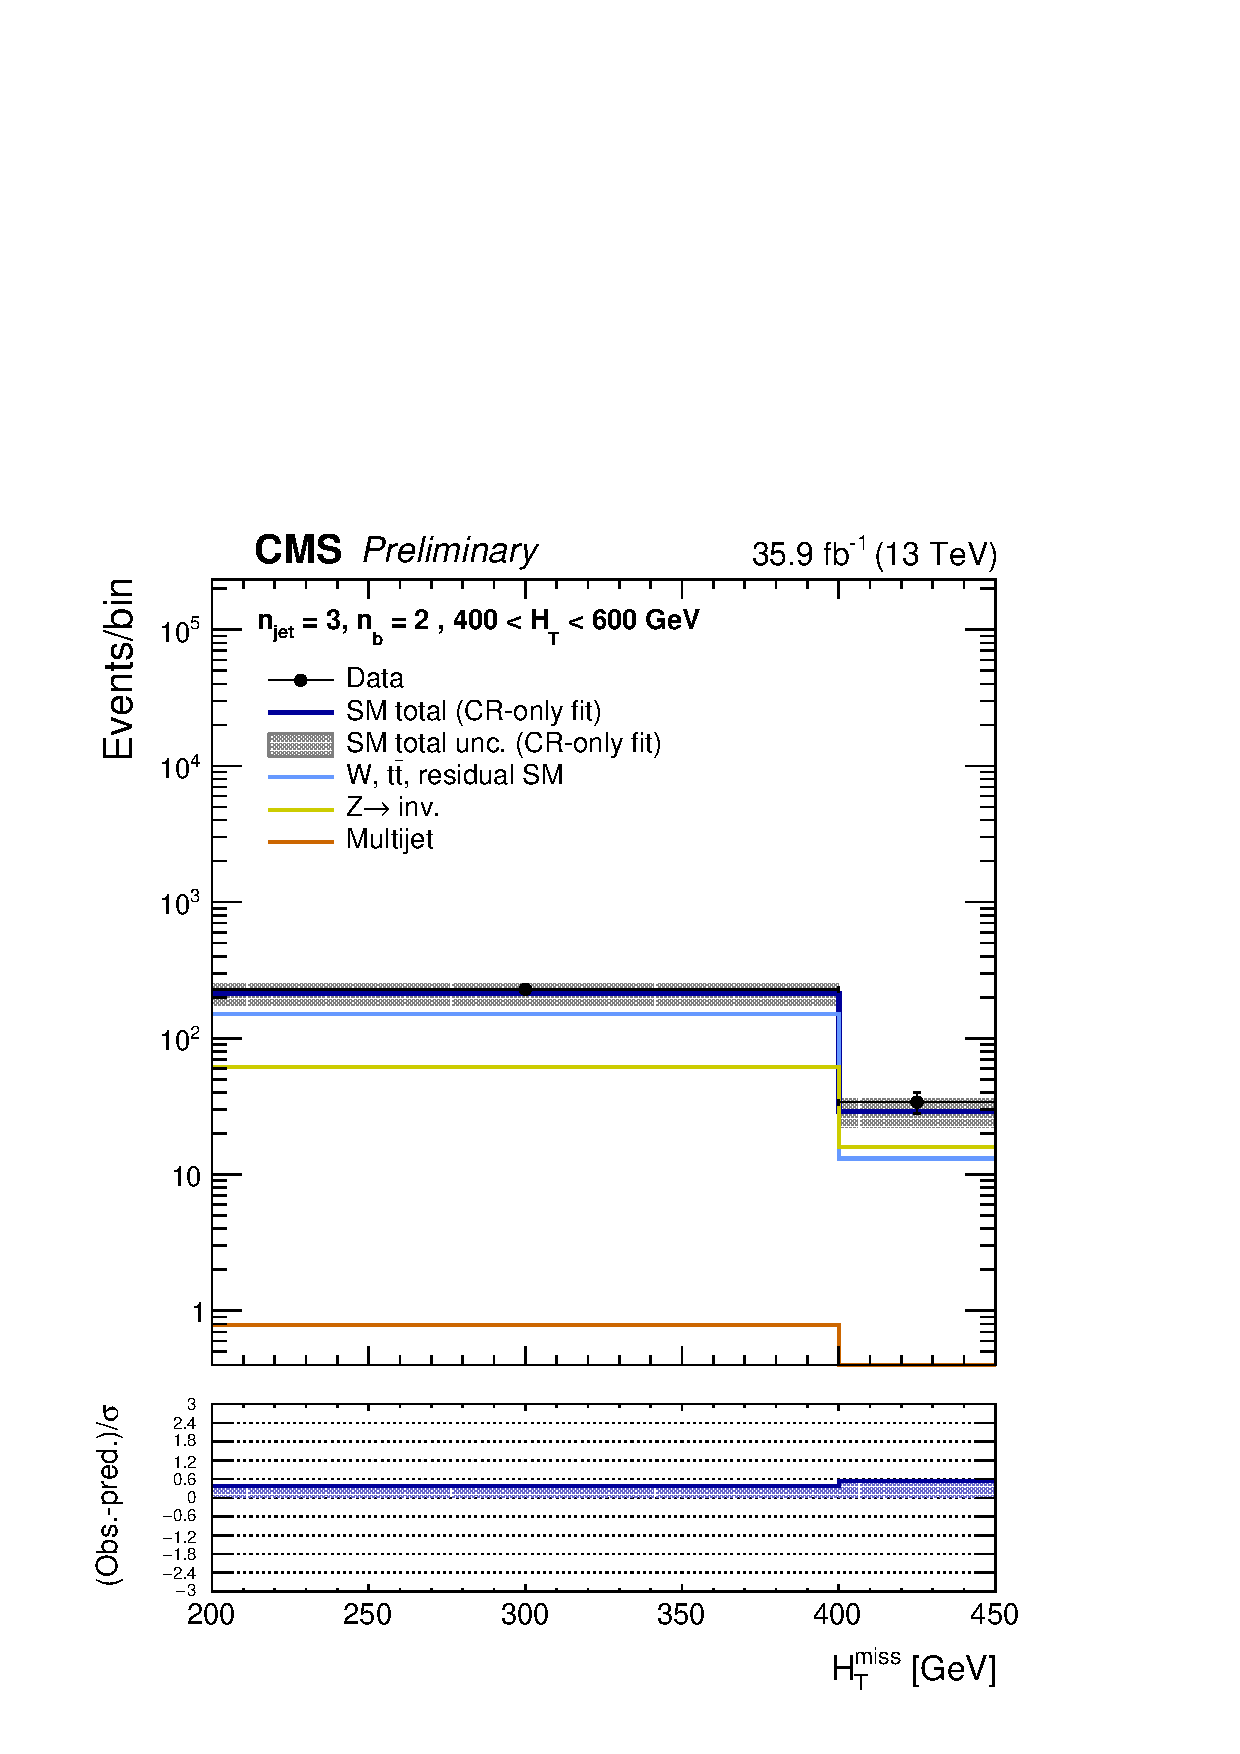
\includegraphics[width=0.49\textwidth]{figures/results/36invfb_preapproval//crfit/shapes//mhtShape_eq2b_eq3j_400_600_crfit.pdf}}
    \subfigure[$600 < \scalht < 900\GeV$]{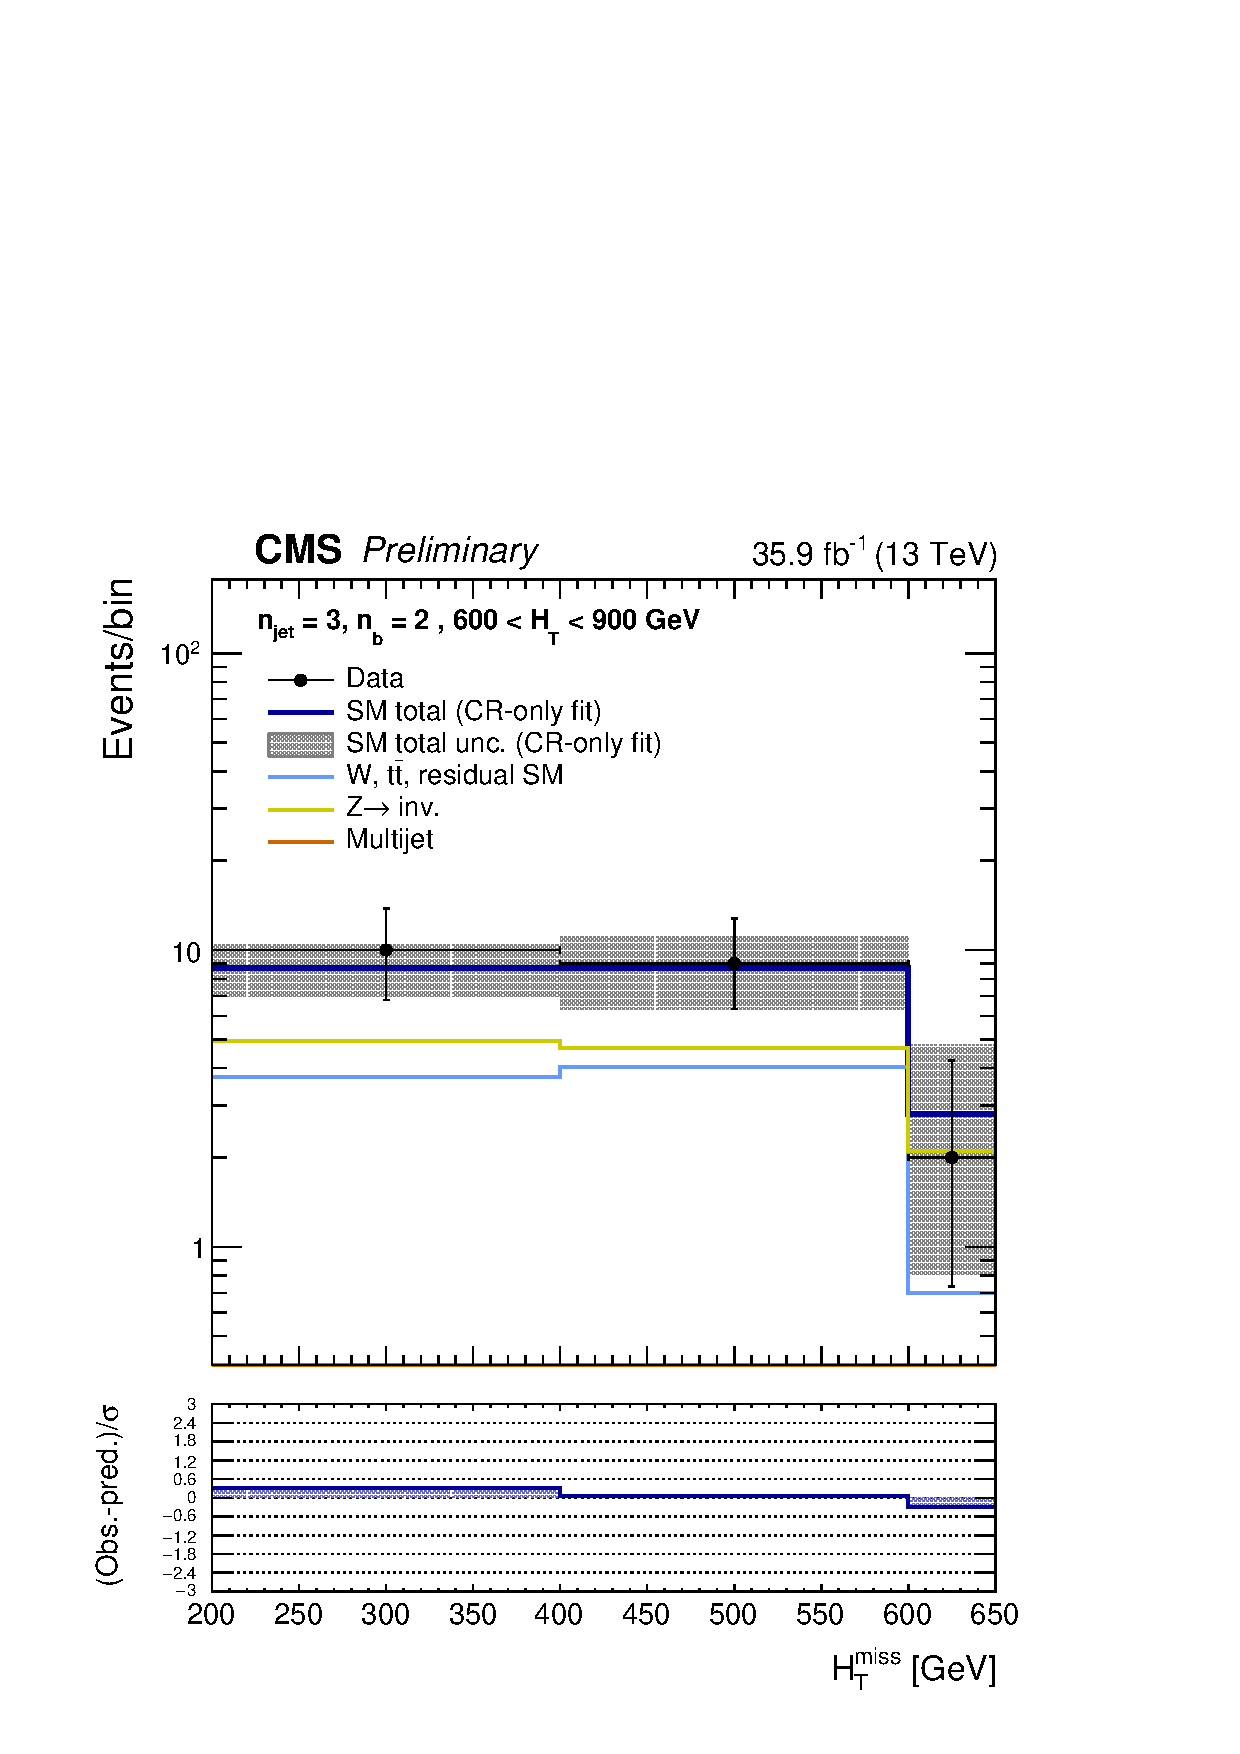
\includegraphics[width=0.49\textwidth]{figures/results/36invfb_preapproval//crfit/shapes//mhtShape_eq2b_eq3j_600_900_crfit.pdf}}\\
    \subfigure[$900 < \scalht < 1200\GeV$]{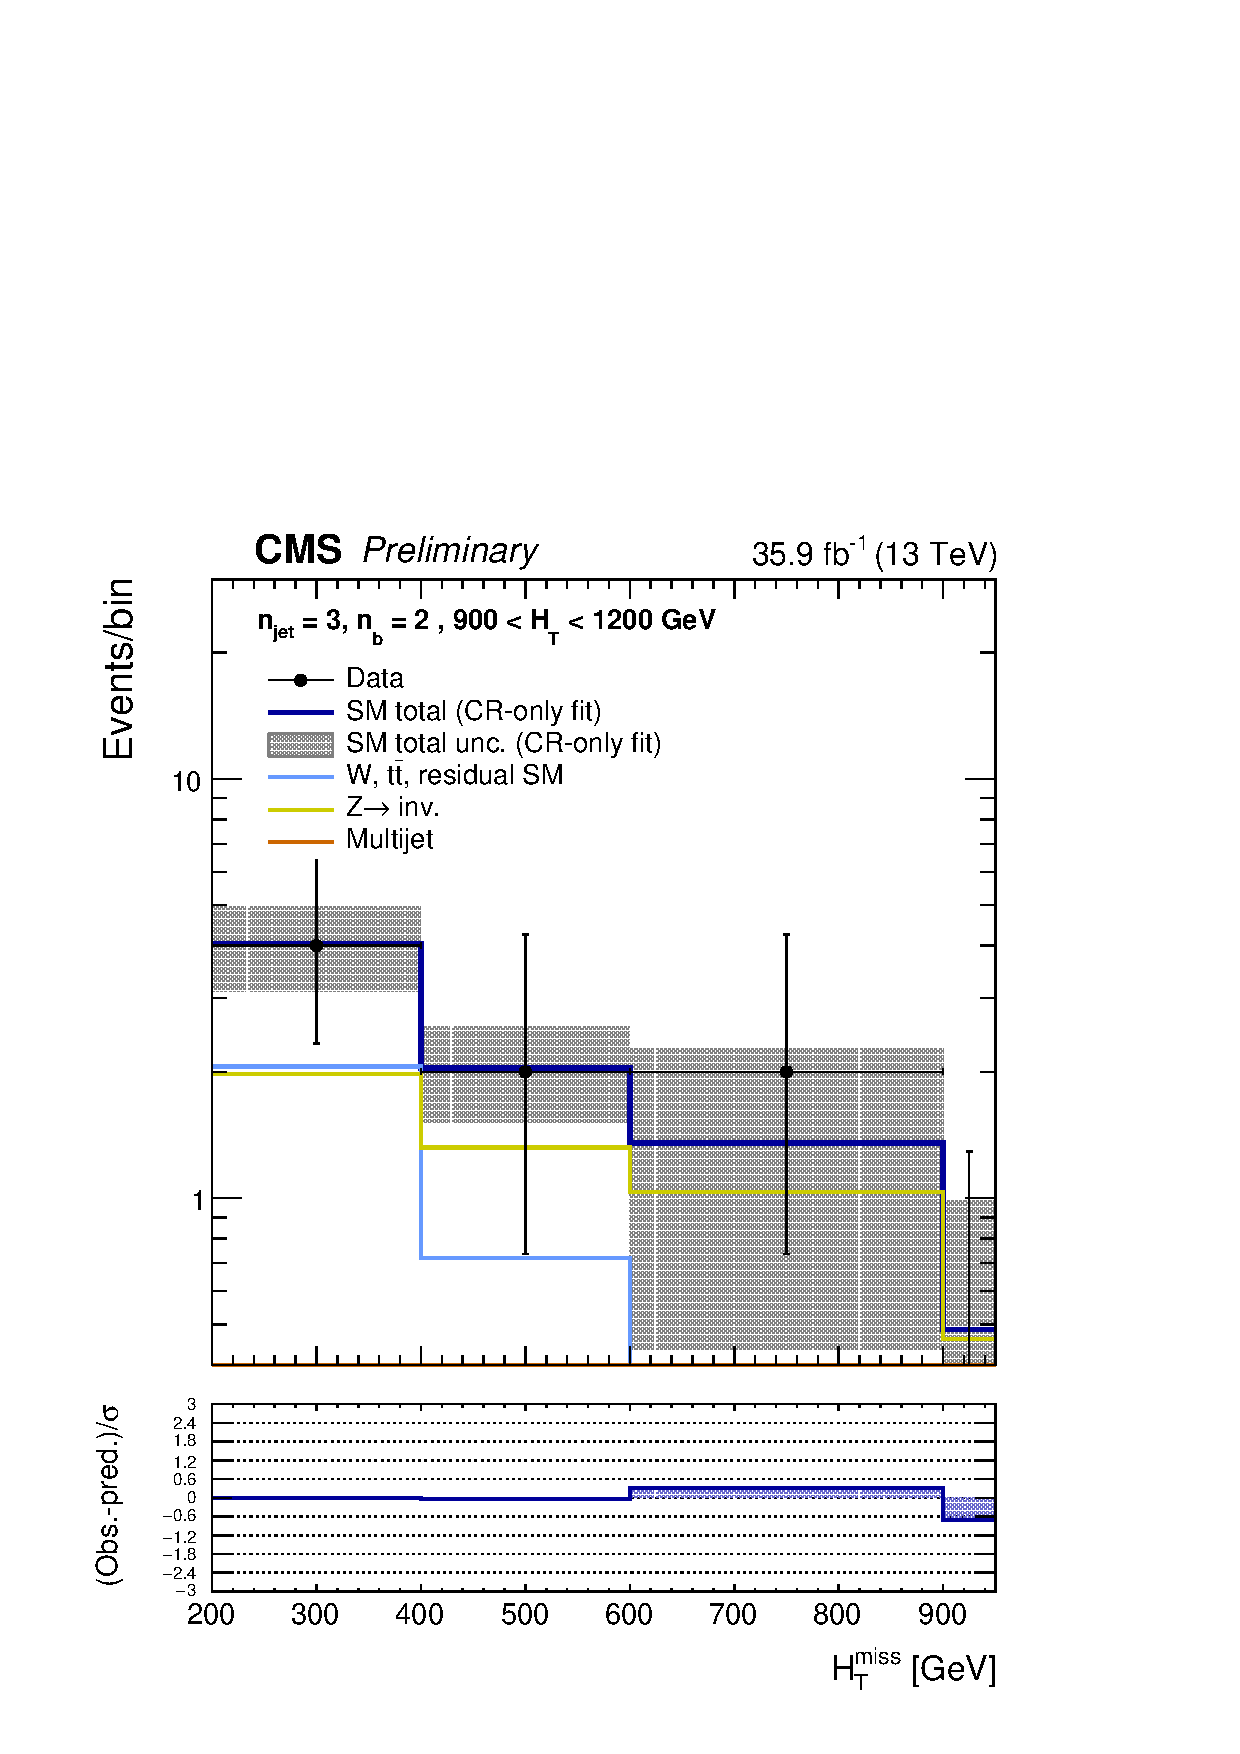
\includegraphics[width=0.49\textwidth]{figures/results/36invfb_preapproval//crfit/shapes//mhtShape_eq2b_eq3j_900_1200_crfit.pdf}}
    \subfigure[$\scalht > 1200\GeV$]{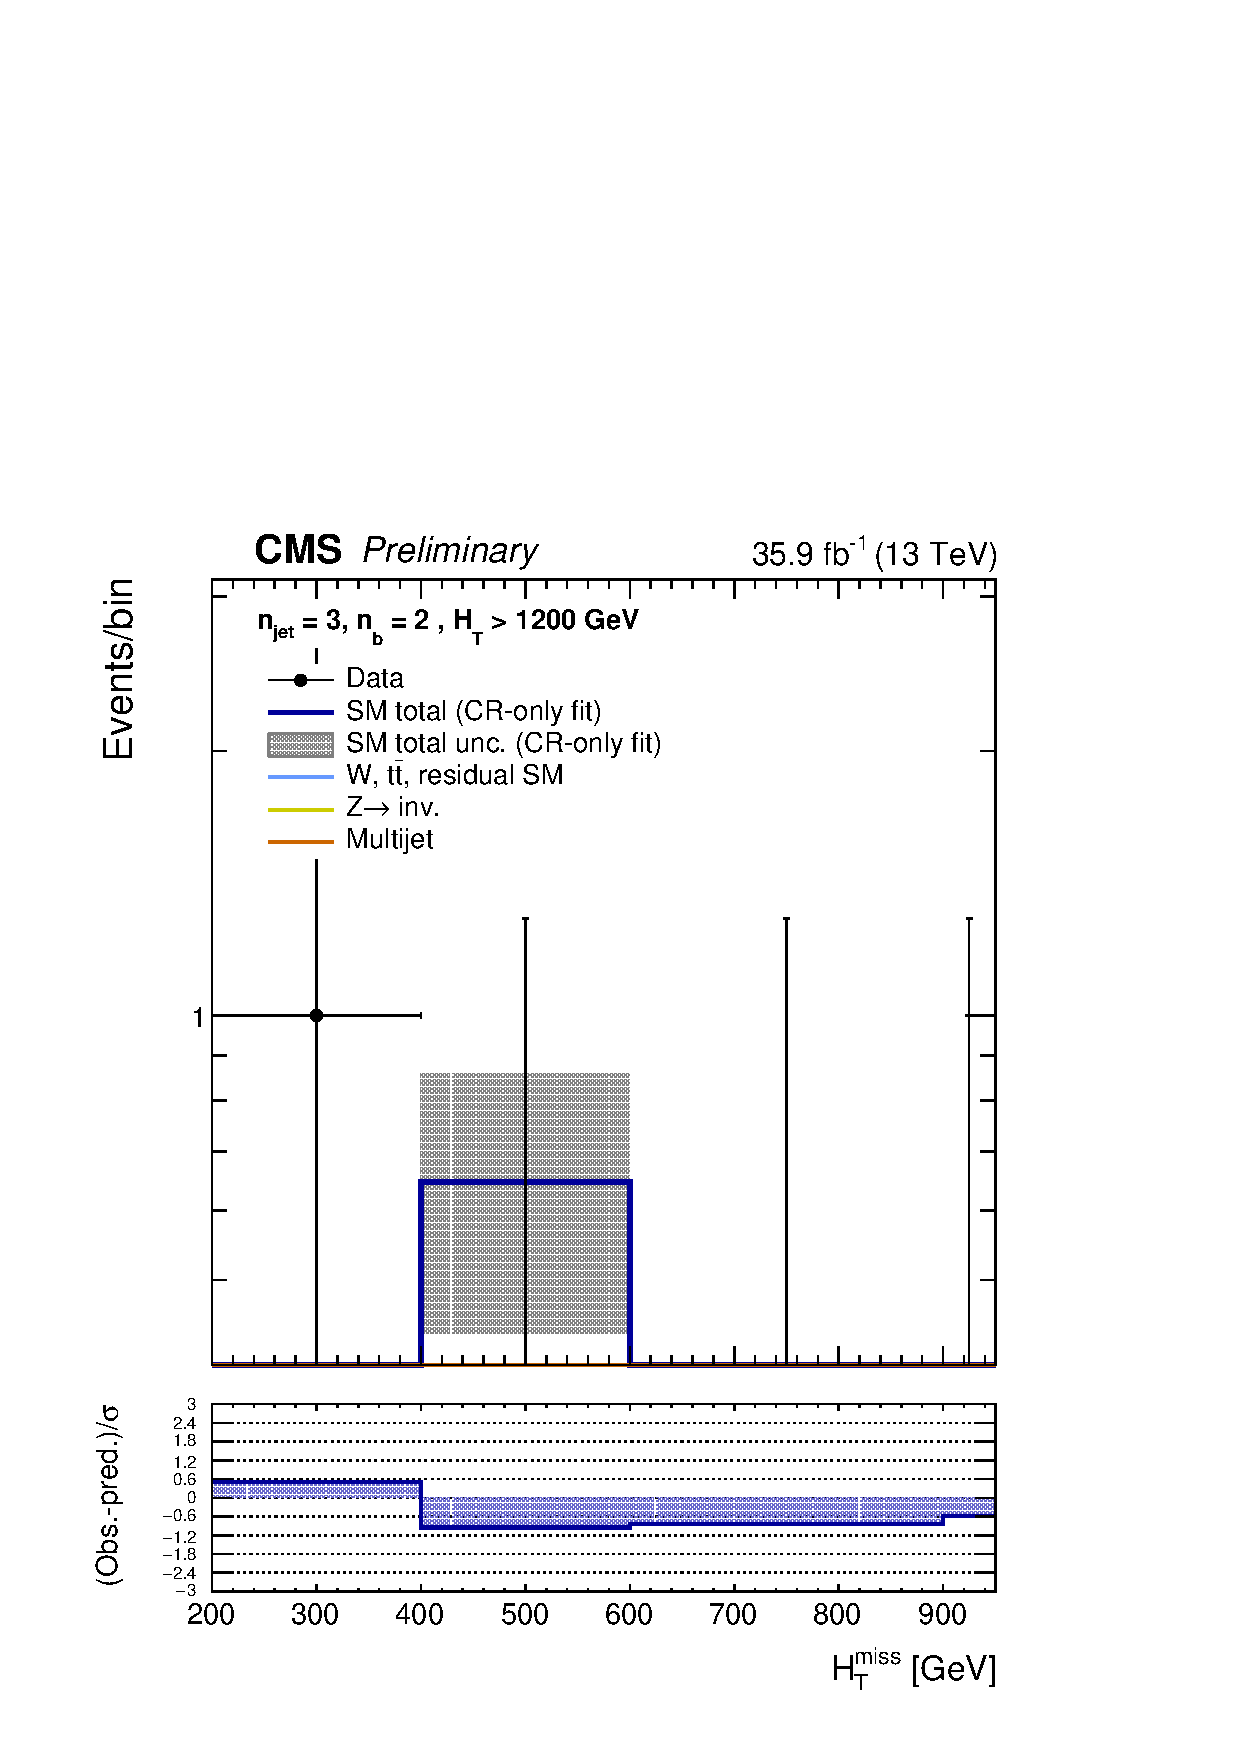
\includegraphics[width=0.49\textwidth]{figures/results/36invfb_preapproval//crfit/shapes//mhtShape_eq2b_eq3j_1200_Inf_crfit.pdf}}\\
    \caption{Event yields observed in data (solid circles) and CR-fit SM expectations with their associated uncertainties (green histogram with shaded band) as a function of \HTmiss based on a sample of events that satisfy $\njet = 3$ and $\nb = 2$, as well as the requirements on \scalht indicated by each sub-figure caption. }
    \label{fig:mhtdim_eq3j_eq2b}
  \end{center}
\end{figure}

\clearpage
\begin{figure}[h!]
  \begin{center}
    \subfigure[$400 < \scalht < 600\GeV$]{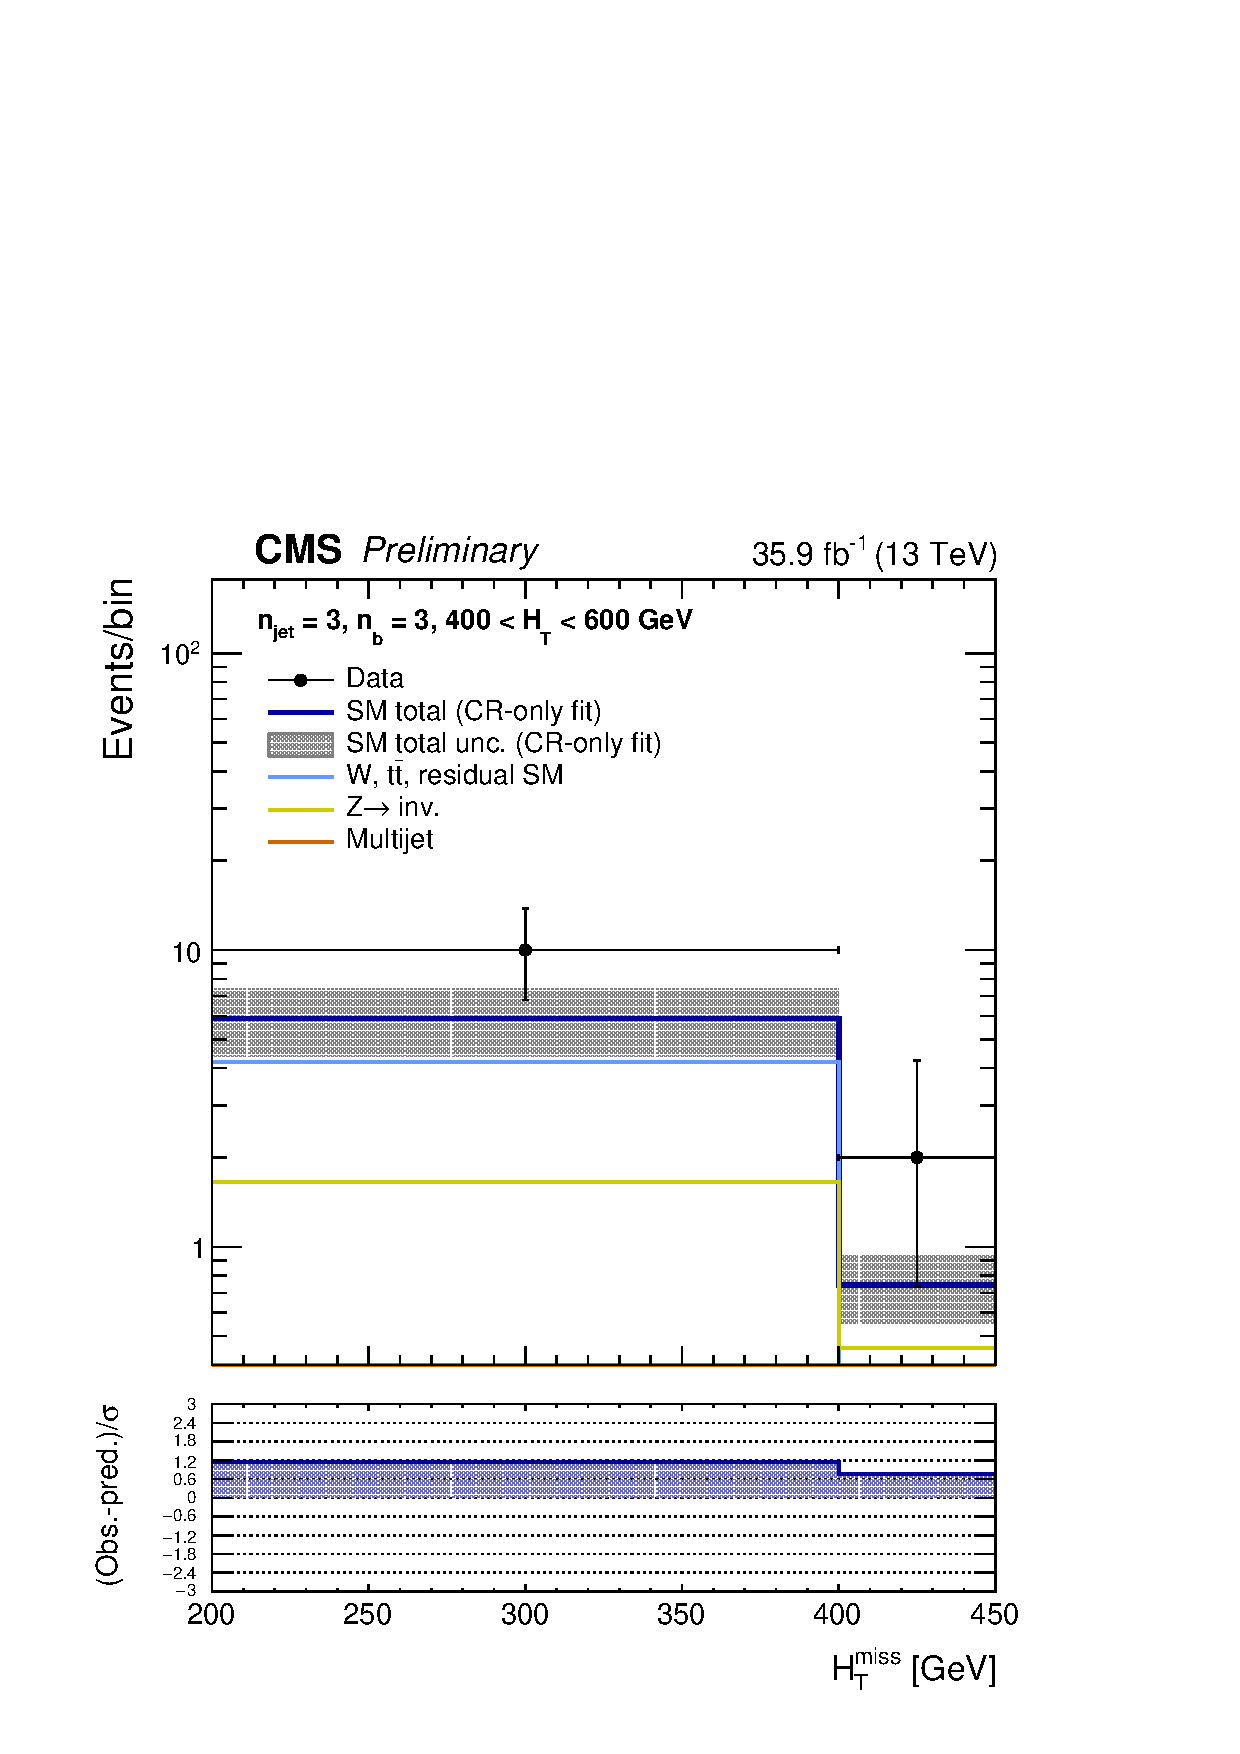
\includegraphics[width=0.49\textwidth]{figures/results/36invfb_preapproval//crfit/shapes//mhtShape_eq3b_eq3j_400_600_crfit.pdf}}
    \caption{Event yields observed in data (solid circles) and CR-fit SM expectations with their associated uncertainties (green histogram with shaded band) as a function of \HTmiss based on a sample of events that satisfy $\njet = 3$ and $\nb = 3$, as well as the requirements on \scalht indicated by each sub-figure caption. }
    \label{fig:mhtdim_eq3j_eq3b}
  \end{center}
\end{figure}

\clearpage
\begin{figure}[h!]
  \begin{center}
    \subfigure[$400 < \scalht < 600\GeV$]{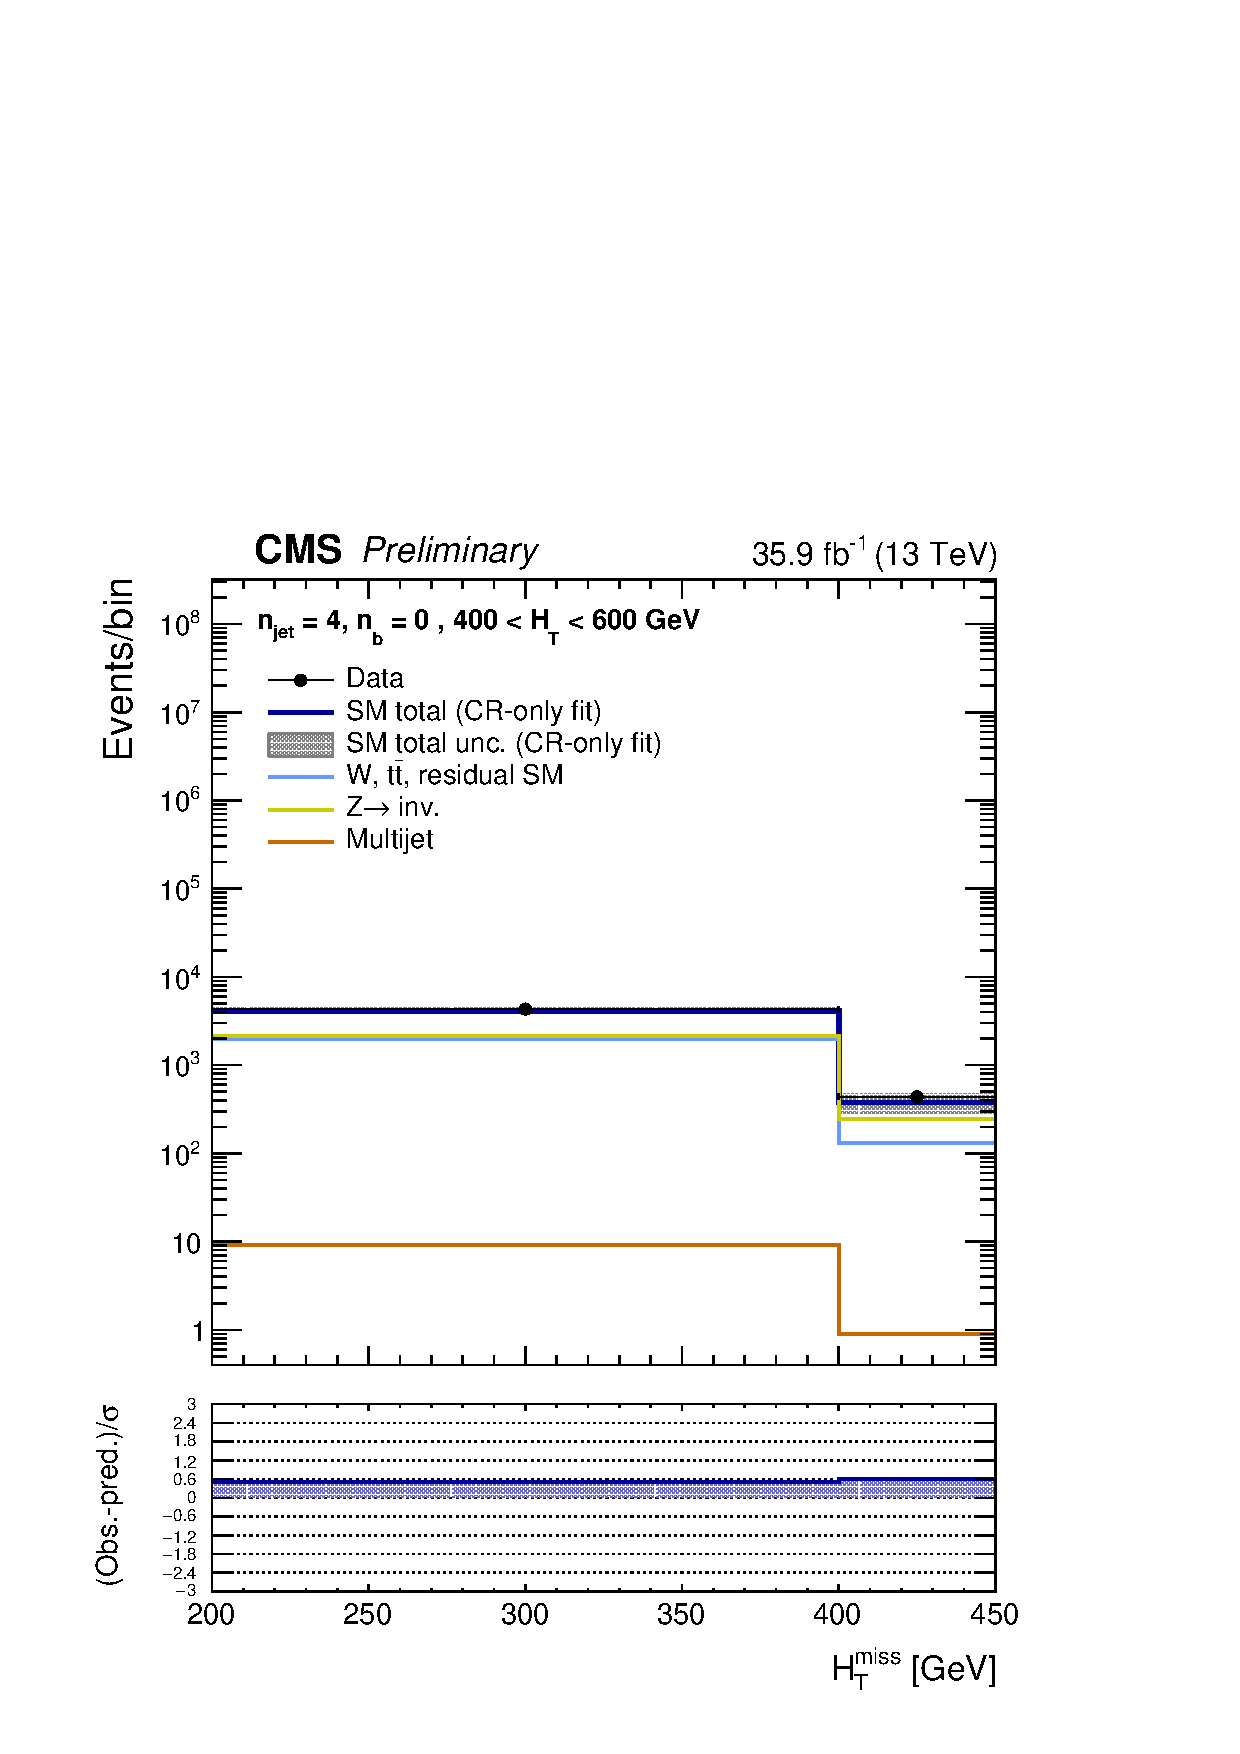
\includegraphics[width=0.49\textwidth]{figures/results/36invfb_preapproval//crfit/shapes//mhtShape_eq0b_eq4j_400_600_crfit.pdf}}
    \subfigure[$600 < \scalht < 900\GeV$]{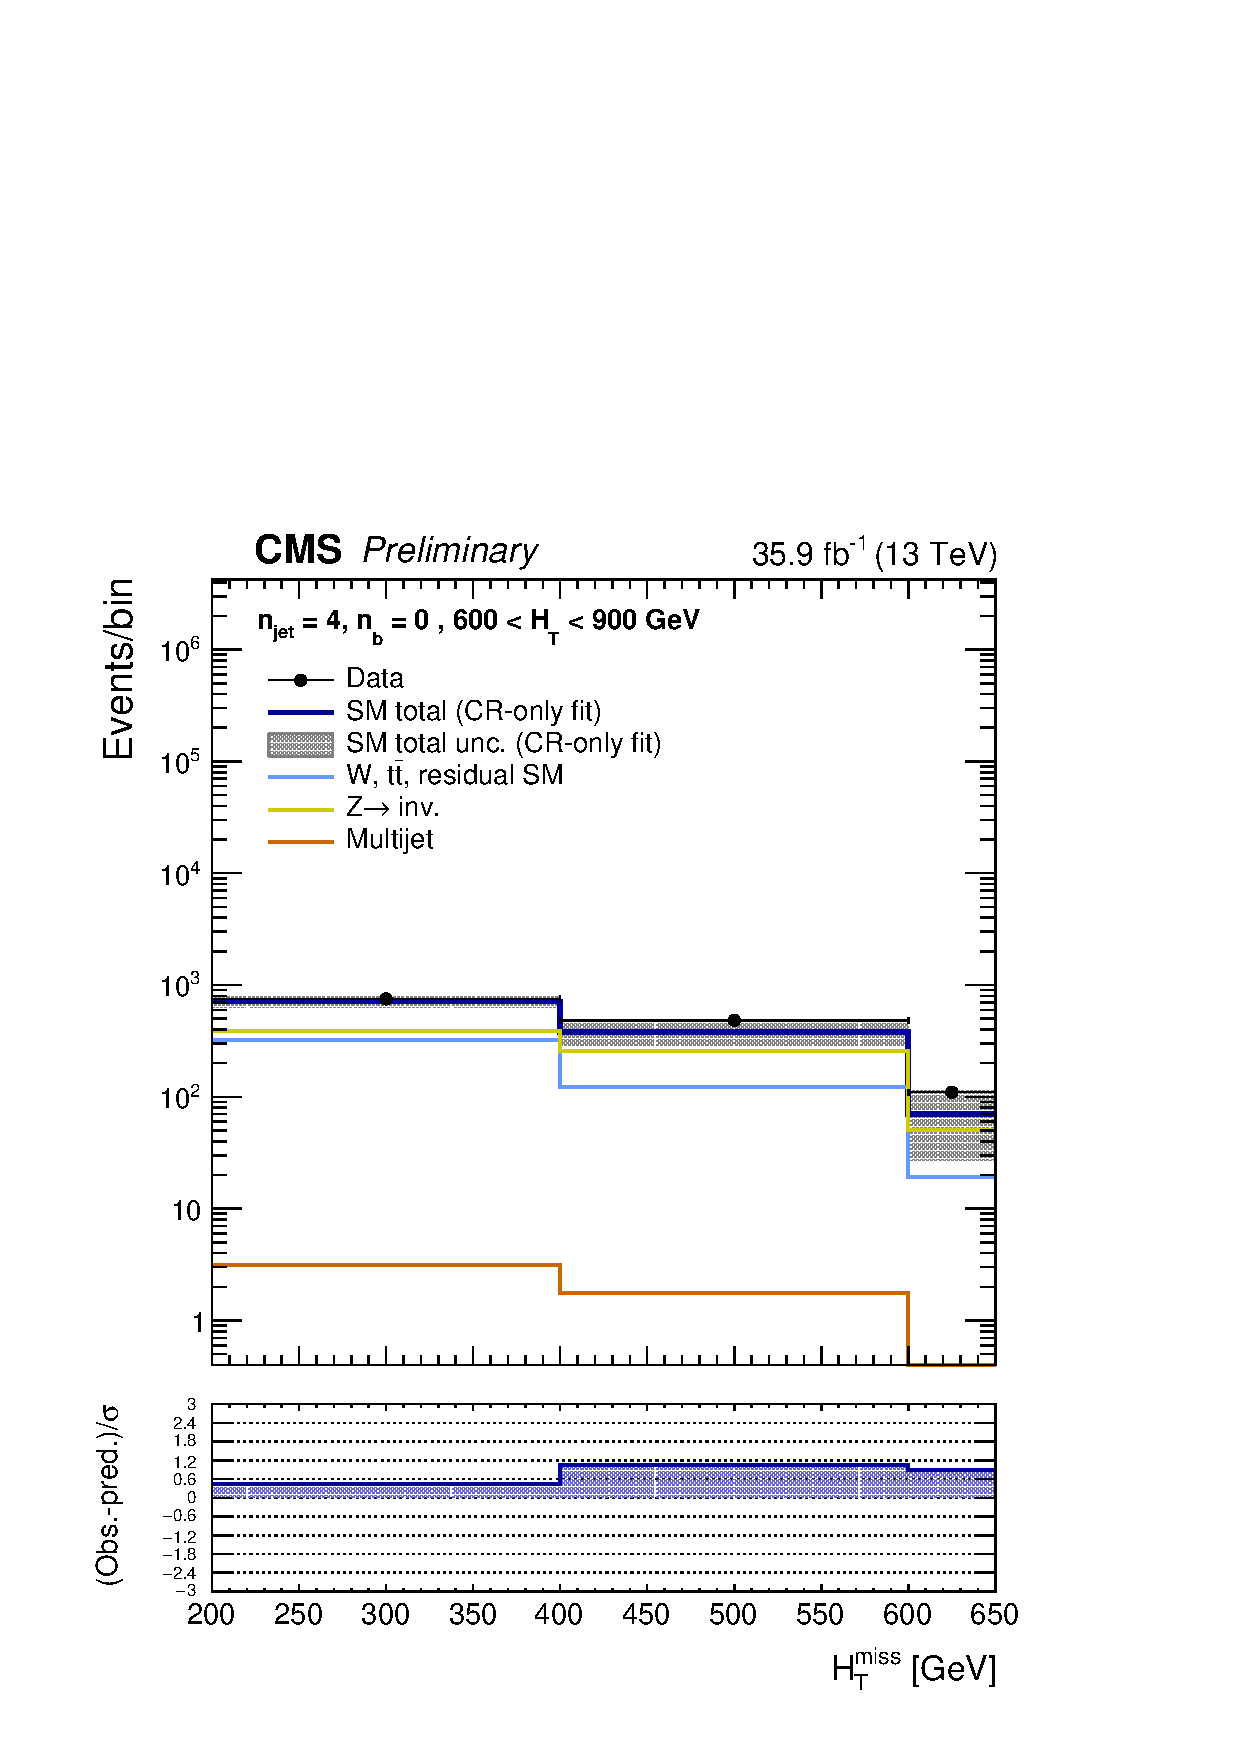
\includegraphics[width=0.49\textwidth]{figures/results/36invfb_preapproval//crfit/shapes//mhtShape_eq0b_eq4j_600_900_crfit.pdf}}\\
    \subfigure[$900 < \scalht < 1200\GeV$]{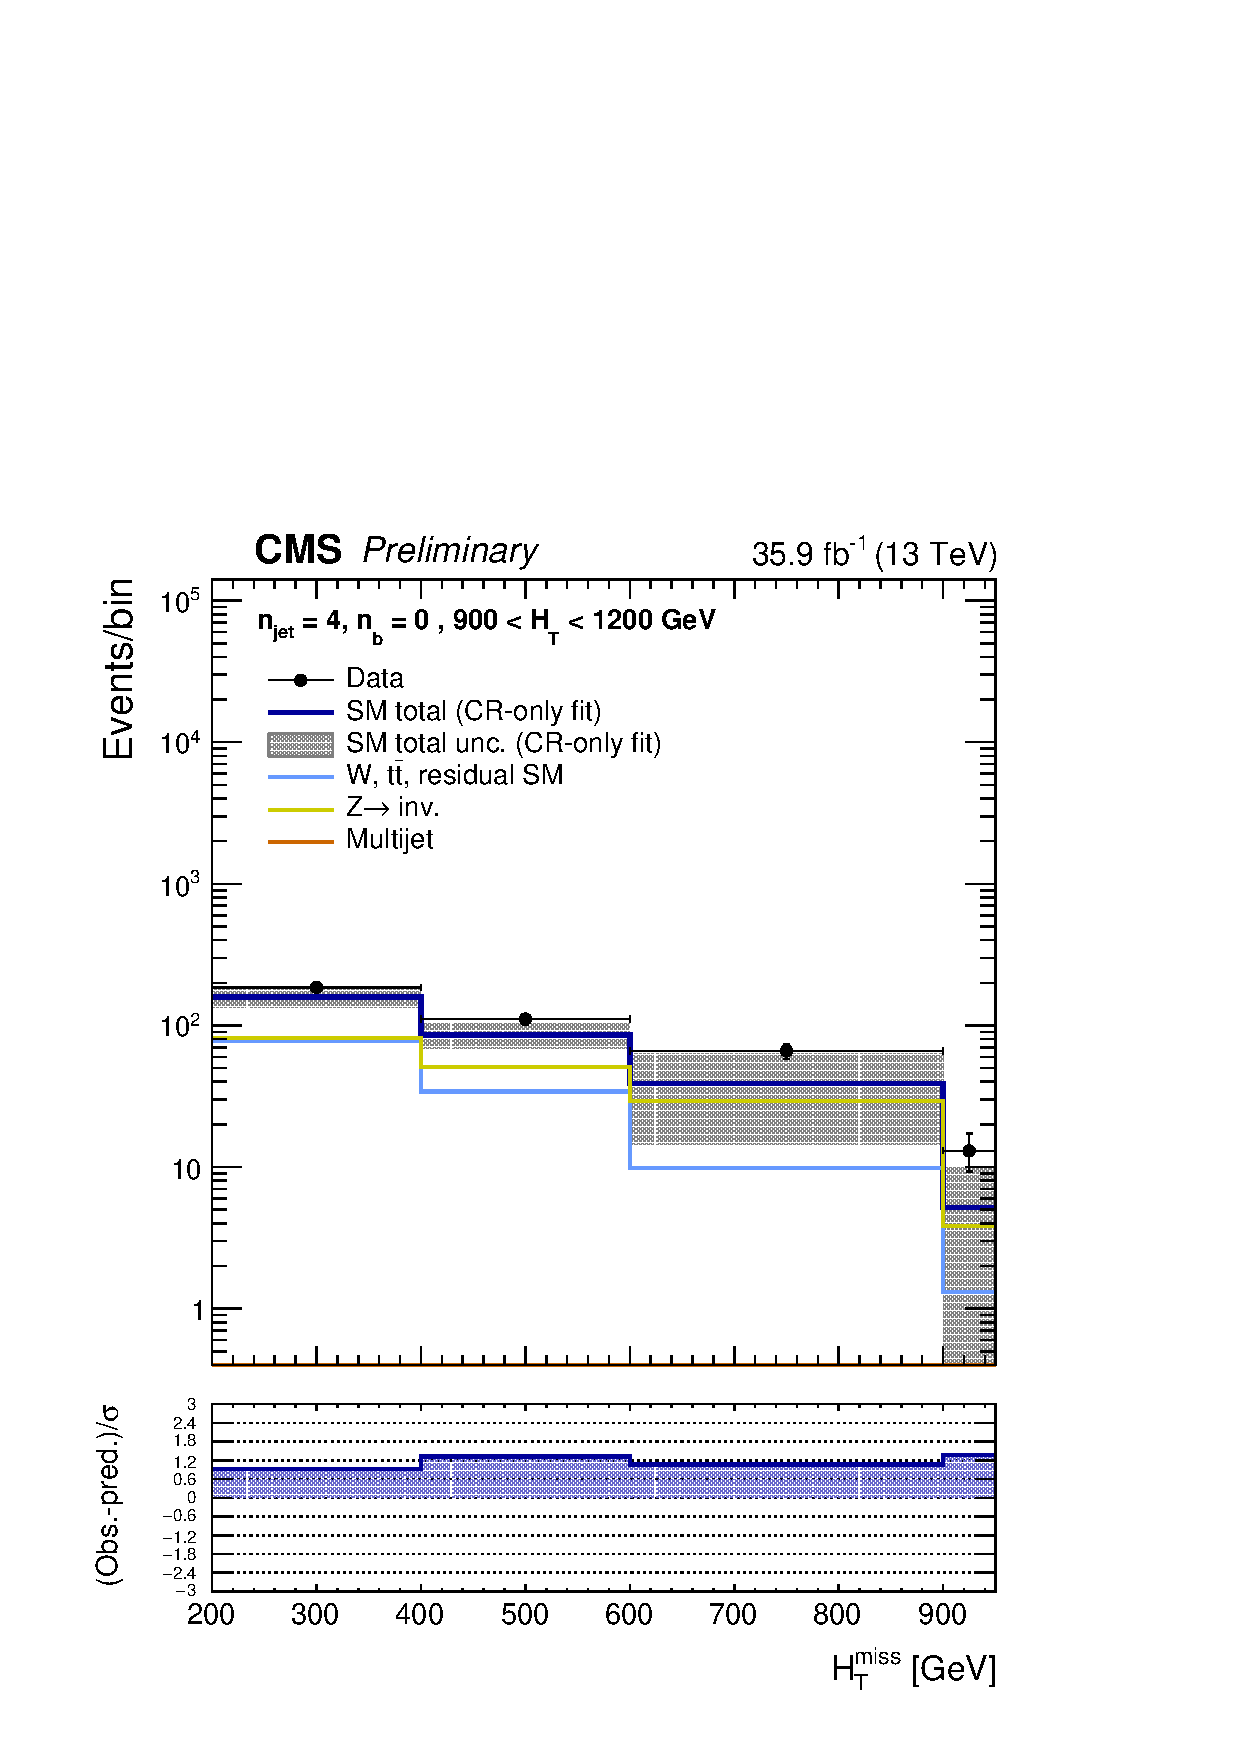
\includegraphics[width=0.49\textwidth]{figures/results/36invfb_preapproval//crfit/shapes//mhtShape_eq0b_eq4j_900_1200_crfit.pdf}}
    \subfigure[$\scalht > 1200\GeV$]{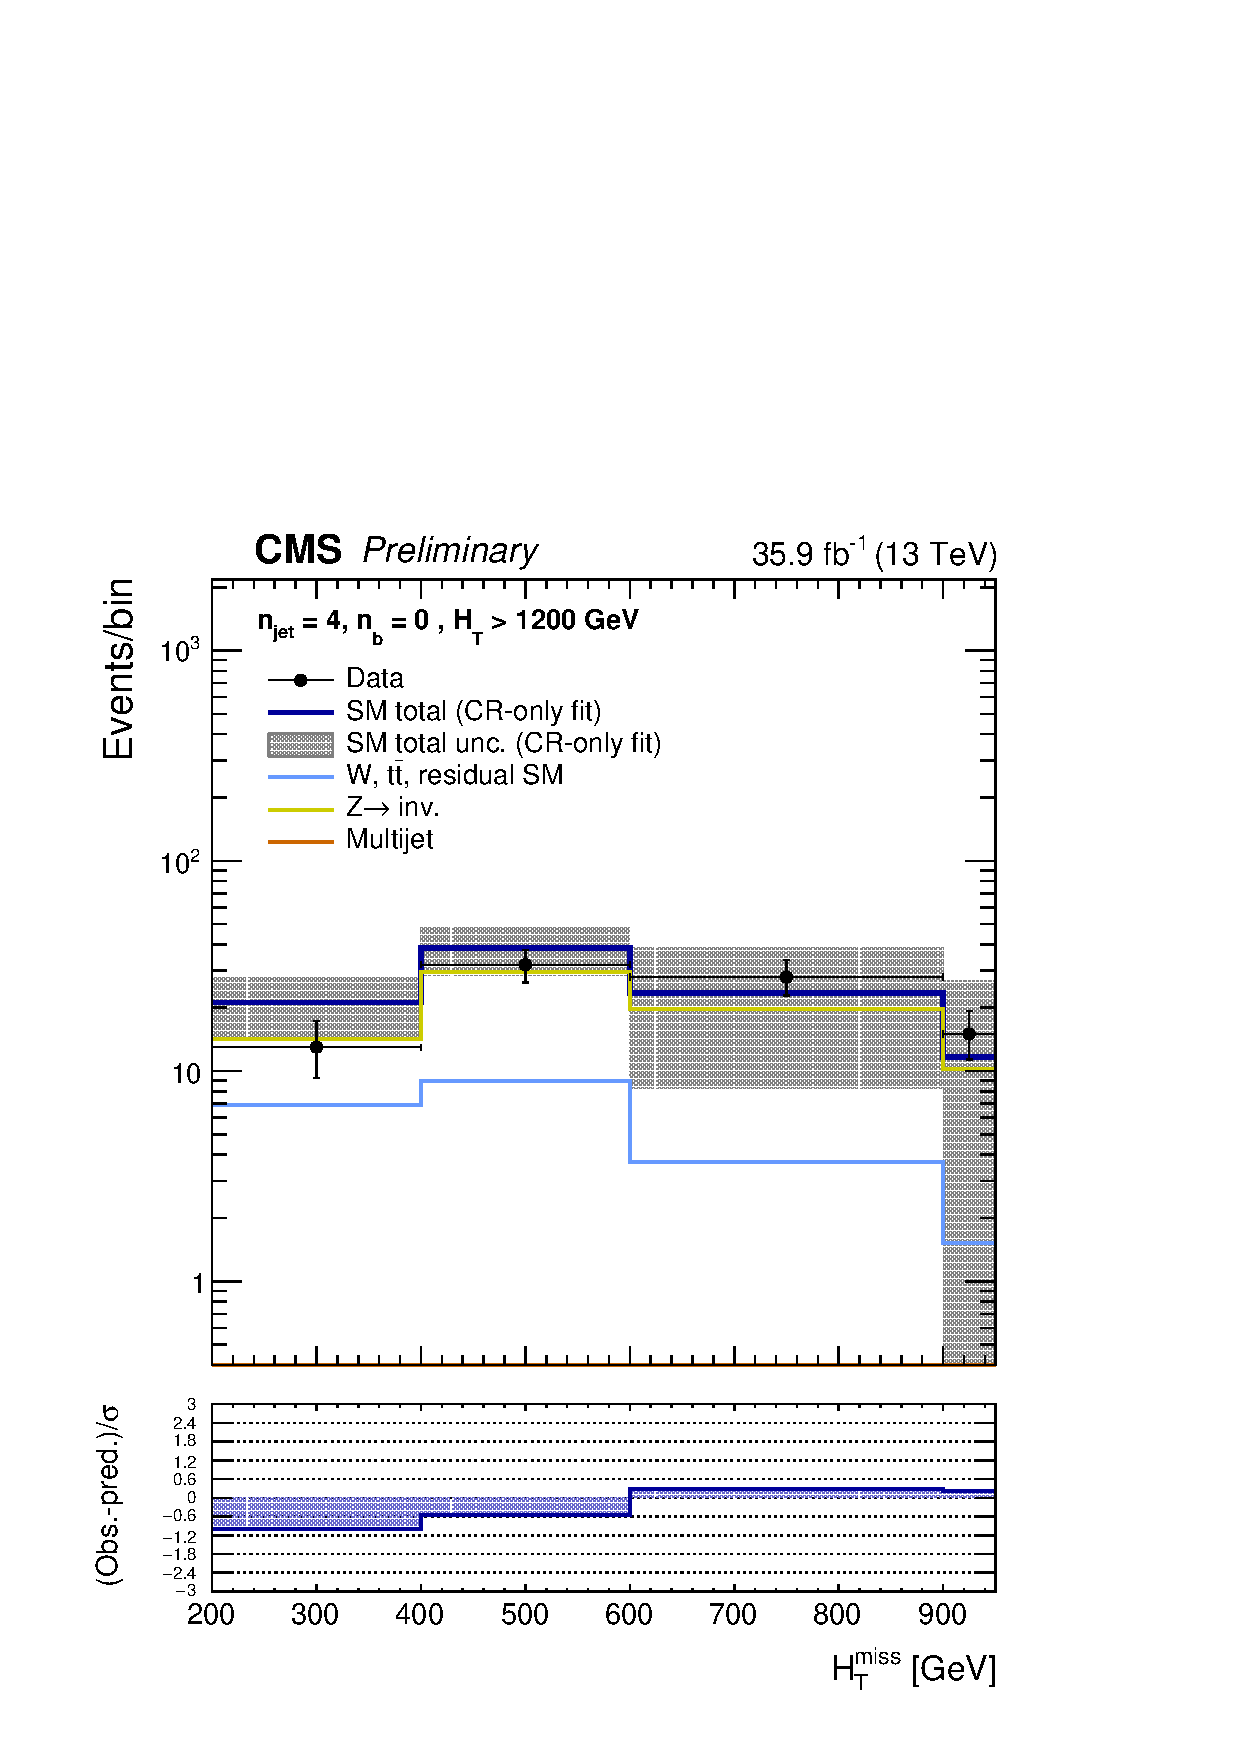
\includegraphics[width=0.49\textwidth]{figures/results/36invfb_preapproval//crfit/shapes//mhtShape_eq0b_eq4j_1200_Inf_crfit.pdf}}\\
    \caption{Event yields observed in data (solid circles) and CR-fit SM expectations with their associated uncertainties (green histogram with shaded band) as a function of \HTmiss based on a sample of events that satisfy $\njet = 4$ and $\nb = 0$, as well as the requirements on \scalht indicated by each sub-figure caption. }
    \label{fig:mhtdim_eq4j_eq0b}
  \end{center}
\end{figure}

\clearpage
\begin{figure}[h!]
  \begin{center}
    \subfigure[$400 < \scalht < 600\GeV$]{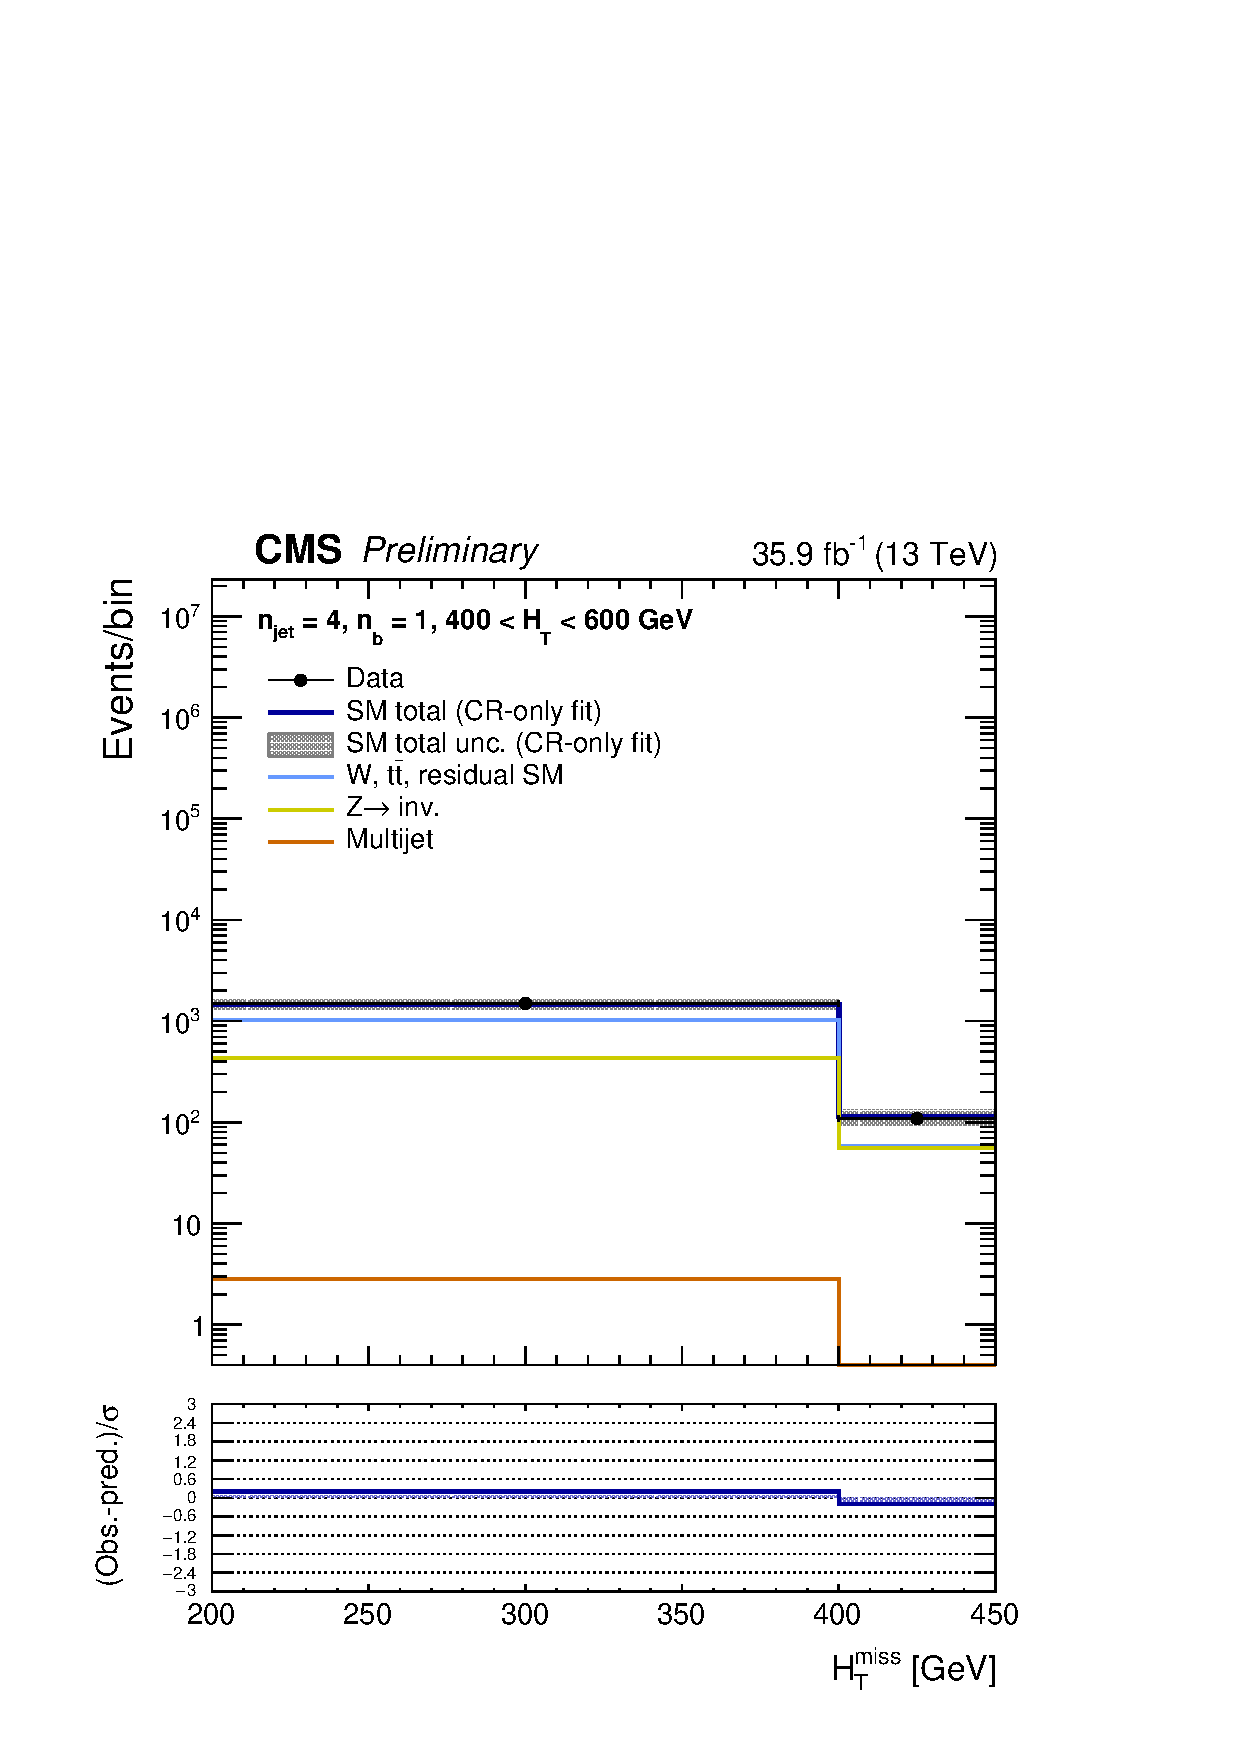
\includegraphics[width=0.49\textwidth]{figures/results/36invfb_preapproval//crfit/shapes//mhtShape_eq1b_eq4j_400_600_crfit.pdf}}
    \subfigure[$600 < \scalht < 900\GeV$]{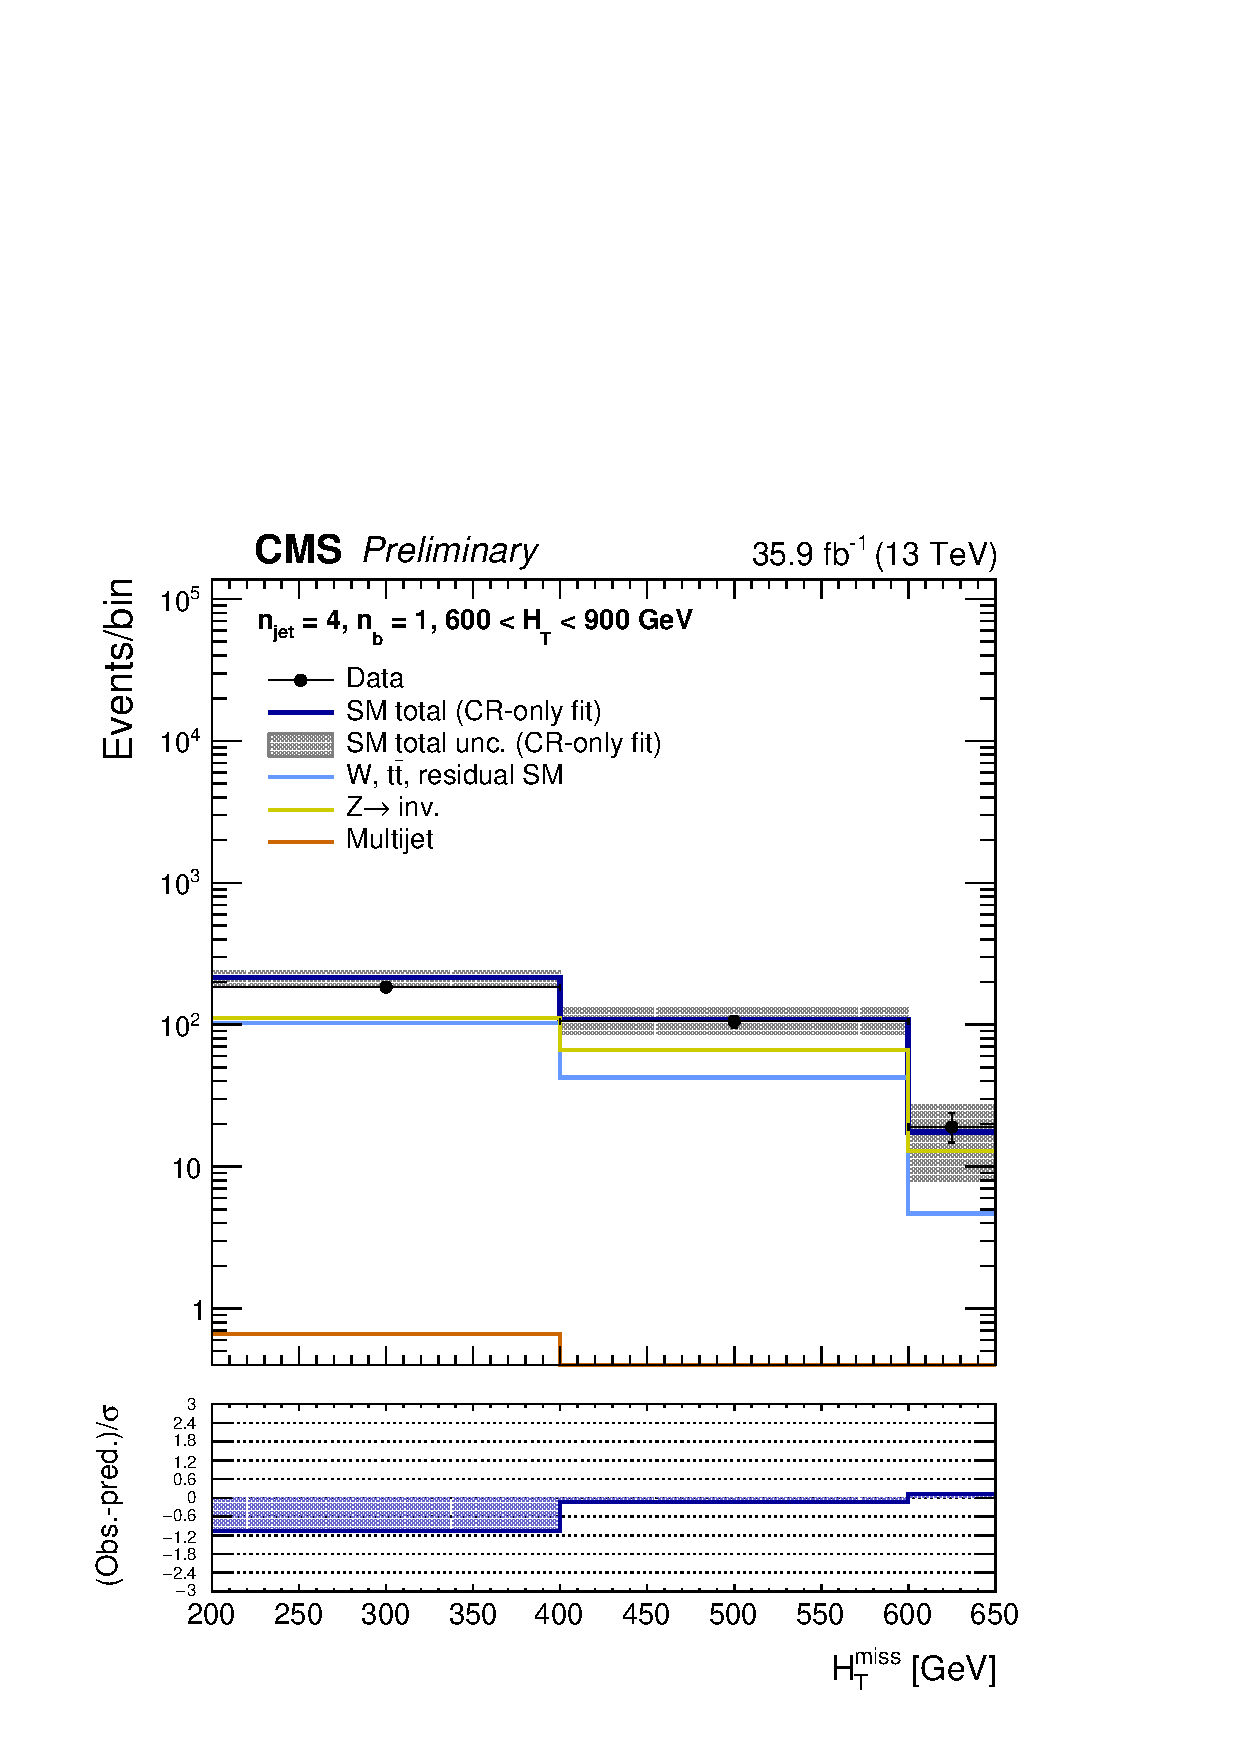
\includegraphics[width=0.49\textwidth]{figures/results/36invfb_preapproval//crfit/shapes//mhtShape_eq1b_eq4j_600_900_crfit.pdf}}\\
    \subfigure[$900 < \scalht < 1200\GeV$]{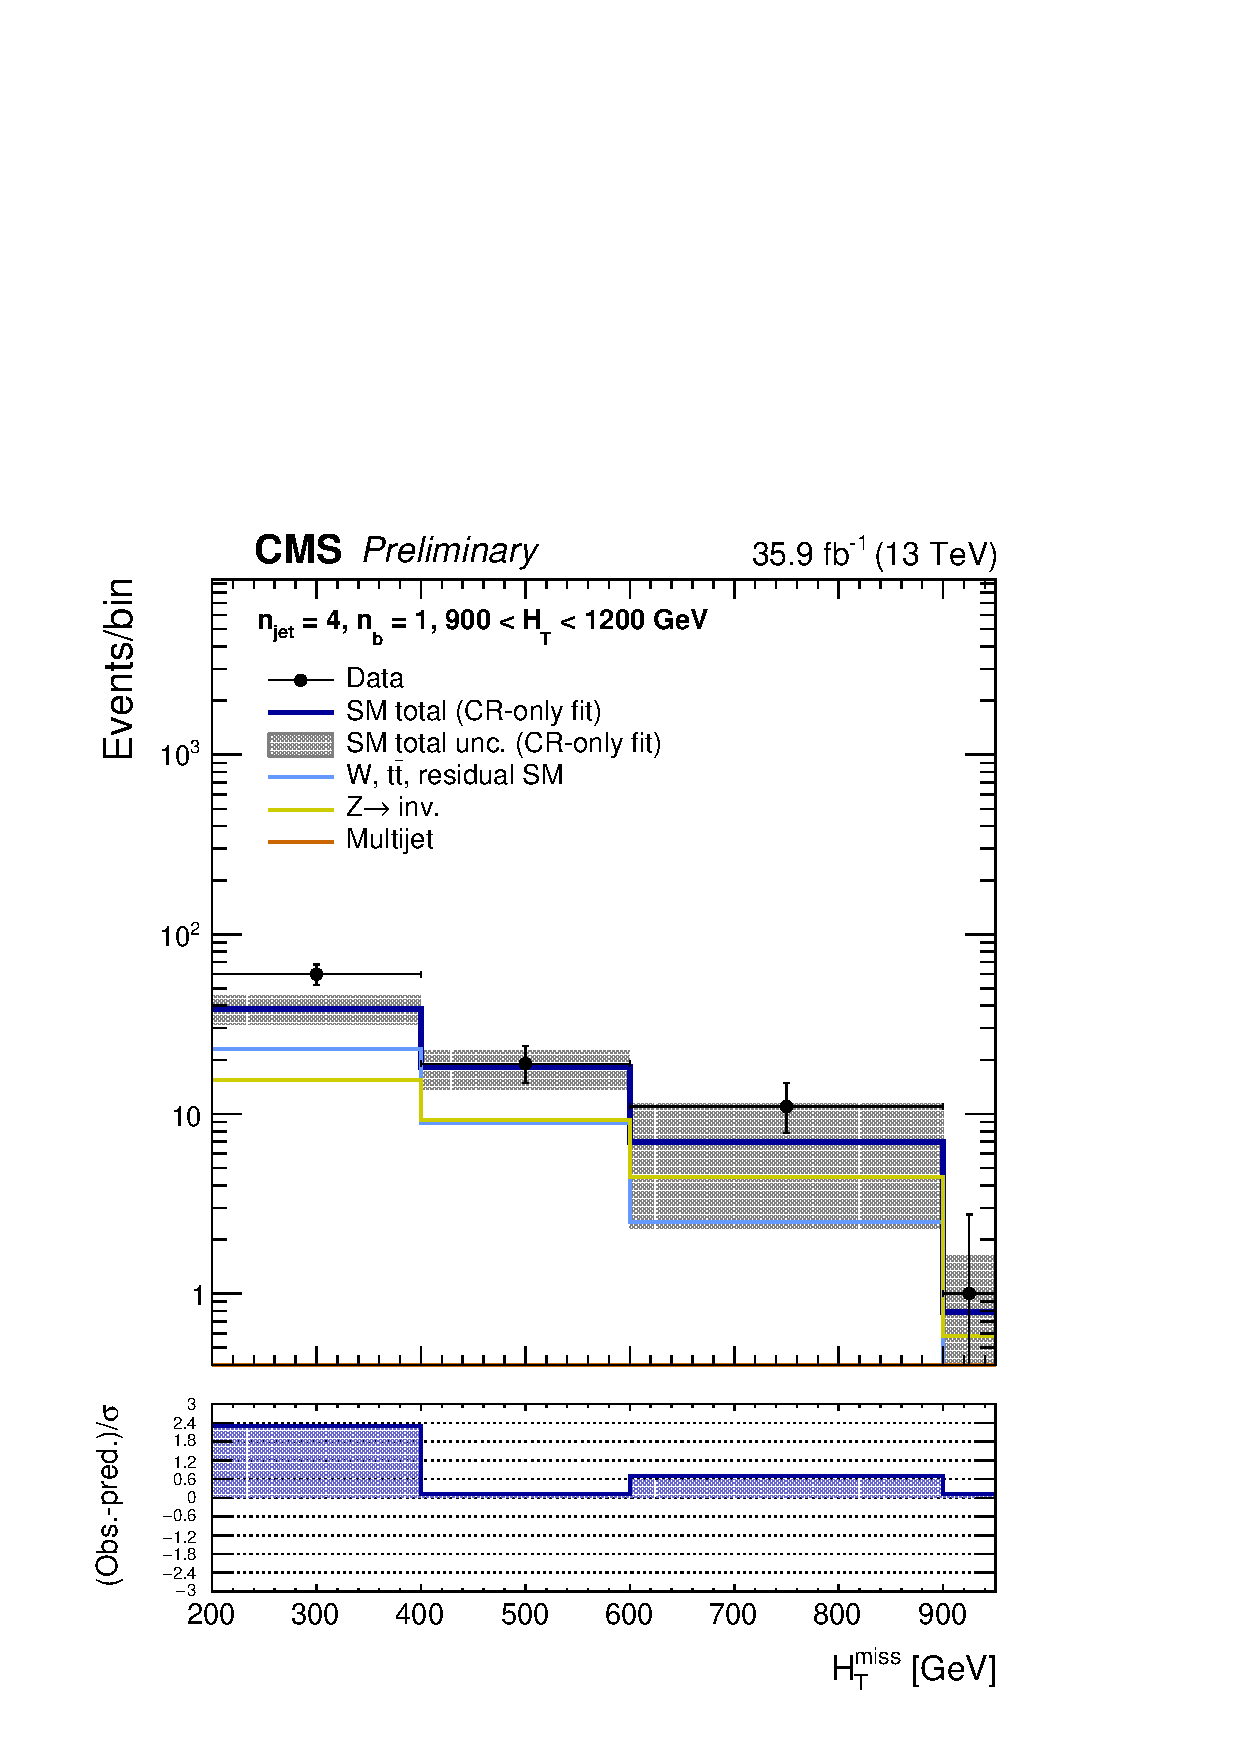
\includegraphics[width=0.49\textwidth]{figures/results/36invfb_preapproval//crfit/shapes//mhtShape_eq1b_eq4j_900_1200_crfit.pdf}}
    \subfigure[$\scalht > 1200\GeV$]{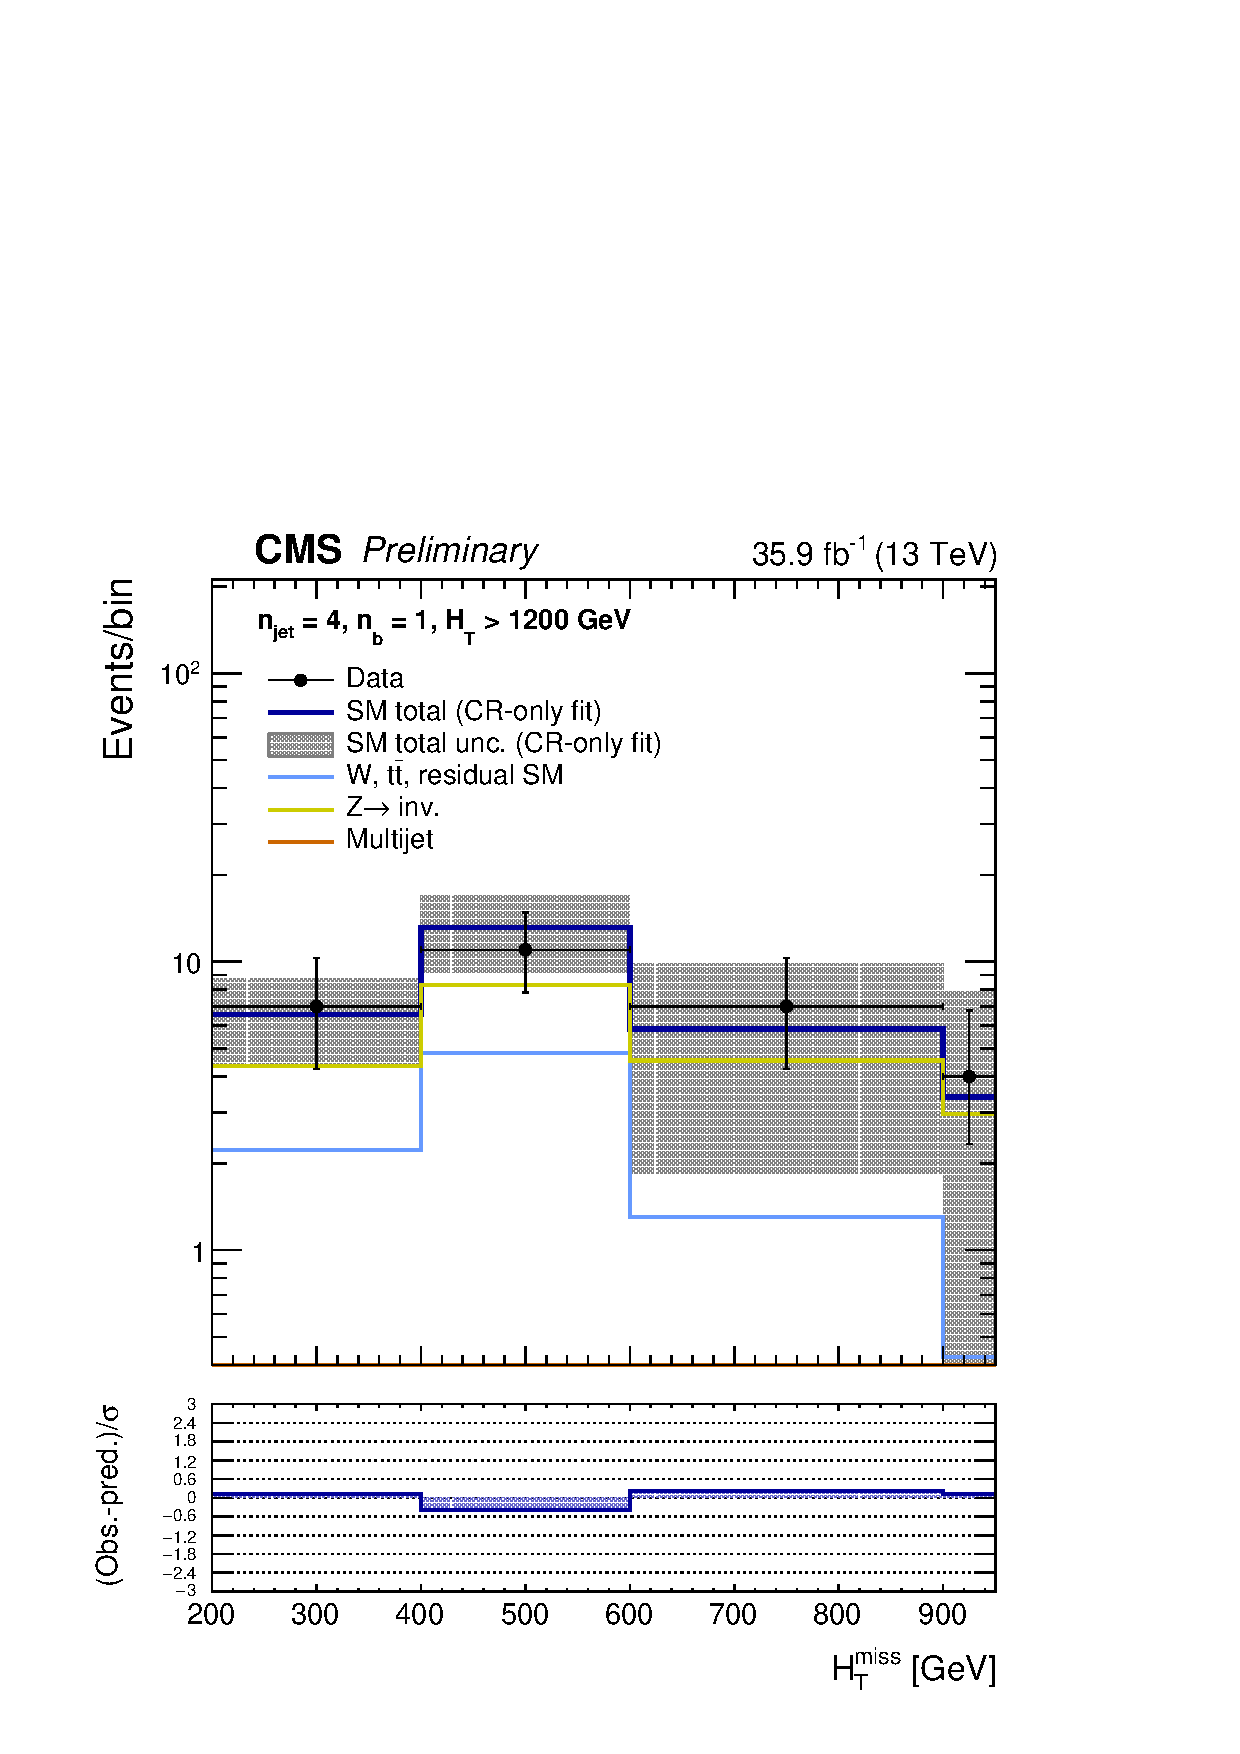
\includegraphics[width=0.49\textwidth]{figures/results/36invfb_preapproval//crfit/shapes//mhtShape_eq1b_eq4j_1200_Inf_crfit.pdf}}\\
    \caption{Event yields observed in data (solid circles) and CR-fit SM expectations with their associated uncertainties (green histogram with shaded band) as a function of \HTmiss based on a sample of events that satisfy $\njet = 4$ and $\nb = 1$, as well as the requirements on \scalht indicated by each sub-figure caption. }
    \label{fig:mhtdim_eq4j_eq1b}
  \end{center}
\end{figure}

\clearpage
\begin{figure}[h!]
  \begin{center}
    \subfigure[$400 < \scalht < 600\GeV$]{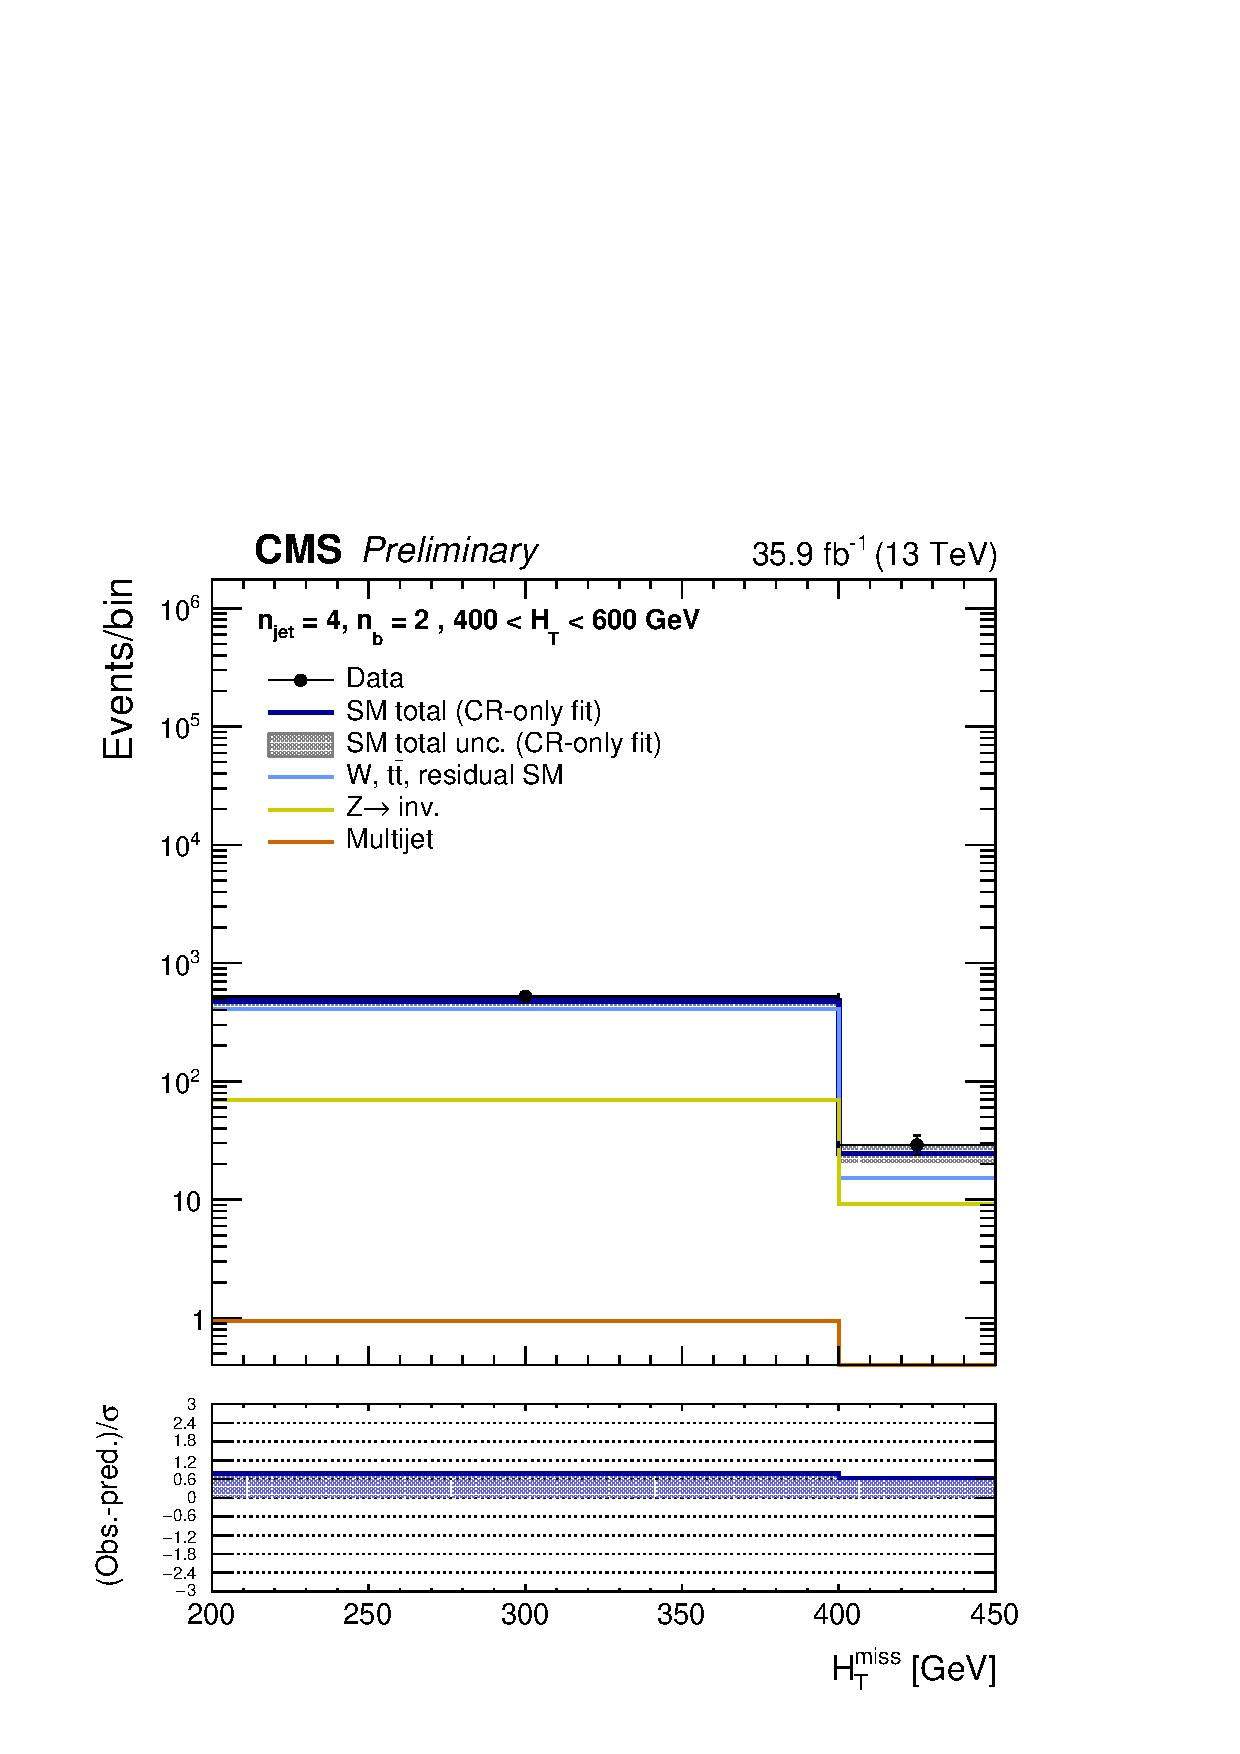
\includegraphics[width=0.49\textwidth]{figures/results/36invfb_preapproval//crfit/shapes//mhtShape_eq2b_eq4j_400_600_crfit.pdf}}
    \subfigure[$600 < \scalht < 900\GeV$]{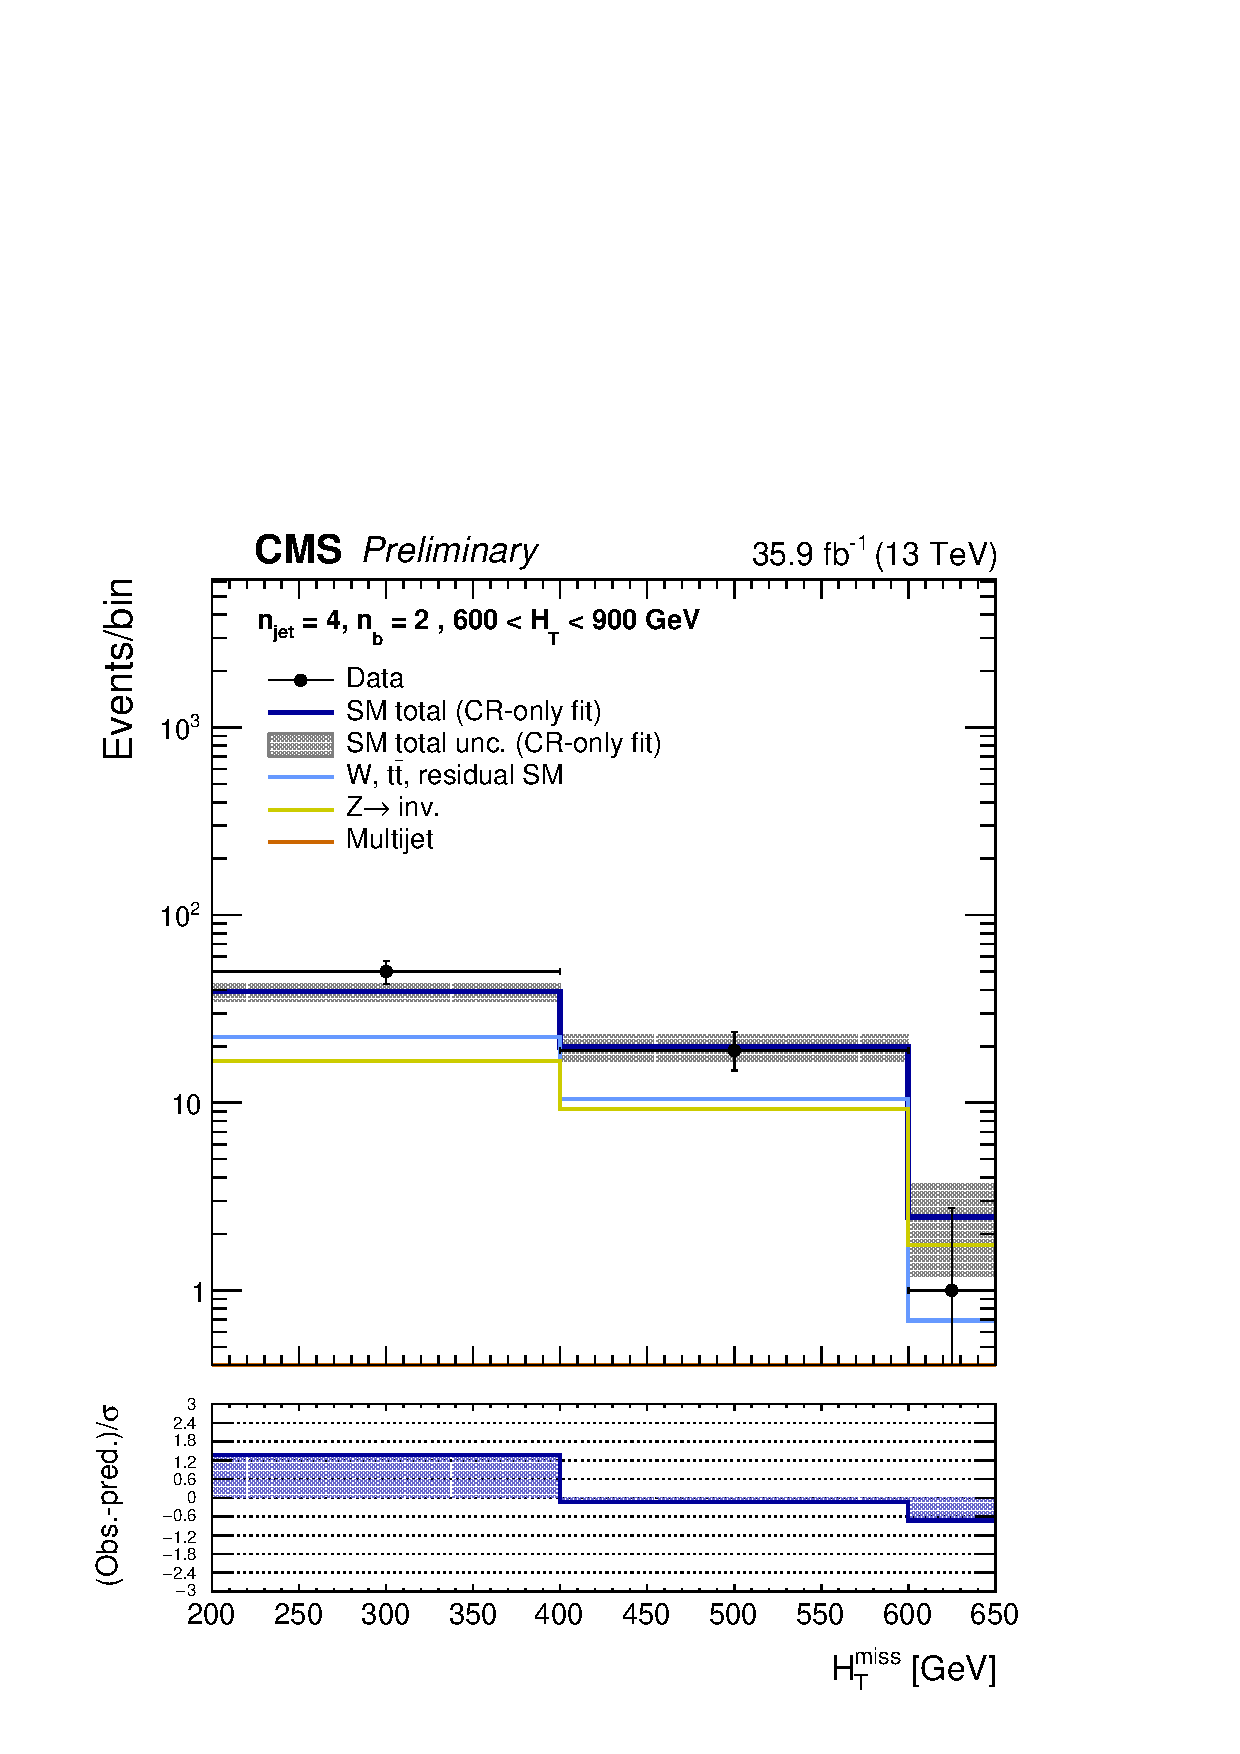
\includegraphics[width=0.49\textwidth]{figures/results/36invfb_preapproval//crfit/shapes//mhtShape_eq2b_eq4j_600_900_crfit.pdf}}\\
    \subfigure[$900 < \scalht < 1200\GeV$]{\includegraphics[width=0.49\textwidth]{figures/results/36invfb_preapproval//crfit/shapes//mhtShape_eq2b_eq4j_900_1200_crfit.pdf}}
    \subfigure[$\scalht > 1200\GeV$]{\includegraphics[width=0.49\textwidth]{figures/results/36invfb_preapproval//crfit/shapes//mhtShape_eq2b_eq4j_1200_Inf_crfit.pdf}}\\
    \caption{Event yields observed in data (solid circles) and CR-fit SM expectations with their associated uncertainties (green histogram with shaded band) as a function of \HTmiss based on a sample of events that satisfy $\njet = 4$ and $\nb = 2$, as well as the requirements on \scalht indicated by each sub-figure caption. }
    \label{fig:mhtdim_eq4j_eq2b}
  \end{center}
\end{figure}

\clearpage
\begin{figure}[h!]
  \begin{center}
    \subfigure[$400 < \scalht < 600\GeV$]{\includegraphics[width=0.49\textwidth]{figures/results/36invfb_preapproval//crfit/shapes//mhtShape_eq0b_eq5j_400_600_crfit.pdf}}
    \subfigure[$600 < \scalht < 900\GeV$]{\includegraphics[width=0.49\textwidth]{figures/results/36invfb_preapproval//crfit/shapes//mhtShape_eq0b_eq5j_600_900_crfit.pdf}}\\
    \subfigure[$900 < \scalht < 1200\GeV$]{\includegraphics[width=0.49\textwidth]{figures/results/36invfb_preapproval//crfit/shapes//mhtShape_eq0b_eq5j_900_1200_crfit.pdf}}
    \subfigure[$\scalht > 1200\GeV$]{\includegraphics[width=0.49\textwidth]{figures/results/36invfb_preapproval//crfit/shapes//mhtShape_eq0b_eq5j_1200_Inf_crfit.pdf}}\\
    \caption{Event yields observed in data (solid circles) and CR-fit SM expectations with their associated uncertainties (green histogram with shaded band) as a function of \HTmiss based on a sample of events that satisfy $\njet = 5$ and $\nb = 0$, as well as the requirements on \scalht indicated by each sub-figure caption. }
    \label{fig:mhtdim_eq5j_eq0b}
  \end{center}
\end{figure}

\clearpage
\begin{figure}[h!]
  \begin{center}
    \subfigure[$400 < \scalht < 600\GeV$]{\includegraphics[width=0.49\textwidth]{figures/results/36invfb_preapproval//crfit/shapes//mhtShape_eq1b_eq5j_400_600_crfit.pdf}}
    \subfigure[$600 < \scalht < 900\GeV$]{\includegraphics[width=0.49\textwidth]{figures/results/36invfb_preapproval//crfit/shapes//mhtShape_eq1b_eq5j_600_900_crfit.pdf}}\\
    \subfigure[$900 < \scalht < 1200\GeV$]{\includegraphics[width=0.49\textwidth]{figures/results/36invfb_preapproval//crfit/shapes//mhtShape_eq1b_eq5j_900_1200_crfit.pdf}}
    \subfigure[$\scalht > 1200\GeV$]{\includegraphics[width=0.49\textwidth]{figures/results/36invfb_preapproval//crfit/shapes//mhtShape_eq1b_eq5j_1200_Inf_crfit.pdf}}\\
    \caption{Event yields observed in data (solid circles) and CR-fit SM expectations with their associated uncertainties (green histogram with shaded band) as a function of \HTmiss based on a sample of events that satisfy $\njet = 5$ and $\nb = 1$, as well as the requirements on \scalht indicated by each sub-figure caption. }
    \label{fig:mhtdim_eq5j_eq1b}
  \end{center}
\end{figure}

\clearpage
\begin{figure}[h!]
  \begin{center}
    \subfigure[$400 < \scalht < 600\GeV$]{\includegraphics[width=0.49\textwidth]{figures/results/36invfb_preapproval//crfit/shapes//mhtShape_eq2b_eq5j_400_600_crfit.pdf}}
    \subfigure[$600 < \scalht < 900\GeV$]{\includegraphics[width=0.49\textwidth]{figures/results/36invfb_preapproval//crfit/shapes//mhtShape_eq2b_eq5j_600_900_crfit.pdf}}\\
    \subfigure[$900 < \scalht < 1200\GeV$]{\includegraphics[width=0.49\textwidth]{figures/results/36invfb_preapproval//crfit/shapes//mhtShape_eq2b_eq5j_900_1200_crfit.pdf}}
    \subfigure[$\scalht > 1200\GeV$]{\includegraphics[width=0.49\textwidth]{figures/results/36invfb_preapproval//crfit/shapes//mhtShape_eq2b_eq5j_1200_Inf_crfit.pdf}}\\
    \caption{Event yields observed in data (solid circles) and CR-fit SM expectations with their associated uncertainties (green histogram with shaded band) as a function of \HTmiss based on a sample of events that satisfy $\njet = 5$ and $\nb = 2$, as well as the requirements on \scalht indicated by each sub-figure caption. }
    \label{fig:mhtdim_eq5j_eq2b}
  \end{center}
\end{figure}

\clearpage
\begin{figure}[h!]
  \begin{center}
    \subfigure[$400 < \scalht < 600\GeV$]{\includegraphics[width=0.49\textwidth]{figures/results/36invfb_preapproval//crfit/shapes//mhtShape_eq3b_eq5j_400_600_crfit.pdf}}
    \subfigure[$600 < \scalht < 900\GeV$]{\includegraphics[width=0.49\textwidth]{figures/results/36invfb_preapproval//crfit/shapes//mhtShape_eq3b_eq5j_600_900_crfit.pdf}}\\
    \subfigure[$\scalht > 900\GeV$]{\includegraphics[width=0.49\textwidth]{figures/results/36invfb_preapproval//crfit/shapes//mhtShape_eq3b_eq5j_900_Inf_crfit.pdf}}
    \caption{Event yields observed in data (solid circles) and CR-fit SM expectations with their associated uncertainties (green histogram with shaded band) as a function of \HTmiss based on a sample of events that satisfy $\njet = 5$ and $\nb = 3$, as well as the requirements on \scalht indicated by each sub-figure caption. }
    \label{fig:mhtdim_eq5j_eq3b}
  \end{center}
\end{figure}

\clearpage
\begin{figure}[h!]
  \begin{center}
    \subfigure[$600 < \scalht < 900\GeV$]{\includegraphics[width=0.49\textwidth]{figures/results/36invfb_preapproval//crfit/shapes//mhtShape_eq0b_ge6j_600_900_crfit.pdf}}
    \subfigure[$900 < \scalht < 1200\GeV$]{\includegraphics[width=0.49\textwidth]{figures/results/36invfb_preapproval//crfit/shapes//mhtShape_eq0b_ge6j_900_1200_crfit.pdf}}\\
    \subfigure[$\scalht > 1200\GeV$]{\includegraphics[width=0.49\textwidth]{figures/results/36invfb_preapproval//crfit/shapes//mhtShape_eq0b_ge6j_1200_Inf_crfit.pdf}}
    \caption{Event yields observed in data (solid circles) and CR-fit SM expectations with their associated uncertainties (green histogram with shaded band) as a function of \HTmiss based on a sample of events that satisfy $\njet \geq 6$ and $\nb = 0$, as well as the requirements on \scalht indicated by each sub-figure caption. }
    \label{fig:mhtdim_ge6j_eq0b}
  \end{center}
\end{figure}

\clearpage
\begin{figure}[h!]
  \begin{center}
    \subfigure[$600 < \scalht < 900\GeV$]{\includegraphics[width=0.49\textwidth]{figures/results/36invfb_preapproval//crfit/shapes//mhtShape_eq1b_ge6j_600_900_crfit.pdf}}
    \subfigure[$900 < \scalht < 1200\GeV$]{\includegraphics[width=0.49\textwidth]{figures/results/36invfb_preapproval//crfit/shapes//mhtShape_eq1b_ge6j_900_1200_crfit.pdf}}\\
    \subfigure[$\scalht > 1200\GeV$]{\includegraphics[width=0.49\textwidth]{figures/results/36invfb_preapproval//crfit/shapes//mhtShape_eq1b_ge6j_1200_Inf_crfit.pdf}}
    \caption{Event yields observed in data (solid circles) and CR-fit SM expectations with their associated uncertainties (green histogram with shaded band) as a function of \HTmiss based on a sample of events that satisfy $\njet \geq 6$ and $\nb = 1$, as well as the requirements on \scalht indicated by each sub-figure caption. }
    \label{fig:mhtdim_ge6j_eq1b}
  \end{center}
\end{figure}

\clearpage
\begin{figure}[h!]
  \begin{center}
    \subfigure[$600 < \scalht < 900\GeV$]{\includegraphics[width=0.49\textwidth]{figures/results/36invfb_preapproval//crfit/shapes//mhtShape_eq2b_ge6j_600_900_crfit.pdf}}
    \subfigure[$900 < \scalht < 1200\GeV$]{\includegraphics[width=0.49\textwidth]{figures/results/36invfb_preapproval//crfit/shapes//mhtShape_eq2b_ge6j_900_1200_crfit.pdf}}\\
    \subfigure[$\scalht > 1200\GeV$]{\includegraphics[width=0.49\textwidth]{figures/results/36invfb_preapproval//crfit/shapes//mhtShape_eq2b_ge6j_1200_Inf_crfit.pdf}}
    \caption{Event yields observed in data (solid circles) and CR-fit SM expectations with their associated uncertainties (green histogram with shaded band) as a function of \HTmiss based on a sample of events that satisfy $\njet \geq 6$ and $\nb = 2$, as well as the requirements on \scalht indicated by each sub-figure caption. }
    \label{fig:mhtdim_ge6j_eq2b}
  \end{center}
\end{figure}

\clearpage
\begin{figure}[h!]
  \begin{center}
    \subfigure[$600 < \scalht < 900\GeV$]{\includegraphics[width=0.49\textwidth]{figures/results/36invfb_preapproval//crfit/shapes//mhtShape_eq3b_ge6j_600_900_crfit.pdf}}
    \subfigure[$900 < \scalht < 1200\GeV$]{\includegraphics[width=0.49\textwidth]{figures/results/36invfb_preapproval//crfit/shapes//mhtShape_eq3b_ge6j_900_1200_crfit.pdf}}\\
    \subfigure[$\scalht > 1200\GeV$]{\includegraphics[width=0.49\textwidth]{figures/results/36invfb_preapproval//crfit/shapes//mhtShape_eq3b_ge6j_1200_Inf_crfit.pdf}}
    \caption{Event yields observed in data (solid circles) and CR-fit SM expectations with their associated uncertainties (green histogram with shaded band) as a function of \HTmiss based on a sample of events that satisfy $\njet \geq 6$ and $\nb = 3$, as well as the requirements on \scalht indicated by each sub-figure caption. }
    \label{fig:mhtdim_ge6j_eq3b}
  \end{center}
\end{figure}
